% ============================================================
% APPENDIX
% ============================================================

\clearpage
\appendix

\begin{center}
    {\large\bfseries APPENDIX}
\end{center}

% Start appendix-only TOC
\startcontents[appendix]
\printcontents[appendix]{}{1}{
    \setcounter{tocdepth}{2}
}

\pagenumbering{arabic}
\renewcommand{\thepage}{\Alph{section}-\arabic{page}}
\renewcommand{\thesection}{\Alph{section}}
\renewcommand{\thefigure}{\Alph{figure}}
\renewcommand{\thetable}{\Alph{table}}

\setcounter{section}{0}
\setcounter{figure}{0}
\setcounter{table}{0}
\setcounter{page}{1}

\newpage
\section{Additional results}
\label{sec:additional_results_suppl}
\subsection{Point Cloud and Pose Degradation with Increasing Fraction of Rotated Images}
\label{sec:fraction_degradation}
To complement the results presented in \Cref{tab:rotation_degradation_main}, we report the corresponding degradation results for the remaining datasets (Tanks \& Temples, Mip-NeRF 360, DTU and RotMV) in \Cref{tab:supplementary_rotation_degradation}. These additional results consistently shows how point cloud reconstruction and pose estimation performance change as the fraction of rotated input images increases, extending the analysis across all evaluated datasets.

\definecolor{datasetbg}{gray}{0.94}

% Helper command to shift std dev right using left-alignment and offset spacing
\begin{table}[h]
    \centering
    \caption{Point-map and camera-pose estimation performance under increasing fractions of rotated input views. Feed Forward models suffers consistent degradation as fraction of rotated frames increases}
    \label{tab:supplementary_rotation_degradation}
    \small
    \setlength{\tabcolsep}{4.5pt}

\begin{tabular}{@{}ll ccccc ccccc@{}}
        \toprule
        & & \multicolumn{5}{c}{\textbf{Point-map Estimation (N.C.)}}
        & \multicolumn{5}{c}{\textbf{Camera Pose Estimation (AUC$_{30}$)}} \\
        \cmidrule(lr){3-7} \cmidrule(lr){8-12}
        & \textbf{Rot.}
        & VGGT & VGGT-$\Omega$ & $\pi^3$ & MapA. & DA3
        & VGGT & VGGT-$\Omega$ & $\pi^3$ & MapA. & DA3 \\
        \midrule

        % Tanks\&Temples (White / Default background)
        & 0\%   & \valstd{0.665}{0.076} & \valstd{0.724}{0.067} & \valstd{0.707}{0.118} & \valstd{0.628}{0.152} & \valstd{0.707}{0.064}
                & \valstd{76.4}{35.5} & \valstd{91.1}{16.1} & \valstd{79.6}{28.4} & \valstd{78.3}{22.7} & \valstd{94.2}{8.2} \\
        & 25\%  & \valstd{0.641}{0.030} & \valstd{0.725}{0.017} & \valstd{0.684}{0.032} & \valstd{0.613}{0.029} & \valstd{0.664}{0.039}
                & \valstd{66.6}{8.6} & \valstd{87.9}{3.2} & \valstd{67.7}{5.5} & \valstd{56.5}{8.9} & \valstd{62.6}{17.0} \\
        & 50\%  & \valstd{0.641}{0.050} & \valstd{0.712}{0.018} & \valstd{0.656}{0.038} & \valstd{0.598}{0.038} & \valstd{0.650}{0.046}
                & \valstd{57.2}{11.7} & \valstd{83.0}{4.2} & \valstd{56.1}{7.9} & \valstd{37.6}{12.5} & \valstd{47.8}{15.8} \\
        & 75\%  & \valstd{0.625}{0.046} & \valstd{0.703}{0.017} & \valstd{0.646}{0.031} & \valstd{0.595}{0.052} & \valstd{0.626}{0.036}
                & \valstd{49.5}{11.7} & \valstd{79.0}{7.1} & \valstd{48.5}{8.6} & \valstd{27.2}{9.8} & \valstd{34.5}{15.4} \\
        \multirow{-7}{*}{\rotatebox[origin=c]{90}{\textbf{Tanks\&Temples}}}
        & 100\% & \valstd{0.604}{0.043} & \valstd{0.685}{0.023} & \valstd{0.618}{0.040} & \valstd{0.572}{0.044} & \valstd{0.618}{0.042}
                & \valstd{42.7}{9.6} & \valstd{74.4}{7.2} & \valstd{40.7}{6.9} & \valstd{18.8}{6.1} & \valstd{31.6}{10.0} \\
        \addlinespace[3pt]

        % MipNeRF (Shaded background)
        % \rowcolor{datasetbg}
        % & 0\%   & \valstd{0.748}{0.101} & \valstd{0.742}{0.078} & \valstd{0.734}{0.088} & \valstd{0.725}{0.119} & \valstd{0.717}{0.055}
        %         & \valstd{96.1}{2.8} & \valstd{97.8}{1.4} & \valstd{96.7}{2.2} & \valstd{90.7}{7.0} & \valstd{98.5}{0.8} \\
        \rowcolor{datasetbg}
        & 25\%  & \valstd{0.712}{0.025} & \valstd{0.711}{0.016} & \valstd{0.704}{0.013} & \valstd{0.660}{0.070} & \valstd{0.671}{0.028}
                & \valstd{90.1}{8.3} & \valstd{95.0}{1.7} & \valstd{90.8}{2.5} & \valstd{72.4}{10.1} & \valstd{82.4}{11.6} \\
        \rowcolor{datasetbg}
        & 50\%  & \valstd{0.685}{0.020} & \valstd{0.690}{0.013} & \valstd{0.676}{0.015} & \valstd{0.638}{0.059} & \valstd{0.656}{0.024}
                & \valstd{87.2}{5.9} & \valstd{92.6}{2.8} & \valstd{85.3}{3.6} & \valstd{59.2}{12.4} & \valstd{72.4}{11.2} \\
        \rowcolor{datasetbg}
        & 75\%  & \valstd{0.664}{0.018} & \valstd{0.673}{0.013} & \valstd{0.649}{0.013} & \valstd{0.614}{0.050} & \valstd{0.633}{0.022}
                & \valstd{83.5}{7.0} & \valstd{89.9}{2.5} & \valstd{80.0}{7.5} & \valstd{49.4}{10.5} & \valstd{65.4}{11.0} \\
        \rowcolor{datasetbg}
        \multirow{-7}{*}[0pt]{\rotatebox[origin=c]{90}{\footnotesize\textbf{Mip-NeRF 360}$^{*}$}}
        & 100\% & \valstd{0.643}{0.011} & \valstd{0.654}{0.014} & \valstd{0.623}{0.011} & \valstd{0.591}{0.051} & \valstd{0.615}{0.020}
                & \valstd{74.9}{7.8} & \valstd{87.4}{2.4} & \valstd{73.8}{4.7} & \valstd{42.7}{9.9} & \valstd{63.1}{9.7} \\
        \addlinespace[3pt]

        % DTU (White / Default background)
        & 0\%   & \valstd{0.611}{0.048} & \valstd{0.634}{0.020} & \valstd{0.621}{0.032} & \valstd{0.577}{0.062} & \valstd{0.585}{0.054}
                & \valstd{77.5}{18.7} & \valstd{93.2}{6.9} & \valstd{85.6}{11.6} & \valstd{33.0}{23.0} & \valstd{59.8}{25.5} \\
        & 25\%  & \valstd{0.630}{0.027} & \valstd{0.629}{0.025} & \valstd{0.625}{0.025} & \valstd{0.625}{0.047} & \valstd{0.619}{0.035}
                & \valstd{88.6}{14.1} & \valstd{95.1}{2.2} & \valstd{90.1}{7.6} & \valstd{36.5}{15.0} & \valstd{83.1}{12.9} \\
        & 50\%  & \valstd{0.625}{0.030} & \valstd{0.632}{0.012} & \valstd{0.632}{0.015} & \valstd{0.598}{0.039} & \valstd{0.590}{0.043}
                & \valstd{83.9}{16.8} & \valstd{94.6}{3.2} & \valstd{89.9}{5.5} & \valstd{41.8}{18.7} & \valstd{68.1}{22.3} \\
        & 75\%  & \valstd{0.631}{0.023} & \valstd{0.632}{0.017} & \valstd{0.634}{0.011} & \valstd{0.620}{0.034} & \valstd{0.621}{0.038}
                & \valstd{91.8}{9.1} & \valstd{94.5}{2.6} & \valstd{90.8}{5.2} & \valstd{57.7}{17.2} & \valstd{74.5}{18.8} \\
        \multirow{-7}{*}{\rotatebox[origin=c]{90}{\textbf{DTU}}}
        & 100\% & \valstd{0.619}{0.017} & \valstd{0.621}{0.011} & \valstd{0.615}{0.011} & \valstd{0.568}{0.029} & \valstd{0.587}{0.028}
                & \valstd{79.6}{21.9} & \valstd{93.7}{3.4} & \valstd{84.7}{10.4} & \valstd{39.6}{17.7} & \valstd{63.4}{32.8} \\
        \addlinespace[3pt]

        % RotMV (Shaded background)
        % \rowcolor{datasetbg}
        % & 0\%   & \valstd{1.000}{0.000} & \valstd{1.000}{0.000} & \valstd{1.000}{0.000} & \valstd{0.914}{0.059} & \valstd{0.966}{0.064}
        %         & \valstd{100.0}{0.0} & \valstd{98.8}{1.0} & \valstd{98.4}{1.0} & \valstd{96.4}{1.6} & \valstd{98.8}{0.9} \\
        \rowcolor{datasetbg}
        & 25\%  & \valstd{0.735}{0.048} & \valstd{0.755}{0.028} & \valstd{0.738}{0.054} & \valstd{0.749}{0.090} & \valstd{0.749}{0.038}
                & \valstd{88.5}{7.2} & \valstd{91.7}{3.6} & \valstd{86.1}{6.2} & \valstd{68.9}{16.4} & \valstd{80.3}{10.0} \\
        \rowcolor{datasetbg}
        & 50\%  & \valstd{0.673}{0.050} & \valstd{0.707}{0.028} & \valstd{0.696}{0.047} & \valstd{0.676}{0.083} & \valstd{0.689}{0.061}
                & \valstd{74.4}{13.2} & \valstd{85.1}{4.4} & \valstd{77.1}{8.2} & \valstd{46.3}{18.6} & \valstd{58.7}{21.2} \\
        \rowcolor{datasetbg}
        & 75\%  & \valstd{0.644}{0.056} & \valstd{0.687}{0.014} & \valstd{0.668}{0.045} & \valstd{0.639}{0.079} & \valstd{0.651}{0.063}
                & \valstd{66.4}{16.1} & \valstd{80.5}{3.9} & \valstd{69.0}{11.4} & \valstd{36.4}{14.5} & \valstd{48.4}{19.8} \\
        \rowcolor{datasetbg}
        \multirow{-6}{*}{\rotatebox[origin=c]{90}{\textbf{RotMV$^{*}$}}}
        & 100\% & \valstd{0.626}{0.049} & \valstd{0.670}{0.015} & \valstd{0.654}{0.039} & \valstd{0.603}{0.052} & \valstd{0.659}{0.045}
                & \valstd{56.6}{17.6} & \valstd{75.5}{5.0} & \valstd{63.9}{10.7} & \valstd{21.4}{11.8} & \valstd{52.3}{14.4} \\
        \bottomrule

\end{tabular}
\par\vspace{3pt}
{\footnotesize\raggedright
$^{*}$Mip-NeRF 360 and RotMV provide no ground-truth point clouds. For these datasets, both point-map and pose metrics are computed relative to each model's prediction on all upright (0\%) input (see ~\Cref{sec:eval_criteria}) beacuse of its SOTA performance on upright images. We measure degradation from all upright prediction. The 0\% setting would compare a prediction with itself and is hence omitted.\par}
\end{table}

\subsection{Performance on Additional Datasets}
\label{sec:remaining_results_suppl}

We include results on the remaining datasets for comparison with ROVER and baselines, specifically MipNerf-360\citep{barron2022mipnerf360}, Tanks and Temples \cite{Knapitsch2017tanksandtemples}, DTU \cite{jensen2014largeDTU} and ETH3D ~\citep{Schops_2019_CVPRETH3D1, schoeps2017cvprETH3D2}. ~\Cref{tab:pointmap_rover_format_suppl} and ~\Cref{tab:pointmap_eth3d_dtu_suppl} presents point-map estimation results, whereas ~\Cref{tab:pose_rover_format_suppl} and ~\Cref{tab:pose_eth3d_dtu_suppl} present the corresponding camera pose estimation results. We observe ROVER helps improve the reconstruction by consistently re-canonicalizing the input images before using the feed forward reconstruction model. In ~\Cref{tab:pointmap_eth3d_dtu_suppl} and ~\Cref{tab:pose_eth3d_dtu_suppl}, we observe ETH3D gains are consistent across all models and metrics with VGGT-$\Omega$ and $\pi^3$ showing consistent gains ($95.07$ to $95.26$ and $81.89$ to $83.80$) in AUC$_{30}$, while VGGT shows increase in TAcc$_{30}$ ($87.57$ to $89.80$). Overall, our approach consistently recovers camera pose estimation quality under arbitrary in-plane rotations, with gains scaling with the severity of baseline degradation.
\begin{table}[H]
\centering
\caption{Point map estimation on Tanks\&Temples and Mip-NeRF 360 datasets. ROVER consistently improves performance of feed forward models by canocalizing input images.}
\label{tab:pointmap_rover_format_suppl}
\small
\renewcommand{\arraystretch}{1.5}
\setlength{\tabcolsep}{4pt}
\providecommand{\dd}[2]{\makecell{#1 \\ {\tiny $\pm$ #2}}}

\resizebox{\linewidth}{!}{
\begin{tabular}{l *{3}{cc} *{3}{cc}}
\toprule
 & \multicolumn{6}{c}{\textbf{Tanks\&Temples}} & \multicolumn{6}{c}{\textbf{Mip-NeRF 360}} \\
\cmidrule(lr){2-7} \cmidrule(lr){8-13}
 & \multicolumn{2}{c}{Acc. $\downarrow$} & \multicolumn{2}{c}{Comp. $\downarrow$} & \multicolumn{2}{c}{N.C. $\uparrow$} & \multicolumn{2}{c}{Acc. $\downarrow$} & \multicolumn{2}{c}{Comp. $\downarrow$} & \multicolumn{2}{c}{N.C. $\uparrow$} \\
\cmidrule(lr){2-3} \cmidrule(lr){4-5} \cmidrule(lr){6-7} \cmidrule(lr){8-9} \cmidrule(lr){10-11} \cmidrule(lr){12-13}
\textbf{Method} & Base & Ours & Base & Ours & Base & Ours & Base & Ours & Base & Ours & Base & Ours \\
\midrule

VGGT & \dd{0.322}{0.098} & \dd{\textbf{0.247}}{0.045} & \dd{0.594}{0.336} & \dd{\textbf{0.539}}{0.214} & \dd{0.629}{0.055} & \dd{\textbf{0.648}}{0.046} & \dd{0.021}{0.006} & \dd{\textbf{0.014}}{0.003} & \dd{0.040}{0.023} & \dd{\textbf{0.019}}{0.004} & \dd{0.678}{0.034} & \dd{\textbf{0.726}}{0.025} \\
\addlinespace[3pt]

VGGT-$\Omega$ & \dd{0.190}{0.048} & \dd{\textbf{0.157}}{0.025} & \dd{0.143}{0.058} & \dd{\textbf{0.126}}{0.032} & \dd{0.707}{0.028} & \dd{\textbf{0.719}}{0.021} & \dd{0.017}{0.004} & \dd{\textbf{0.014}}{0.002} & \dd{0.017}{0.005} & \dd{\textbf{0.013}}{0.002} & \dd{0.684}{0.028} & \dd{\textbf{0.714}}{0.020} \\
\addlinespace[3pt]

$\pi^3$ & \dd{0.291}{0.100} & \dd{\textbf{0.199}}{0.041} & \dd{0.415}{0.173} & \dd{\textbf{0.347}}{0.081} & \dd{0.652}{0.049} & \dd{\textbf{0.689}}{0.032} & \dd{0.042}{0.015} & \dd{\textbf{0.026}}{0.005} & \dd{0.062}{0.035} & \dd{\textbf{0.034}}{0.009} & \dd{0.665}{0.037} & \dd{\textbf{0.711}}{0.023} \\
\addlinespace[3pt]

MapA. & \dd{0.340}{0.107} & \dd{\textbf{0.297}}{0.051} & \dd{0.808}{0.398} & \dd{\textbf{0.776}}{0.253} & \dd{0.595}{0.049} & \dd{\textbf{0.622}}{0.033} & \dd{0.351}{0.144} & \dd{\textbf{0.260}}{0.079} & \dd{0.568}{0.288} & \dd{\textbf{0.407}}{0.196} & \dd{0.628}{0.068} & \dd{\textbf{0.665}}{0.070} \\
\addlinespace[3pt]

DA3 & \dd{0.407}{0.155} & \dd{\textbf{0.275}}{0.063} & \dd{0.534}{0.335} & \dd{\textbf{0.335}}{0.117} & \dd{0.641}{0.049} & \dd{\textbf{0.674}}{0.033} & \dd{0.319}{0.169} & \dd{\textbf{0.162}}{0.069} & \dd{0.396}{0.381} & \dd{\textbf{0.156}}{0.067} & \dd{0.646}{0.035} & \dd{\textbf{0.683}}{0.026} \\
\addlinespace[3pt]

\bottomrule
\end{tabular}

% 2 Outliers Excluded: scan13 and scan29 [has some variations in pitch/yaw].
% scan11 Excluded: angle renders were poor and were excluded.
}
\end{table}

\begin{table}[h]
\centering
\caption{Camera pose estimation on Tanks\&Temples and Mip-NeRF 360 datasets. We observe ROVER helps recover performance of feed forward models}
\label{tab:pose_rover_format_suppl}
\small
\renewcommand{\arraystretch}{1.2}
\setlength{\tabcolsep}{2pt}
\providecommand{\dd}[2]{\makecell{#1 \\ {\tiny $\pm$ #2}}}

\resizebox{\linewidth}{!}{
\begin{tabular}{l *{3}{cc} *{3}{cc}}
\toprule
 & \multicolumn{6}{c}{\textbf{Tanks\&Temples}} & \multicolumn{6}{c}{\textbf{Mip-NeRF 360}} \\
\cmidrule(lr){2-7} \cmidrule(lr){8-13}
 & \multicolumn{2}{c}{RAcc$_{30}$ $\uparrow$} & \multicolumn{2}{c}{TAcc$_{30}$ $\uparrow$} & \multicolumn{2}{c}{AUC$_{30}$ $\uparrow$} & \multicolumn{2}{c}{RAcc$_{30}$ $\uparrow$} & \multicolumn{2}{c}{TAcc$_{30}$ $\uparrow$} & \multicolumn{2}{c}{AUC$_{30}$ $\uparrow$} \\
\cmidrule(lr){2-3} \cmidrule(lr){4-5} \cmidrule(lr){6-7} \cmidrule(lr){8-9} \cmidrule(lr){10-11} \cmidrule(lr){12-13}
\textbf{Method} & Base & Ours & Base & Ours & Base & Ours & Base & Ours & Base & Ours & Base & Ours \\
\midrule

VGGT & \dd{70.419}{16.405} & \dd{\textbf{86.028}}{6.329} & \dd{73.793}{11.929} & \dd{\textbf{84.134}}{4.598} & \dd{54.563}{14.883} & \dd{\textbf{72.567}}{4.997} & \dd{95.961}{5.195} & \dd{\textbf{100.000}}{0.000} & \dd{96.069}{4.732} & \dd{\textbf{99.872}}{0.278} & \dd{84.226}{9.689} & \dd{\textbf{93.703}}{2.519} \\
\addlinespace[3pt]

VGGT-$\Omega$ & \dd{98.780}{3.576} & \dd{\textbf{99.610}}{1.424} & \dd{93.049}{4.217} & \dd{\textbf{93.870}}{2.607} & \dd{81.307}{7.807} & \dd{\textbf{87.009}}{4.083} & \dd{99.956}{0.279} & \dd{\textbf{100.000}}{0.000} & \dd{99.541}{0.772} & \dd{\textbf{99.948}}{0.145} & \dd{91.373}{3.887} & \dd{\textbf{96.458}}{1.191} \\
\addlinespace[3pt]

$\pi^3$ & \dd{70.350}{11.942} & \dd{\textbf{87.248}}{2.603} & \dd{72.386}{9.104} & \dd{\textbf{83.846}}{1.889} & \dd{53.893}{13.126} & \dd{\textbf{74.584}}{4.079} & \dd{96.141}{5.166} & \dd{\textbf{100.000}}{0.000} & \dd{96.828}{4.049} & \dd{\textbf{99.768}}{0.338} & \dd{82.922}{8.558} & \dd{\textbf{92.765}}{2.403} \\
\addlinespace[3pt]

MapA. & \dd{59.961}{18.558} & \dd{\textbf{83.504}}{7.109} & \dd{63.738}{13.405} & \dd{\textbf{80.606}}{6.166} & \dd{36.130}{18.636} & \dd{\textbf{62.529}}{10.936} & \dd{87.015}{12.013} & \dd{\textbf{95.967}}{5.741} & \dd{86.318}{10.531} & \dd{\textbf{95.656}}{5.312} & \dd{56.776}{16.878} & \dd{\textbf{75.265}}{9.465} \\
\addlinespace[3pt]

DA3 & \dd{63.829}{19.325} & \dd{\textbf{87.285}}{8.889} & \dd{68.695}{15.722} & \dd{\textbf{86.463}}{8.416} & \dd{45.356}{21.409} & \dd{\textbf{75.814}}{11.952} & \dd{86.272}{11.855} & \dd{\textbf{98.685}}{2.499} & \dd{90.395}{9.753} & \dd{\textbf{99.036}}{1.549} & \dd{71.490}{15.075} & \dd{\textbf{91.869}}{6.288} \\
\addlinespace[3pt]

\bottomrule
\end{tabular}
}
\end{table}
\begin{table}[tbp]
\centering
\caption{Point map estimation on ETH3D and DTU datasets. ROVER consistently improves performance of feed forward models by canocalizing input images.}
\label{tab:pointmap_eth3d_dtu_suppl}
\small
\renewcommand{\arraystretch}{1.2}
\setlength{\tabcolsep}{4pt}
\providecommand{\dd}[2]{\makecell{#1 \\ {\tiny $\pm$ #2}}}

\resizebox{\linewidth}{!}{
\begin{tabular}{l *{3}{cc} *{3}{cc}}
\toprule
 & \multicolumn{6}{c}{\textbf{ETH3D}} & \multicolumn{6}{c}{\textbf{DTU}} \\
\cmidrule(lr){2-7} \cmidrule(lr){8-13}
 & \multicolumn{2}{c}{Acc. $\downarrow$} & \multicolumn{2}{c}{Comp. $\downarrow$} & \multicolumn{2}{c}{N.C. $\uparrow$} & \multicolumn{2}{c}{Acc. $\downarrow$} & \multicolumn{2}{c}{Comp. $\downarrow$} & \multicolumn{2}{c}{N.C. $\uparrow$} \\
\cmidrule(lr){2-3} \cmidrule(lr){4-5} \cmidrule(lr){6-7} \cmidrule(lr){8-9} \cmidrule(lr){10-11} \cmidrule(lr){12-13}
\textbf{Method} & Base & Ours & Base & Ours & Base & Ours & Base & Ours & Base & Ours & Base & Ours \\
\midrule

VGGT & \dd{0.20}{0.07} & \dd{\textbf{0.18}}{0.06} & \dd{0.11}{0.04} & \dd{\textbf{0.08}}{0.02} & \dd{0.77}{0.04} & \dd{\textbf{0.79}}{0.03} & \dd{4.306}{5.377} & \dd{\textbf{4.222}}{5.690} & \dd{\textbf{5.881}}{9.698} & \dd{6.488}{12.658} & \dd{\textbf{0.626}}{0.034} & \dd{0.624}{0.032} \\
\addlinespace[3pt]

VGGT-$\Omega$ & \dd{0.07}{0.03} & \dd{\textbf{0.06}}{0.02} & \dd{\textbf{0.05}}{0.02} & \dd{\textbf{0.05}}{0.02} & \dd{\textbf{0.85}}{0.03} & \dd{\textbf{0.85}}{0.03} & \dd{4.306}{5.377} & \dd{\textbf{2.144}}{1.976} & \dd{5.881}{9.698} & \dd{\textbf{2.273}}{2.620} & \dd{0.626}{0.034} & \dd{\textbf{0.630}}{0.019} \\
\addlinespace[3pt]

$\pi^3$ & \dd{0.09}{0.03} & \dd{\textbf{0.08}}{0.02} & \dd{0.07}{0.02} & \dd{\textbf{0.06}}{0.02} & \dd{0.84}{0.02} & \dd{\textbf{0.85}}{0.02} & \dd{2.441}{2.464} & \dd{\textbf{2.240}}{2.267} & \dd{2.784}{4.381} & \dd{\textbf{2.493}}{3.418} & \dd{\textbf{0.629}}{0.022} & \dd{\textbf{0.629}}{0.020} \\
\addlinespace[3pt]

MapA. & \dd{0.16}{0.03} & \dd{\textbf{0.15}}{0.03} & \dd{0.39}{0.36} & \dd{\textbf{0.36}}{0.29} & \dd{0.75}{0.03} & \dd{\textbf{0.76}}{0.02} & \dd{12.201}{5.185} & \dd{\textbf{12.146}}{5.140} & \dd{19.941}{13.894} & \dd{\textbf{18.567}}{12.641} & \dd{\textbf{0.602}}{0.047} & \dd{\textbf{0.602}}{0.043} \\
\addlinespace[3pt]

DA3 & \dd{\textbf{0.11}}{0.02} & \dd{\textbf{0.11}}{0.00} & \dd{0.12}{0.01} & \dd{\textbf{0.10}}{0.01} & \dd{\textbf{0.82}}{0.01} & \dd{\textbf{0.82}}{0.01} & \dd{7.979}{5.250} & \dd{\textbf{7.441}}{6.222} & \dd{13.492}{15.661} & \dd{\textbf{10.556}}{14.709} & \dd{0.608}{0.046} & \dd{\textbf{0.614}}{0.041} \\
\addlinespace[3pt]

\bottomrule
\end{tabular}

% 2 Outliers Excluded: scan13 and scan29 [has some variations in pitch/yaw].
% scan11 Excluded: angle renders were poor and were excluded.
}
\end{table}
\begin{table}[h]
\centering
\caption{Camera pose estimation on ETH3D and DTU datasets. We observe ROVER helps recover performance of feed forward models}
\label{tab:pose_eth3d_dtu_suppl}
\small
\renewcommand{\arraystretch}{1.2}
\setlength{\tabcolsep}{4pt}
\providecommand{\dd}[2]{\makecell{#1 \\ {\tiny $\pm$ #2}}}

\resizebox{\linewidth}{!}{
\begin{tabular}{l *{3}{cc} *{3}{cc}}
\toprule
 & \multicolumn{6}{c}{\textbf{ETH3D}} & \multicolumn{6}{c}{\textbf{DTU}} \\
\cmidrule(lr){2-7} \cmidrule(lr){8-13}
 & \multicolumn{2}{c}{RAcc$_{30}$ $\uparrow$} & \multicolumn{2}{c}{TAcc$_{30}$ $\uparrow$} & \multicolumn{2}{c}{AUC$_{30}$ $\uparrow$} & \multicolumn{2}{c}{RAcc$_{30}$ $\uparrow$} & \multicolumn{2}{c}{TAcc$_{30}$ $\uparrow$} & \multicolumn{2}{c}{AUC$_{30}$ $\uparrow$} \\
\cmidrule(lr){2-3} \cmidrule(lr){4-5} \cmidrule(lr){6-7} \cmidrule(lr){8-9} \cmidrule(lr){10-11} \cmidrule(lr){12-13}
\textbf{Method} & Base & Ours & Base & Ours & Base & Ours & Base & Ours & Base & Ours & Base & Ours \\
\midrule

VGGT & \dd{93.03}{13.02} & \dd{\textbf{94.02}}{13.86} & \dd{87.57}{14.92} & \dd{\textbf{89.80}}{14.96} & \dd{70.54}{22.51} & \dd{\textbf{72.81}}{22.81} & \dd{94.376}{13.945} & \dd{\textbf{97.275}}{9.516} & \dd{94.969}{11.294} & \dd{\textbf{97.631}}{7.825} & \dd{86.101}{18.090} & \dd{\textbf{91.598}}{12.317} \\
\addlinespace[3pt]

VGGT-$\Omega$ & \dd{99.98}{0.08} & \dd{\textbf{100.00}}{0.00} & \dd{99.79}{0.26} & \dd{\textbf{99.82}}{0.52} & \dd{95.07}{2.80} & \dd{\textbf{95.26}}{2.58} & \dd{94.376}{13.945} & \dd{\textbf{99.790}}{3.404} & \dd{94.969}{11.294} & \dd{\textbf{99.791}}{3.197} & \dd{86.101}{18.090} & \dd{\textbf{95.274}}{5.058} \\
\addlinespace[3pt]

$\pi^3$ & \dd{96.35}{5.99} & \dd{\textbf{96.75}}{7.70} & \dd{95.51}{5.83} & \dd{\textbf{96.23}}{6.34} & \dd{81.89}{12.70} & \dd{\textbf{83.80}}{12.70} & \dd{98.968}{5.622} & \dd{\textbf{99.463}}{3.242} & \dd{98.770}{5.083} & \dd{\textbf{99.404}}{2.926} & \dd{88.982}{9.397} & \dd{\textbf{91.402}}{6.224} \\
\addlinespace[3pt]

MapA. & \dd{89.93}{12.44} & \dd{\textbf{90.24}}{13.34} & \dd{81.10}{16.54} & \dd{\textbf{81.87}}{16.98} & \dd{57.25}{16.32} & \dd{\textbf{57.72}}{17.40} & \dd{84.536}{21.317} & \dd{\textbf{90.301}}{15.862} & \dd{76.994}{21.675} & \dd{\textbf{81.775}}{17.298} & \dd{46.868}{22.298} & \dd{\textbf{50.393}}{19.157} \\
\addlinespace[3pt]

DA3 & \dd{87.74}{12.92} & \dd{\textbf{88.38}}{16.78} & \dd{88.16}{15.58} & \dd{\textbf{88.90}}{18.02} & \dd{79.62}{17.07} & \dd{\textbf{79.73}}{20.59} & \dd{89.745}{17.853} & \dd{\textbf{92.648}}{15.361} & \dd{89.612}{16.658} & \dd{\textbf{92.150}}{14.054} & \dd{73.804}{23.601} & \dd{\textbf{77.048}}{22.030} \\
\addlinespace[3pt]

\bottomrule
\end{tabular}
}
\end{table}
% ------------------------------------------------------------
\subsection{Results on RotMV}
\label{sec:rover_on_rotmv}
RotMV provides a complementary evaluation to our controlled rotation synthesis benchmarks: rather than rendering rotations in camera space, it consists of real-world multi-view sequences captured at arbitrary orientations, without black-padding or rendering artifacts. This makes it a more challenging and authentic test of whether our method generalizes beyond controlled synthetic perturbations.

~\Cref{tab:pointmap_combined} and ~\Cref{tab:pose_combined_restructured} in the main paper report point-map and camera pose estimation results respectively on RotMV. ROVER consistently improves over all base models across both tasks, confirming that the DINOv2 variance signal transfers reliably to real-world rotated captures. Notably, the gains on RotMV are consistent with those observed on synthetic benchmarks, suggesting that its orientation estimates are robust to the additional photometric variation and capture noise present in real-world sequences.
These results validate that our approach addresses UprightBias effectively without any retraining. The RotMV dataset is described in \Cref{sec:rotmv_dataset}.

\subsection{Results on Upright Images}
\label{sec:allupright_suppl}

\begin{table}[h]
\centering
\caption{Feed forward reconstruction when all images upright: N.C. and AUC@30, mean $\pm$ std across scenes, on Tanks \& Temples, NRGBD and DTU.}
\label{tab:upright_p100_nc_auc30_combined}
\small
\renewcommand{\arraystretch}{1.15}

% \begin{tabular}{c l cc cc}
% \toprule
% \multirow{2}{*}{Dataset} & \multirow{2}{*}{Method}
% & \multicolumn{2}{c}{N.C. $\uparrow$}
% & \multicolumn{2}{c}{AUC$_{30}$ $\uparrow$} \\
% \cmidrule(lr){3-4} \cmidrule(lr){5-6}
% & & Ours & Baseline & Ours & Baseline \\
% \midrule

% \multicolumn{1}{c|}{
%     \multirow{5}{*}{\rotatebox[origin=c]{90}{\scriptsize Tanks\&Temples}}
% }
% & VGGT
% & 0.66 $\pm$ 0.08 & 0.66 $\pm$ 0.08
% & 76.13 $\pm$ 35.27 & 76.41 $\pm$ 35.50 \\

% \multicolumn{1}{c|}{}
% & VGGT-$\Omega$
% & 0.72 $\pm$ 0.07 & 0.72 $\pm$ 0.07
% & 90.43 $\pm$ 16.70 & 91.10 $\pm$ 16.06 \\

% \multicolumn{1}{c|}{}
% & $\pi^3$
% & 0.71 $\pm$ 0.13 & 0.71 $\pm$ 0.12
% & 78.28 $\pm$ 30.13 & 79.56 $\pm$ 28.37 \\

% \multicolumn{1}{c|}{}
% & MapA
% & 0.60 $\pm$ 0.14 & 0.63 $\pm$ 0.15
% & 73.36 $\pm$ 32.26 & 78.27 $\pm$ 22.66 \\

% \multicolumn{1}{c|}{}
% & DA3
% & 0.70 $\pm$ 0.07 & 0.70 $\pm$ 0.07
% & 94.57 $\pm$ 7.51 & 94.36 $\pm$ 8.18 \\

% \midrule

% \multicolumn{1}{c|}{
%     \multirow{5}{*}{\rotatebox[origin=c]{90}{\scriptsize NRGBD}}
% }
% & VGGT
% & 0.80 $\pm$ 0.03 & 0.80 $\pm$ 0.03
% & 98.60 $\pm$ 1.23 & 98.62 $\pm$ 1.20 \\

% \multicolumn{1}{c|}{}
% & VGGT-$\Omega$
% & 0.83 $\pm$ 0.04 & 0.83 $\pm$ 0.04
% & 99.28 $\pm$ 0.52 & 99.27 $\pm$ 0.56 \\

% \multicolumn{1}{c|}{}
% & $\pi^3$
% & 0.81 $\pm$ 0.06 & 0.81 $\pm$ 0.06
% & 96.41 $\pm$ 1.93 & 96.41 $\pm$ 1.93 \\

% \multicolumn{1}{c|}{}
% & MapA
% & 0.75 $\pm$ 0.05 & 0.75 $\pm$ 0.05
% & 93.94 $\pm$ 4.30 & 93.92 $\pm$ 4.30 \\

% \multicolumn{1}{c|}{}
% & DA3
% & 0.82 $\pm$ 0.03 & 0.82 $\pm$ 0.04
% & 99.85 $\pm$ 0.13 & 99.87 $\pm$ 0.19 \\

% \bottomrule
% \end{tabular}

\begin{tabular}{@{}cl cc cc@{}}
\toprule
 & \multirow{2}{*}{Method}
& \multicolumn{2}{c}{N.C. $\uparrow$}
& \multicolumn{2}{c}{AUC$_{30}$ $\uparrow$} \\
\cmidrule(lr){3-4} \cmidrule(lr){5-6}
& & Ours & Baseline & Ours & Baseline \\
\midrule

% Tanks\&Temples (Default / White background)
& VGGT
& 0.66 $\pm$ 0.08 & 0.66 $\pm$ 0.08
& 76.13 $\pm$ 35.27 & 76.41 $\pm$ 35.50 \\
& VGGT-$\Omega$
& 0.72 $\pm$ 0.07 & 0.72 $\pm$ 0.07
& 90.43 $\pm$ 16.70 & 91.10 $\pm$ 16.06 \\
& $\pi^3$
& 0.71 $\pm$ 0.13 & 0.71 $\pm$ 0.12
& 78.28 $\pm$ 30.13 & 79.56 $\pm$ 28.37 \\
& MapA
& 0.60 $\pm$ 0.14 & 0.63 $\pm$ 0.15
& 73.36 $\pm$ 32.26 & 78.27 $\pm$ 22.66 \\
\multirow{-5}{*}{\rotatebox[origin=c]{90}{Tanks\&Temples}}
& DA3
& 0.70 $\pm$ 0.07 & 0.70 $\pm$ 0.07
& 94.57 $\pm$ 7.51 & 94.36 $\pm$ 8.18 \\
\addlinespace[3pt]

% NRGBD (Shaded background)
\rowcolor{datasetbg}
& VGGT
& 0.80 $\pm$ 0.03 & 0.80 $\pm$ 0.03
& 98.60 $\pm$ 1.23 & 98.62 $\pm$ 1.20 \\
\rowcolor{datasetbg}
& VGGT-$\Omega$
& 0.83 $\pm$ 0.04 & 0.83 $\pm$ 0.04
& 99.28 $\pm$ 0.52 & 99.27 $\pm$ 0.56 \\
\rowcolor{datasetbg}
& $\pi^3$
& 0.81 $\pm$ 0.06 & 0.81 $\pm$ 0.06
& 96.41 $\pm$ 1.93 & 96.41 $\pm$ 1.93 \\
\rowcolor{datasetbg}
& MapA
& 0.75 $\pm$ 0.05 & 0.75 $\pm$ 0.05
& 93.94 $\pm$ 4.30 & 93.92 $\pm$ 4.30 \\
\rowcolor{datasetbg}
\multirow{-5}{*}{\rotatebox[origin=c]{90}{NRGBD}}
& DA3
& 0.82 $\pm$ 0.03 & 0.82 $\pm$ 0.04
& 99.85 $\pm$ 0.13 & 99.87 $\pm$ 0.19 \\
\addlinespace[3pt]

% DTU (Default / White background)
& VGGT
& 0.64 $\pm$ 0.02 & 0.65 $\pm$ 0.02
& 97.36 $\pm$ 5.80 & 99.69 $\pm$ 0.43 \\
& VGGT-$\Omega$
& 0.63 $\pm$ 0.02 & 0.65 $\pm$ 0.02
& 97.60 $\pm$ 1.21 & 99.69 $\pm$ 0.43 \\
& $\pi^3$
& 0.63 $\pm$ 0.01 & 0.64 $\pm$ 0.01
& 95.52 $\pm$ 1.66 & 96.01 $\pm$ 1.44 \\
& MapA
& 0.61 $\pm$ 0.04 & 0.62 $\pm$ 0.04
& 68.45 $\pm$ 13.21 & 72.74 $\pm$ 12.38 \\
\multirow{-5}{*}{\rotatebox[origin=c]{90}{DTU}}
& DA3
& 0.63 $\pm$ 0.03 & 0.64 $\pm$ 0.03
& 94.99 $\pm$ 9.10 & 98.92 $\pm$ 0.94 \\
\bottomrule
\end{tabular}




\end{table}
To complement the upright-input ablation reported in \Cref{tab:ablation_rotation_0}, we extend the evaluation to Tanks \& Temples, NRGB-D and DTU in ~\Cref{tab:upright_p100_nc_auc30_combined}. ROVER imposes minimal to no degradation in point cloud quality and pose estimation when all input images are already upright. Across most model-dataset combinations, ROVER closely matches the baseline for both N.C. and AUC$_{30}$, with differences generally negligible. Pose estimation exhibits a similar trend, with ROVER occasionally even marginally outperforming the baseline. Overall, these results indicate that applying ROVER to already-upright inputs largely preserves the performance of the underlying reconstruction models.

\subsection{Comparison with Other Orientation-Correction Methods}

To complement the ablation in \Cref{tab:ablation_pose_pointmap}, we also include ablation results comparing our approach's orientation detection and correction accuracy against other common orientation-correction methods in~\Cref{tab:supplementary_method_comparison} for the 7-Scenes and Tanks\&Temples datasets. ROVER achieves the lowest residual rotation error on both 7-Scenes and Tanks\&Temples, while also obtaining the best N.C. and AUC$_{30}$. This shows that more accurate orientation correction translates directly to stronger downstream geometry and pose estimation. Homography-based orientation error correlates strongly with the number of inlier SIFT correspondences between each view and the fixed reference (first) image used to estimate its relative rotation; several view pairs in our multi-view scenes yield too few reliable correspondences, producing an unstable homography and a poor rotation estimate.
\begin{table}[h]
\centering
\small
\renewcommand{\arraystretch}{1.15}
\caption{Rotation-correction front-ends on VGGT-$\Omega$, mean $\pm$ std over all rotation levels and scenes. $\Delta\theta$ is the mean per-image residual rotation error ($\downarrow$); for Baseline (no correction) it is the deviation of the applied rotation from upright.}
\label{tab:supplementary_method_comparison}
\setlength{\tabcolsep}{5pt}
\begin{tabular}{l ccc ccc}
\toprule
& \multicolumn{3}{c}{\textbf{7-Scenes}} & \multicolumn{3}{c}{\textbf{Tanks\&Temples}} \\
\cmidrule(lr){2-4} \cmidrule(lr){5-7}
\textbf{Method}
& $\Delta\theta$ $\downarrow$ & N.C. $\uparrow$ & AUC$_{30}$ $\uparrow$
& $\Delta\theta$ $\downarrow$ & N.C. $\uparrow$ & AUC$_{30}$ $\uparrow$ \\
\midrule
Baseline
& \valrow{58.1}{60.5} & \valrow{0.667}{0.013} & \valrow{78.13}{7.77}
& \valrow{58.3}{60.6} & \valrow{0.707}{0.028} & \valrow{81.31}{7.81} \\
\quad + DINOv1 & \valrow{90.7}{59.9} & \valrow{0.651}{0.015} & \valrow{68.89}{5.49}  & \valrow{126.0}{50.2} & \valrow{0.658}{0.024} & \valrow{59.17}{6.07} \\


\quad + Homography
& \valrow{72.5}{57.3} & \valrow{0.580}{0.037} & \valrow{8.64}{12.56}
& \valrow{74.2}{59.4} & \valrow{0.590}{0.047} & \valrow{7.81}{10.61} \\
\quad + RotNet
& \valrow{32.5}{40.0} & \valrow{0.622}{0.027} & \valrow{73.15}{6.56}
& \valrow{43.3}{43.8} & \valrow{0.636}{0.056} & \valrow{77.80}{7.08} \\
\quad + G.C.
& \valrow{58.6}{62.5} & \valrow{0.597}{0.037} & \valrow{73.85}{10.52}
& \valrow{57.7}{65.0} & \valrow{0.626}{0.058} & \valrow{79.36}{9.88} \\
\quad + RotNet + G.C.
& \valrow{31.9}{41.9} & \valrow{0.623}{0.026} & \valrow{73.33}{5.83}
& \valrow{38.3}{47.2} & \valrow{0.663}{0.047} & \valrow{81.40}{7.93} \\
\rowcolor{highlight}
\quad + ROVER
& \bvalrow{14.8}{21.7} & \bvalrow{0.668}{0.007} & \bvalrow{83.63}{3.19}
& \bvalrow{15.6}{27.5} & \bvalrow{0.719}{0.021} & \bvalrow{86.92}{4.13} \\
\bottomrule
\end{tabular}
\end{table}

\subsection{Effect of ROVER on Trajectory Degradation under Rotated Images}

As the fraction of rotated images increases, the degradation observed in VGGT-$\Omega$ is also reflected in the estimated camera trajectory as seen in ~\Cref{fig:baseline_performance} and also in ~\Cref{sec:fraction_degradation} . We therefore evaluate the relative pose error (RPE) translation drift and absolute trajectory error (ATE) under the same progressively increasing rotation setting for VGGT-$\Omega$ both with and without ROVER on the 7-scenes dataset. As shown in Fig.~\Cref{fig:rover_trajectory}, VGGT-$\Omega$ exhibits increasing trajectory error with more rotated images, whereas applying ROVER substantially suppresses this degradation and maintains trajectory estimates closer to COLMAP.
\begin{figure}[H]
    \centering
    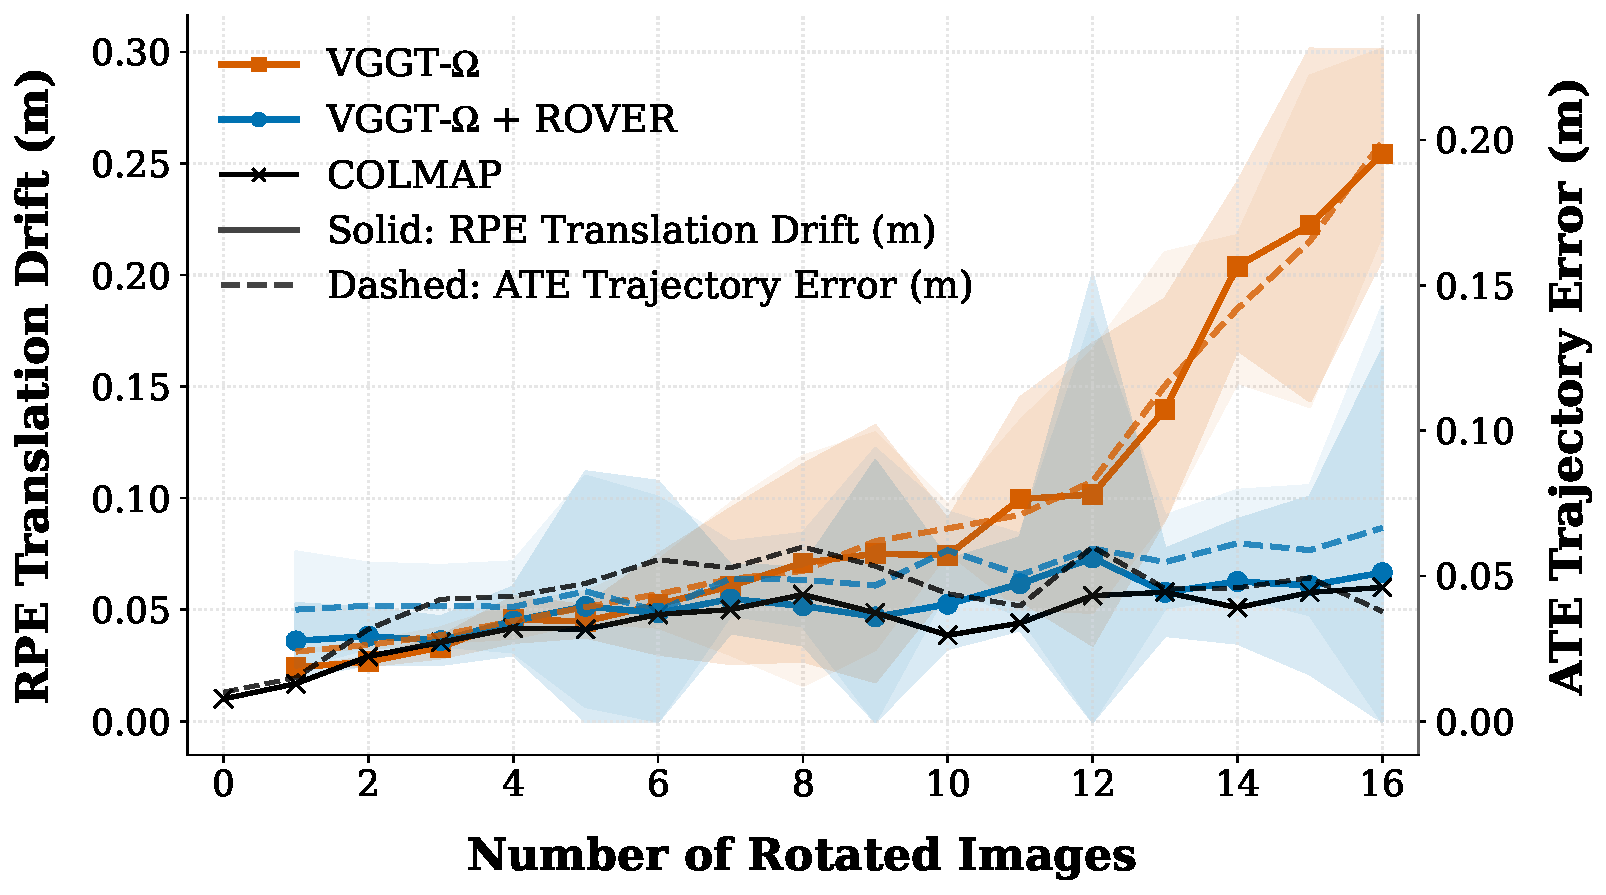
\includegraphics[width=0.75\linewidth]{supplementary_figures/model_comparison.pdf}
    \caption{RPE translation and ATE trajectory error with increasing fraction of rotated input images, comparing ROVER with VGGT-$\Omega$, base model VGGT-$\Omega$ and COLMAP}
    \label{fig:rover_trajectory}
\end{figure}
\subsection{Latency and Computational Overhead of ROVER}
\renewcommand{\arraystretch}{1.2}
\begin{table}[H]
\centering
\small
\setlength{\tabcolsep}{6pt}
\caption{Latency and computational overhead of ROVER across VGGT, VGGT-$\Omega$, $\pi^3$, MapAnything and DepthAnything3}
\label{tab:rover_latency}
\begin{tabular}{lcccc}
\toprule
\textbf{Model} &
\textbf{Base Latency} &
\textbf{ROVER Correction} &
\textbf{Total Latency} &
\textbf{Added Overhead} \\
& \textbf{(seconds)} &
\textbf{(seconds)} &
\textbf{(seconds)} &
\textbf{(\%)} \\
\midrule
VGGT
& \valrow{1.769}{0.017}
& \valrow{0.433}{0.004}
& \valrow{2.169}{0.027}
& $+24.5\%$ \\

VGGT-$\Omega$
& \valrow{1.400}{0.006}
& \valrow{0.424}{0.003}
& \valrow{1.786}{0.009}
& $+30.3\%$ \\

$\pi^3$
& \valrow{1.296}{0.004}
& \valrow{0.428}{0.001}
& \valrow{1.701}{0.034}
& $+33.0\%$ \\

MapA
& \valrow{5.789}{0.038}
& \valrow{0.430}{0.004}
& \valrow{6.203}{0.033}
& $+7.4\%$ \\

DA3
& \valrow{2.003}{0.010}
& \valrow{0.431}{0.003}
& \valrow{2.444}{0.016}
& $+21.5\%$ \\
\bottomrule
\end{tabular}
\end{table}

Additionally we compute latency introduced by the ROVER in ~\Cref{tab:rover_latency} for $16$ images. For all of the models, the introduced latency remains less than $50\%$ of the base model latency, with the observed overhead ranging from $7.4\%$ to $33.0\%$. The ROVER correction itself incurs a nearly constant latency of approximately $0.43$ seconds across all models, irrespective of the underlying model. The relative overhead decreases for models with higher base latency, with Map-Anything incurring only $7.4\%$ overhead, demonstrating the low computational cost of ROVER.


\section{Algorithm}
\label{sec:algorithm}
% ------------------------------------------------------------

% \Badri{All tables should be cited, All sections should be written properly. All tables should be cited in ascending order, meaning if table A is shown before table B and then table A should also be cited before table B }

% \Badri{Fig \Cref{fig:denoise-examples}, the red boxes should be on both colum, also the heading for each row is should be wrriten properly, current all font is small, font style is different. This is very lazy work}

% \Badri{ Fig \Cref{fig:pointcloud_comparison} currently only shows results for vggt, please include results for other models (specially for vggt-omega). They either can be same scene but different models (like in main paper) or can be different scenes as well}

\renewcommand{\algorithmicrequire}{\textbf{Input:}}
\renewcommand{\algorithmicensure}{\textbf{Output:}}

\begin{algorithm}[!htb]
\caption{Rendering-Based Rotated Image Generation}
\label{alg:rotation_generation}
\begin{algorithmic}[1]
    \REQUIRE Multi-view images $\{\mathbf{I}_i\}$, poses $\{\mathbf{P}_i\}$, quality threshold $\tau$
    \ENSURE Rotated images $\{\mathbf{I}_i^{\theta_i}\}$
    \STATE Fit 3DGS representation $\mathcal{G}$ on $\{\mathbf{I}_i, \mathbf{P}_i\}$
           % \COMMENT{Assess reconstruction quality}
    \FOR{each view $i$}
        \STATE Sample $\theta_i \sim \mathcal{U}(0^\circ, 360^\circ)$
        \STATE Compute $\mathbf{P}_i^{\theta_i}$
        \STATE $\mathbf{I}_i^{\theta_i} \leftarrow \mathrm{Render}(\hat{\mathcal{G}},\, \mathbf{P}_i^{\theta_i})$
        \STATE $q \leftarrow \mathrm{VisualQuality\text{-}R1}(\mathbf{I}_i^{\theta_i})$
        \IF{$q \leq \tau$}
            \STATE $\mathbf{I}_i^{\theta_i} \leftarrow \mathrm{Difix3D\_Denoise}(\mathbf{I}_i^{\theta_i})$  \IF{$\mathrm{VisualQuality\text{-}R1}(\mathbf{I}_i^{\theta_i}) \leq \tau$}
                \STATE Exclude view $i$ from evaluation
            \ENDIF
        \ENDIF
    \ENDFOR
    \FOR{each image $\mathbf{I} \in \{\mathbf{I}_i^{\theta_i}\}$}
        \STATE Manually verify $\mathbf{I}$ and remove it from the set if visible artifacts are observed
    \ENDFOR
\end{algorithmic}
\end{algorithm}

\begin{algorithm}[!htb]
\caption{ROVER: Variance-based Canonical Orientation Estimation}
\label{alg:var_alg}
\begin{algorithmic}[1]
    \REQUIRE Image $\mathbf{I}$, frozen DINOv2 encoder $\phi$, 
             coarse step $\Delta_c = 15^\circ$, fine window 
             $\Delta_f = 7^\circ$
    \ENSURE Canonicalized image $\mathbf{I}^{\mathrm{can}}$ 
            with estimated roll $\hat{\theta}$

    \STATE \textit{// Coarse stage}
    \STATE $\Theta_\text{coarse} \leftarrow 
           \{k \cdot \Delta_c \mid k = 1, \ldots, 
           \lfloor 360^\circ / \Delta_c \rfloor\}$
    \FOR{each $\theta \in \Theta_\text{coarse}$}
        \STATE $V(\theta) \leftarrow \textsc{EmbedVar}^{\ref{alg:embedvar}}
               (\mathbf{I}, \theta, \phi)$
    \ENDFOR
    \STATE $\theta_c \leftarrow 
           \arg\max_{\theta \in \Theta_\text{coarse}} V(\theta)$

    \STATE \textit{// Fine stage}
    \STATE $\Theta_\text{fine} \leftarrow 
           \{\theta_c + \delta \mid \delta \in 
           [-\Delta_f, \Delta_f],\, \delta \in \mathbb{Z}\}$
    \FOR{each $\theta \in \Theta_\text{fine}$}
        \STATE $V(\theta) \leftarrow \textsc{EmbedVar}^{\ref{alg:embedvar}}
               (\mathbf{I}, \theta, \phi)$
    \ENDFOR
    \STATE $\hat{\theta} \leftarrow 
           \arg\max_{\theta \in \Theta_\text{fine}} V(\theta)$

    \STATE \textit{// Canonicalization}
    \STATE $\mathbf{I}^{\mathrm{can}} \leftarrow 
           \mathrm{Rotate}(\mathbf{I},\, -\hat{\theta})$
    \RETURN $\mathbf{I}^{\mathrm{can}},\, \hat{\theta}$
\end{algorithmic}
\end{algorithm}

\begin{algorithm}[!htb]
\caption{\textsc{EmbedVar}: Patch Embedding Variance Computation}
\label{alg:embedvar}
\begin{algorithmic}[1]
    \REQUIRE Image $\mathbf{I}$, candidate orientation $\theta$, 
             frozen DINOv2 encoder $\phi$
    \ENSURE Patch embedding variance $V(\theta)$
    \STATE $\mathbf{Z}_\theta \leftarrow 
           \phi(\mathrm{Rotate}(\mathbf{I}, \theta))$
           \COMMENT{$M$ patch embeddings $\in \mathbb{R}^D$}
    \STATE $\bar{\mathbf{z}}^\theta \leftarrow 
           \frac{1}{M}\sum_{j=1}^{M} \mathbf{z}_j^\theta$
           \COMMENT{Mean patch embedding}
    \RETURN $\frac{1}{M}\sum_{j=1}^{M}
            \|\mathbf{z}_j^\theta - 
            \bar{\mathbf{z}}^\theta\|_2^2$
\end{algorithmic}
\end{algorithm}


% \begin{algorithm}[H]
% \caption{Variance-based angle detection}
% \label{alg:var_alg}
% \begin{algorithmic}[1]
%     \REQUIRE Image $\mathbf{I}$, candidate orientation set $\Theta$, frozen DINOv2 encoder $\phi$
%     \ENSURE Rotated image $\mathbf{I}^{\theta^\star}$ with predicted roll $\theta^\star$
%     \FOR{each candidate orientation $\theta \in \Theta$}
%         \STATE $\mathbf{I}^{\theta} \leftarrow \mathrm{Rotate}(\mathbf{I},\, \theta)$
%         \STATE $\mathbf{Z}_{\theta} \leftarrow \phi(\mathbf{I}^{\theta})
%                = \{\mathbf{z}_1^\theta, \ldots, \mathbf{z}_M^\theta\}$
%                \COMMENT{Patch embeddings, $\mathbf{z}_j^\theta \in \mathbb{R}^D$}
%         \STATE $\bar{\mathbf{z}}^\theta \leftarrow
%                \frac{1}{M}\sum_{j=1}^{M} \mathbf{z}_j^\theta$
%                \COMMENT{Embedding centroid}
%         \STATE $V(\theta) \leftarrow
%                \frac{1}{M}\sum_{j=1}^{M}
%                \bigl\|\mathbf{z}_j^\theta - \bar{\mathbf{z}}^\theta\bigr\|_2^2$
%                \COMMENT{Patch-embedding variance}
%     \ENDFOR
%     \STATE $\theta^\star \leftarrow \arg\max_{\theta \in \Theta} V(\theta)$
%     \RETURN $\mathbf{I}^{\theta^\star},\, \theta^\star$
% \end{algorithmic}
% \end{algorithm}


% \begin{algorithm}[H]
% \caption{ROVER: Variance-based Canonical Orientation Estimation}
% \label{alg:var_alg}
% \begin{algorithmic}[1]
%     \REQUIRE Image $\mathbf{I}$, frozen DINOv2 encoder $\phi$, 
%              coarse step $\Delta_c = 15^\circ$, fine window 
%              $\Delta_f = 7^\circ$
%     \ENSURE Canonicalized image $\mathbf{I}^{\mathrm{can}}$ 
%             with estimated roll $\hat{\theta}$

%     \STATE \textit{// Coarse stage}
%     \STATE $\Theta_\text{coarse} \leftarrow 
%            \{k \cdot \Delta_c \mid k = 1, \ldots, 
%            \lfloor 360^\circ / \Delta_c \rfloor\}$
%     \FOR{each $\theta \in \Theta_\text{coarse}$}
%         \STATE $V(\theta) \leftarrow \textsc{EmbedVar}
%                (\mathbf{I}, \theta, \phi)$
%     \ENDFOR
%     \STATE $\theta_c \leftarrow 
%            \arg\max_{\theta \in \Theta_\text{coarse}} V(\theta)$

%     \STATE \textit{// Fine stage}
%     \STATE $\Theta_\text{fine} \leftarrow 
%            \{\theta_c + \delta \mid \delta \in 
%            [-\Delta_f, \Delta_f],\, \delta \in \mathbb{Z}\}$
%     \FOR{each $\theta \in \Theta_\text{fine}$}
%         \STATE $V(\theta) \leftarrow \textsc{EmbedVar}
%                (\mathbf{I}, \theta, \phi)$
%     \ENDFOR
%     \STATE $\hat{\theta} \leftarrow 
%            \arg\max_{\theta \in \Theta_\text{fine}} V(\theta)$

%     \STATE \textit{// Canonicalization}
%     \STATE $\mathbf{I}^{\mathrm{can}} \leftarrow 
%            \mathrm{Rotate}(\mathbf{I},\, -\hat{\theta})$
%     \RETURN $\mathbf{I}^{\mathrm{can}},\, \hat{\theta}$
% \end{algorithmic}
% \end{algorithm}


% \begin{algorithm}[H]
% \caption{\textsc{EmbedVar}: Patch Embedding Variance Computation}
% \label{alg:embedvar}
% \begin{algorithmic}[1]
%     \REQUIRE Image $\mathbf{I}$, candidate orientation $\theta$, 
%              frozen DINOv2 encoder $\phi$
%     \ENSURE Patch embedding variance $V(\theta)$
%     \STATE $\mathbf{Z}_\theta \leftarrow 
%            \phi(\mathrm{Rotate}(\mathbf{I}, \theta))$
%            \COMMENT{$M$ patch embeddings $\in \mathbb{R}^D$}
%     \STATE $\bar{\mathbf{z}}^\theta \leftarrow 
%            \frac{1}{M}\sum_{j=1}^{M} \mathbf{z}_j^\theta$
%            \COMMENT{Mean patch embedding}
%     \RETURN $\frac{1}{M}\sum_{j=1}^{M}
%             \|\mathbf{z}_j^\theta - 
%             \bar{\mathbf{z}}^\theta\|_2^2$
% \end{algorithmic}
% \end{algorithm}


Algorithm~\Cref{alg:rotation_generation} provides the pseudocode for controlled rotation synthesis. We first fit a 3DGS representation to each multi-view captured image set. We then sample an angle $\theta \sim \mathcal{U}(0^\circ, 360^\circ)$, render the corresponding rolled image, and score its reconstruction quality $q$ with VisualQuality-R1 \citep{wu2026visualquality}. Captures falling below the predefined threshold $\tau$ are denoised with Difix3D single-step denoiser to remove artifacts, after which the remaining scenes are rendered directly. The renderings are scored again with reconstruction quality $q$ with VisualQuality-R1 to remove images with obvious artifacts. A final manual pass removes images with any residual artifacts.
Orientation is then recovered through (Algorithm~\Cref{alg:var_alg}). For every candidate orientation $\theta\in\Theta$ in a predefined discrete set $\Theta=\{0^\circ,\delta,\ldots,360^\circ-\delta\}$, the input image is rotated by $\theta$ and passed through the frozen DINOv2 encoder $\phi$ to obtain the corresponding patch embeddings,
$\mathbf{Z}_{\theta}=\phi(\mathbf{I}^{\theta})=\{\mathbf{z}_1^\theta,\mathbf{z}_2^\theta,\ldots,\mathbf{z}_M^\theta\}$,
where $\mathbf{I}^{\theta}$ denotes the image rotated by $\theta$, and $\mathbf{z}_j^\theta\in\mathbb{R}^D$ denotes the embedding corresponding to the $j$-th image patch. Each candidate orientation is scored by the variance of its patch embeddings about their centroid,
$V(\theta)=\frac{1}{M}\sum_{j=1}^{M}\left\|\mathbf{z}_j^\theta-\bar{\mathbf{z}}^\theta\right\|_2^2$,
where $\bar{\mathbf{z}}^\theta=\frac{1}{M}\sum_{j=1}^{M}\mathbf{z}_j^\theta$ is the centroid of the patch embeddings. Since the backbone is pre-trained predominantly on upright imagery, patch features are most strongly differentiated at the canonical orientation and collapse toward the centroid as the rotation departs from it. The orientation estimation operator is therefore defined as
$
E(\mathbf{I})=\arg\max_{\theta\in\Theta}V(\theta),
$
and the maximizing candidate gives the predicted roll. We use DINOv2 embeddings to determine the canonical orientation in our approach. Previous works \citep{cuttano2026insid3} points out that DINOv3 features can exhibit spurious correspondences between image pairs regardless of their semantic similarity. In particular, feature similarities between semantically unrelated images exhibit systematic activations aligned with absolute spatial coordinates, indicating a strong positional bias. This positional bias in DINOv3 hinders its ability to accurately identify canonical rotation angle using our variance-maximization approach which makes DINOv2 as an encoder $\phi$.

\section{Orientation Variance Plots}
\label{sec:ROVER_empirical_plots}

We include plot of variance of token embeddings w.r.t. the image orientation in \cref{fig:variance_vs_angle_all_datasets} for datasets 7-Scenes, NRGB-D, Tanks and Temples and RotMV. To analyze the orientation dependence of DINOv2 representations, we synthetically rotate each canonical image over \(0^\circ\!-\!360^\circ\) in \(15^\circ\) increments and compute the same patch-token spatial variance used by our method, excluding padded regions introduced by rotation. To isolate orientation-dependent changes from image-specific differences in absolute variance, each image’s variance curve is independently min–max normalized across candidate rotations before aggregation. 

\Cref{fig:variance_vs_angle_all_datasets} shows the mean normalized variance across all images, with \(\pm 1\) standard deviation. We use upright images here to calculate variance. We show that for all datasets, the variance of token embeddings consistently achieves its maximum value at canonical orientation ($0^\circ$ in this case, as we used upright images), while non-canonical rotations produce substantially lower values with weaker secondary peaks near multiples of \(90^\circ\). This supports the use of DINOv2 patch-embedding variance as a reliable signal for identifying canonical upright orientation. 


\begin{figure*}[!ht]
    \centering
    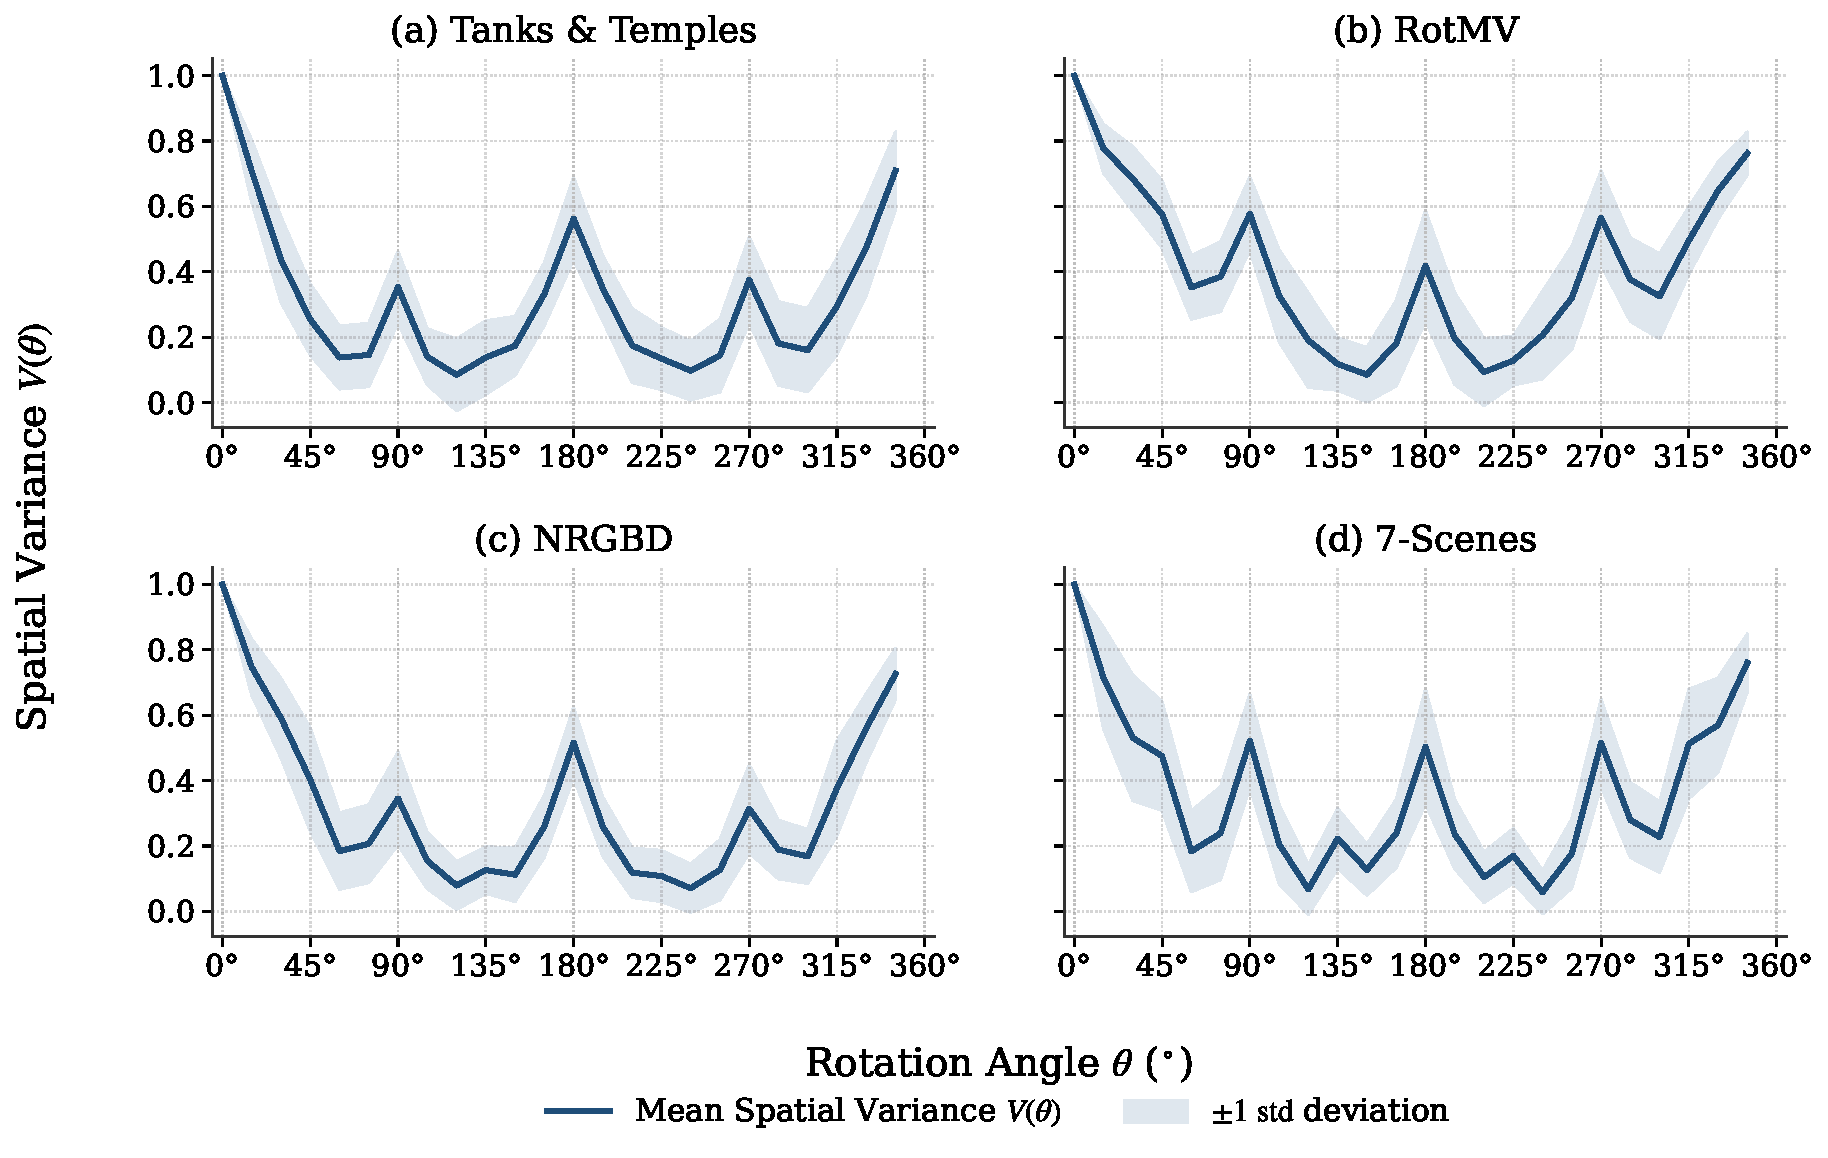
\includegraphics[width=0.98\textwidth]{supplementary_figures/variance_plots/all_datasets_grid_2x2.pdf}
    \caption{
        Variance as a function of rotation angle across the RotMV, NRGB-D, 7-Scenes, and Tanks and Temples datasets. We observe that ROVER consistently helps estimate the upright orientation of the images 
    }
    \label{fig:variance_vs_angle_all_datasets}
\end{figure*}
We also plot the variance for images rotated by $225^\circ$ in \cref{fig:variance_vs_angle_225_deg} for Tanks and Temples, NRGB-D and 7-Scenes. Each rotated image is further rotated by candidate angles over $[0^\circ, 360^\circ)$ in $15^\circ$ increments, and the variance is maximized by the candidate that restores the upright orientation ($135^\circ$). We plot the mean normalized variance against the estimated rotation $\theta = 360^\circ - $ candidate, so the peak appears at $\theta = 225^\circ$ for all three datasets and the correction is simply a rotation by $-\theta$. In the upright setting, the peak occurs at $0^\circ$, where no rotation (and hence no padding) is applied, so one could argue the peak is simply caused by the absence of padding. Here, leaving the image unrotated ($\phi = 0^\circ$) does not give the maximum; instead, the peak occurs at $\phi = 135^\circ$, which adds padding(because of the rotation) but restores the upright view. This shows that the variance peak is driven by the upright orientation of the image content, not by the padding.

\begin{figure*}[!ht]
    \centering
    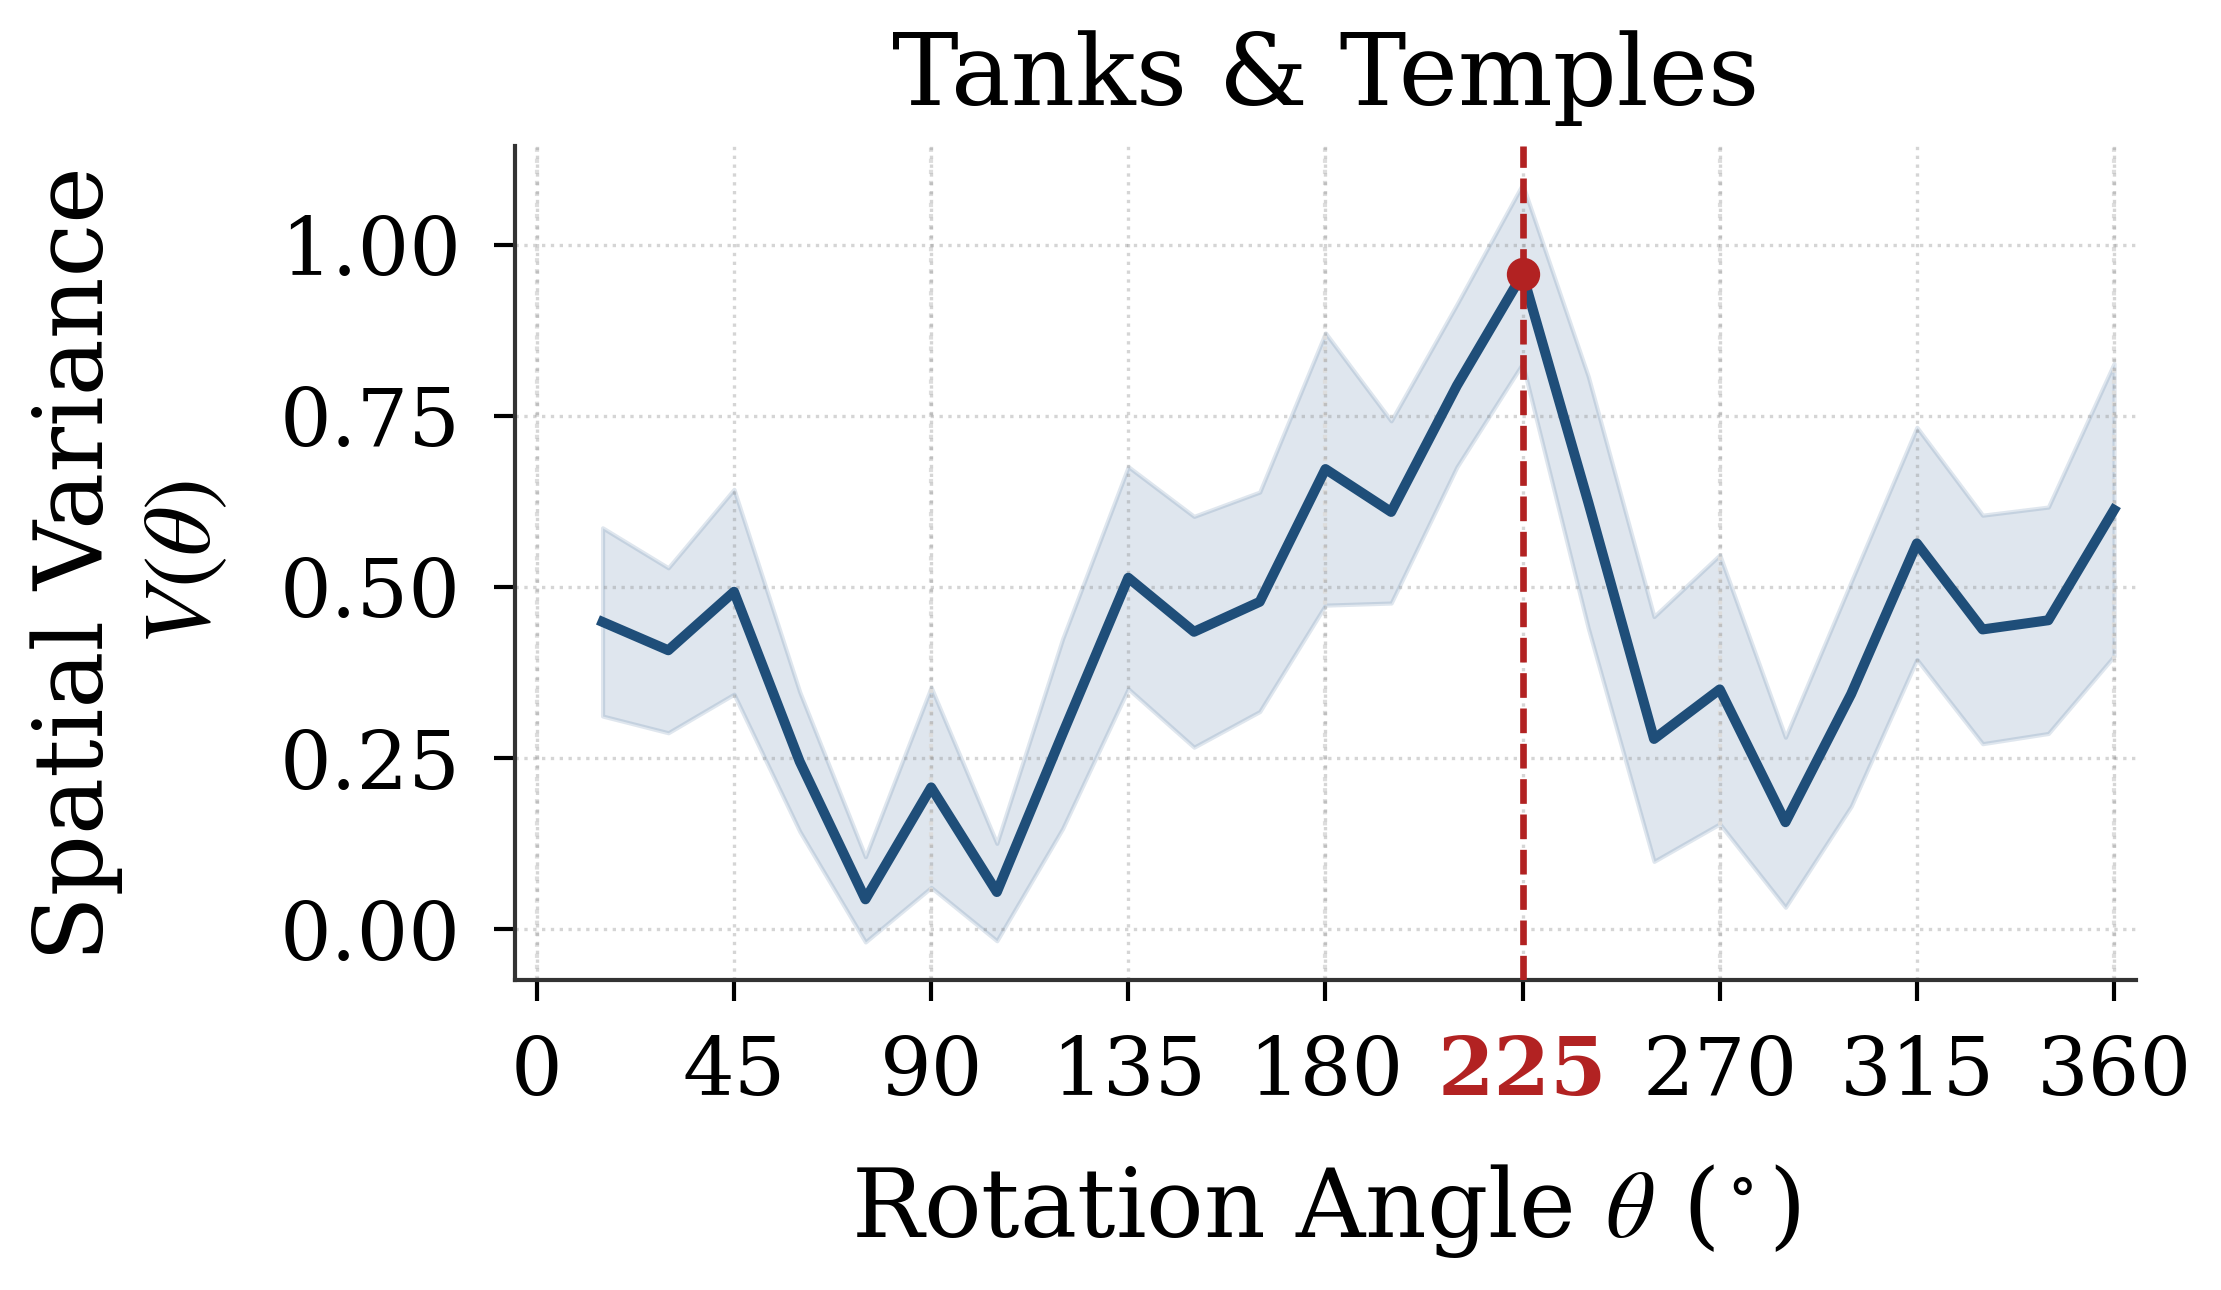
\includegraphics[width=0.325\textwidth]{supplementary_figures/variance_plots/all_scenes_variance_vs_angle_tnt_225.png}\hfill
    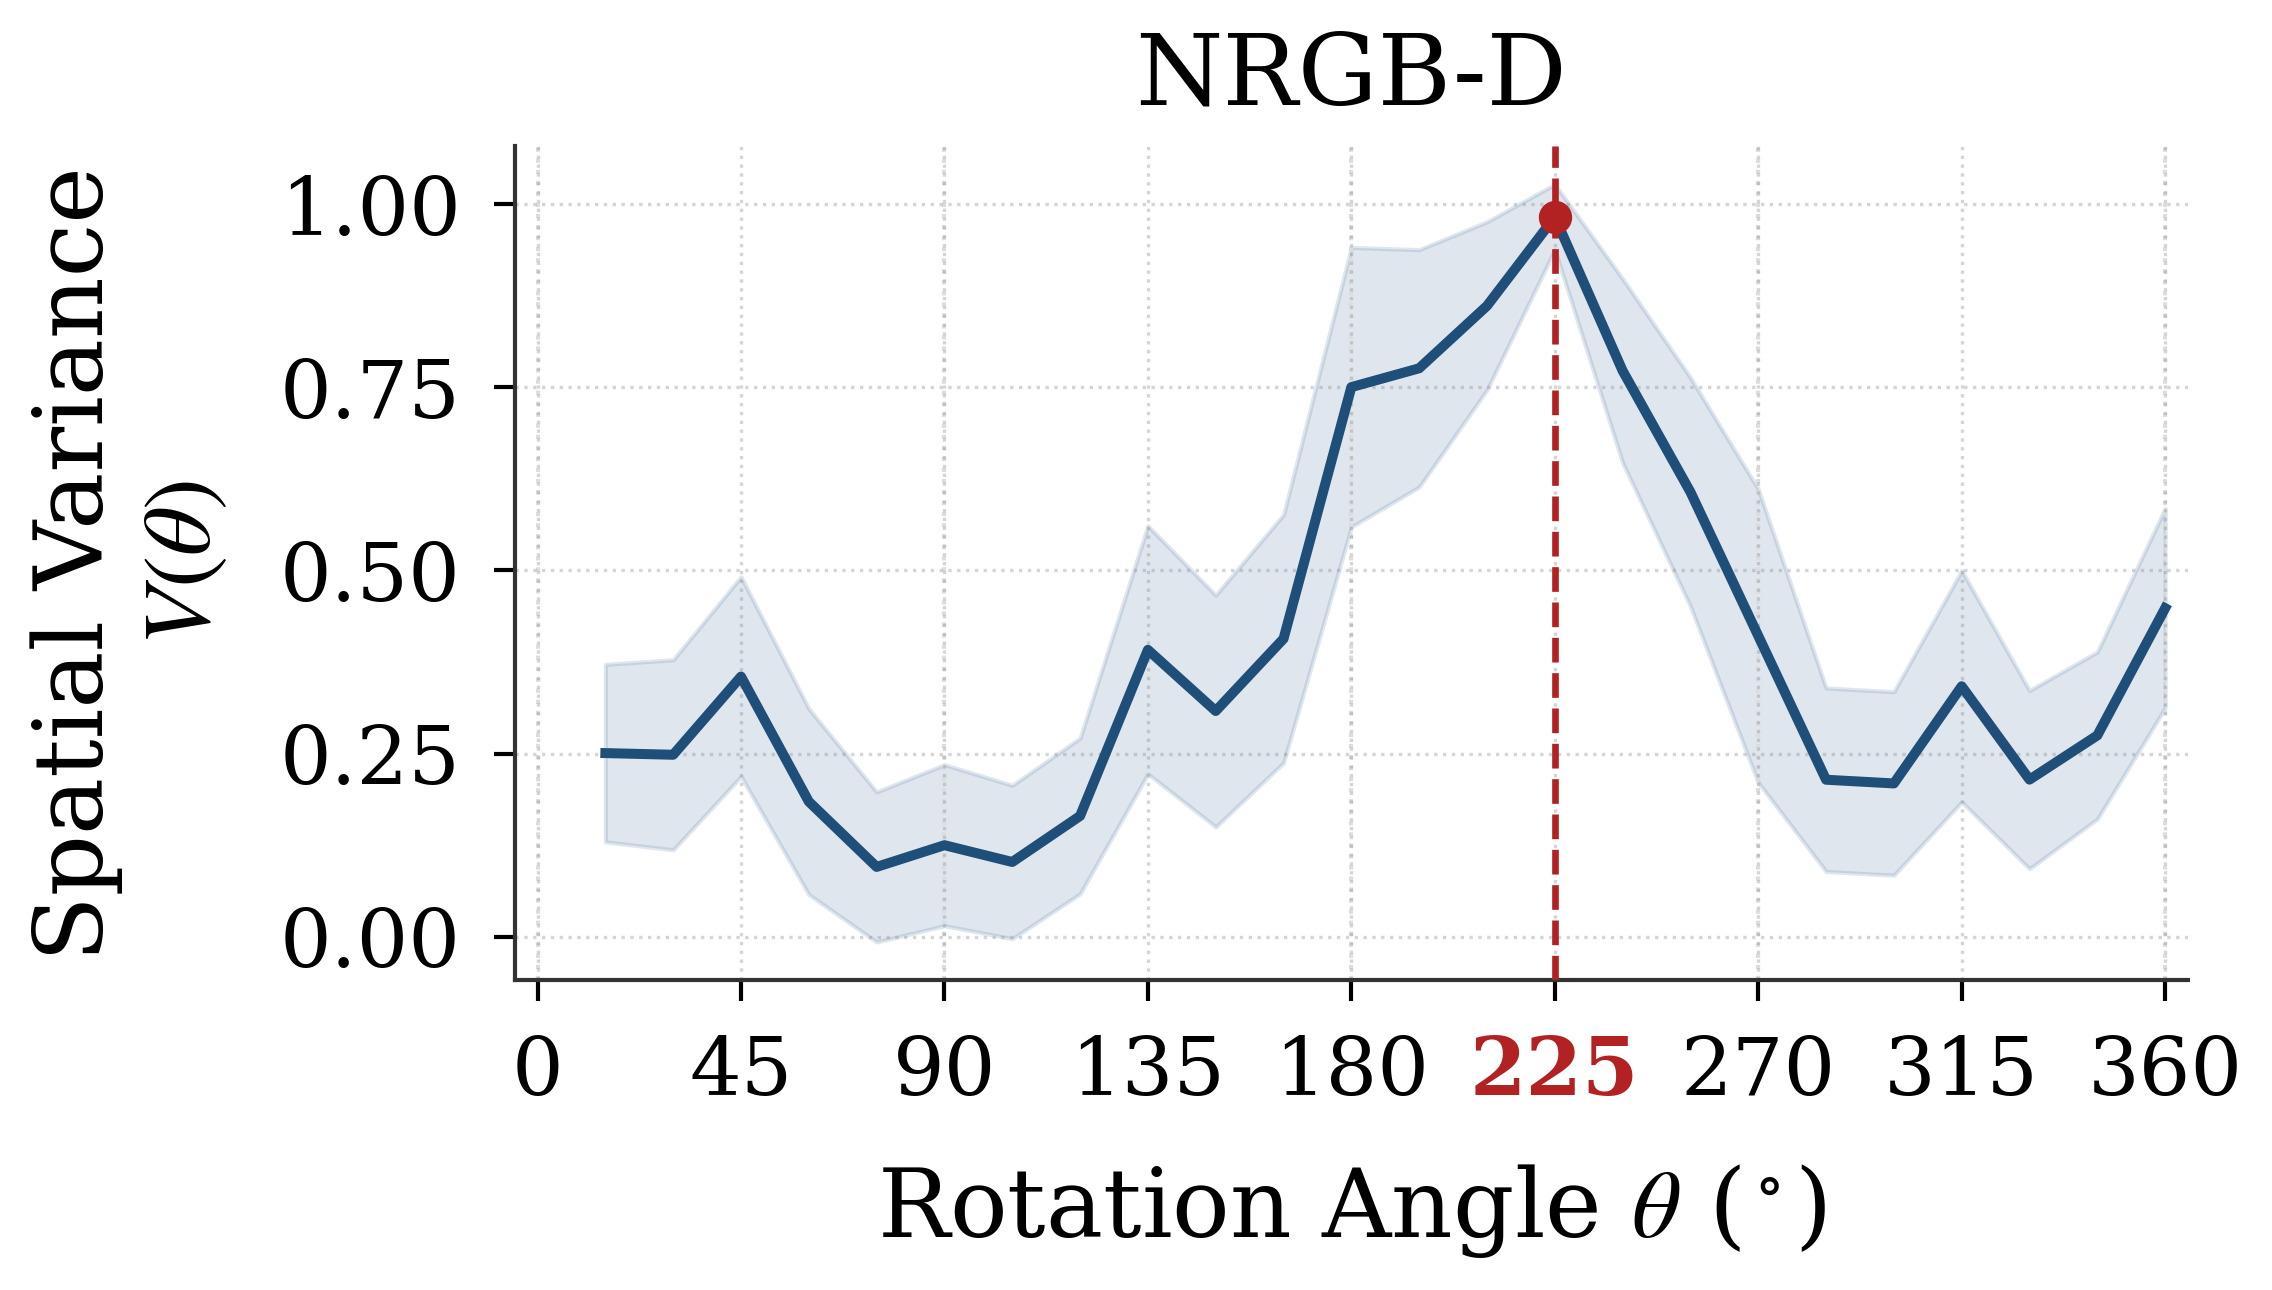
\includegraphics[width=0.325\textwidth]{supplementary_figures/variance_plots/all_scenes_variance_vs_angle_nrgbd.png}\hfill
    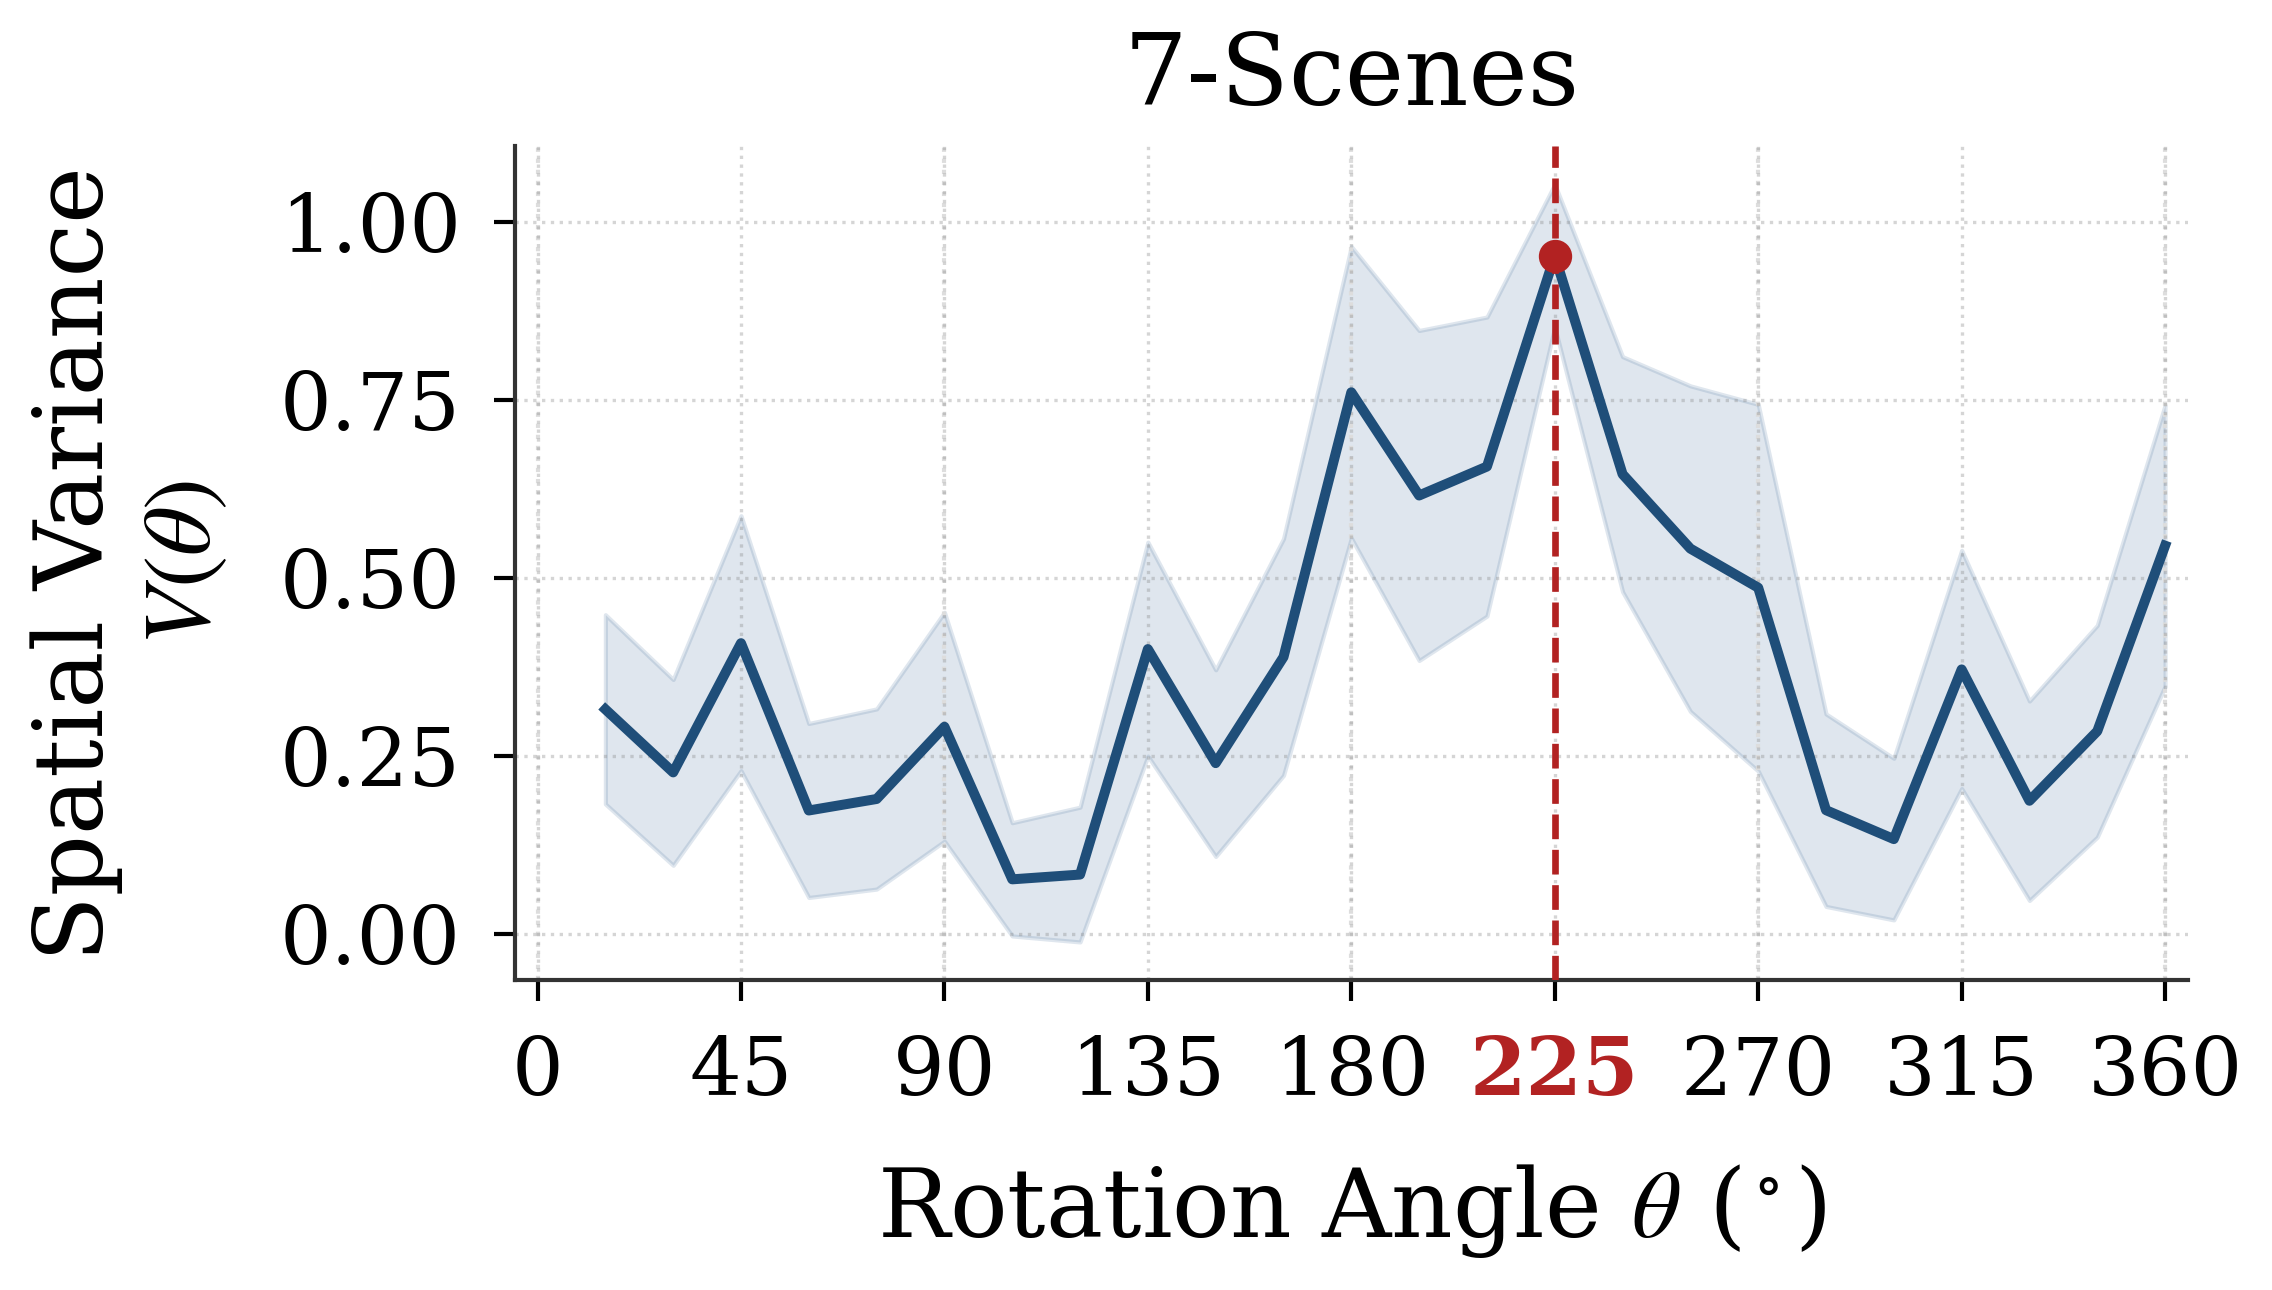
\includegraphics[width=0.325\textwidth]{supplementary_figures/variance_plots/all_scenes_variance_vs_angle_7scenes_225.png}
\caption{ROVER recovers the true rotation angle. Input images are rotated by $225^\circ$ from their upright orientation. We plot the normalized patch-embedding variance (mean $\pm 1$ std) against the estimated rotation $\theta = 360^\circ - \phi$, where $\phi$ is the candidate correction. The peak (red dashed line) falls at $\theta = 225^\circ$ for all three datasets, so rotating by $-\theta$ restores the upright view.}
    \label{fig:variance_vs_angle_225_deg}
\end{figure*}

% ------------------------------------------------------------
\section{Sensitivity to Limited Pitch Rotations}  % TODO: rename
\label{sec:pose_pitch}
% ------------------------------------------------------------
We additionally evaluate sensitivity to camera rotations about the pitch axis on NRGB-D, 7-Scenes, and Tanks\&Temples in~\Cref{tab:pitch_metrics}. Following the evaluation protocol described in~\Cref{sec:experimental_setup}, we evaluate the four non-zero rotation levels ($25\%$, $50\%$, $75\%$, and $100\%$ rotated views). Selected views are independently assigned a pitch perturbation from $[-5^\circ, +5^\circ]$; the corresponding camera pose is then perturbed and a new view is rendered using~\Cref{sec:rendering_based_rotation}. Large perturbation leads to change in viewpoint of the scene as the camera will point to a different region in the scene unlike roll perturbation thus we restrict the perturbation to limited range. Across this limited range, performance remains close to the upright setting for most models and datasets. For instance, VGGT changes from $0.798$ to $0.796$ N.C. and from $98.36$ to $98.17$ AUC$_{30}$ on NRGB-D, while on Tanks\&Temples the corresponding values change from $0.678$ to $0.671$ and from $91.62$ to $91.20$. Larger variation is observed in some cases, such as $\pi^3$ on Tanks\&Temples, where N.C. decreases from $0.701$ to $0.666$, although pose accuracy remains comparatively stable. Overall, these results indicate sensitivity to small pitch perturbations over the evaluated range.

\renewcommand{\arraystretch}{1.2}
\providecommand{\dd}[2]{\makecell{#1 \\ {\tiny $\pm$ #2}}}

\begin{table}[h]
\centering
\caption{Point-map (N.C., $\uparrow$) and pose (AUC@30, $\uparrow$) accuracy, upright vs.\ rotated about the pitch axis, on NRGBD, 7-Scenes, and Tanks\&Temples.}
\label{tab:pitch_metrics}
\scriptsize
\setlength{\tabcolsep}{3pt}
\resizebox{\linewidth}{!}{%
\begin{tabular}{l *{3}{cc cc}}
\toprule
 & \multicolumn{4}{c}{\textbf{NRGBD}}
 & \multicolumn{4}{c}{\textbf{7-Scenes}}
 & \multicolumn{4}{c}{\textbf{Tanks\&Temples}} \\
\cmidrule(lr){2-5} \cmidrule(lr){6-9} \cmidrule(lr){10-13}

 & \multicolumn{2}{c}{N.C. $\uparrow$}
 & \multicolumn{2}{c}{AUC@30 $\uparrow$}
 & \multicolumn{2}{c}{N.C. $\uparrow$}
 & \multicolumn{2}{c}{AUC@30 $\uparrow$}
 & \multicolumn{2}{c}{N.C. $\uparrow$}
 & \multicolumn{2}{c}{AUC@30 $\uparrow$} \\
\cmidrule(lr){2-3} \cmidrule(lr){4-5}
\cmidrule(lr){6-7} \cmidrule(lr){8-9}
\cmidrule(lr){10-11} \cmidrule(lr){12-13}

\textbf{Method}
& Up. & Rot. & Up. & Rot.
& Up. & Rot. & Up. & Rot.
& Up. & Rot. & Up. & Rot. \\
\midrule

VGGT
& \dd{0.798}{0.031} & \dd{0.796}{0.005} & \dd{98.36}{1.44} & \dd{98.17}{0.38}
& \dd{0.661}{0.038} & \dd{0.662}{0.003} & \dd{85.60}{6.73} & \dd{84.68}{1.23}
& \dd{0.678}{0.054} & \dd{0.671}{0.022} & \dd{91.62}{14.60} & \dd{91.20}{0.79} \\
\addlinespace[3pt]

VGGT-$\Omega$
& \dd{0.827}{0.049} & \dd{0.824}{0.007} & \dd{99.22}{0.57} & \dd{98.84}{0.43}
& \dd{0.670}{0.050} & \dd{0.670}{0.003} & \dd{88.07}{5.80} & \dd{87.05}{1.20}
& \dd{0.684}{0.083} & \dd{0.664}{0.016} & \dd{92.88}{14.29} & \dd{92.79}{0.36} \\
\addlinespace[3pt]

$\pi^3$
& \dd{0.807}{0.077} & \dd{0.805}{0.007} & \dd{96.32}{2.74} & \dd{95.86}{0.56}
& \dd{0.682}{0.050} & \dd{0.683}{0.003} & \dd{85.13}{8.09} & \dd{84.59}{1.36}
& \dd{0.701}{0.056} & \dd{0.666}{0.030} & \dd{94.46}{8.71} & \dd{94.20}{0.86} \\
\addlinespace[3pt]

MapA.
& \dd{0.741}{0.052} & \dd{0.720}{0.012} & \dd{93.86}{3.79} & \dd{93.25}{0.84}
& \dd{0.631}{0.059} & \dd{0.633}{0.010} & \dd{76.22}{15.42} & \dd{75.69}{1.82}
& \dd{0.614}{0.065} & \dd{0.592}{0.030} & \dd{92.48}{3.04} & \dd{91.70}{1.29} \\
\addlinespace[3pt]

DA3
& \dd{0.815}{0.043} & \dd{0.810}{0.009} & \dd{99.77}{0.37} & \dd{99.74}{0.11}
& \dd{0.678}{0.041} & \dd{0.678}{0.004} & \dd{88.14}{5.95} & \dd{87.44}{1.48}
& \dd{0.694}{0.057} & \dd{0.683}{0.024} & \dd{98.45}{1.16} & \dd{97.87}{1.83} \\

\bottomrule
\end{tabular}%
}
\end{table}

\section{Examples of Point Cloud Degradation}

% \Badri{Add additinoal results where we show degradation when all images are rotated with same angle}
We qualitatively illustrate the effect of in-plane roll on point-cloud reconstruction in Figures \Cref{fig:pc_tanks_and_temples}, \Cref{fig:pc_tnt_barn}
\Cref{fig:pc_7scenes_kitchen} 
across VGGT, VGGT-$\Omega$, $\pi^3$, and DepthAnything3 (DA3). Under rotated inputs,
the baseline reconstructions exhibit substantial geometric artifacts, including distorted
structures, misaligned surfaces, and, most prominently, duplicated scene elements, as
highlighted in the zoomed regions. Applying ROVER consistently reduces these artifacts
across the different backbones and produces substantially cleaner and more coherent
point-cloud reconstructions despite the input images being arbitrarily rotated in-plane.

We additionally evaluate the setting where all input images are rotated by the same angle in ~\Cref{fig:uniform_rotation_office}, preserving their relative orientations. Surprisingly, models still fail to reconstruct the scene, demonstrating that the degradation is not caused by relative pose ambiguity between views but by a learned prior on absolute image orientation the model simply does not expect to see images that deviate from upright.

%%%%%%%%%%%%%%%%%%%%%%%%%%%%%%%%%%%%%%%%%%%%%%%%=========================================================================
% PAGE 1: Tanks & Temples (Truck, Church) + 7-Scenes (Office)
% =========================================================================
\begin{figure*}[p]
\centering

% --- Dataset 1: Tanks & Temples ---
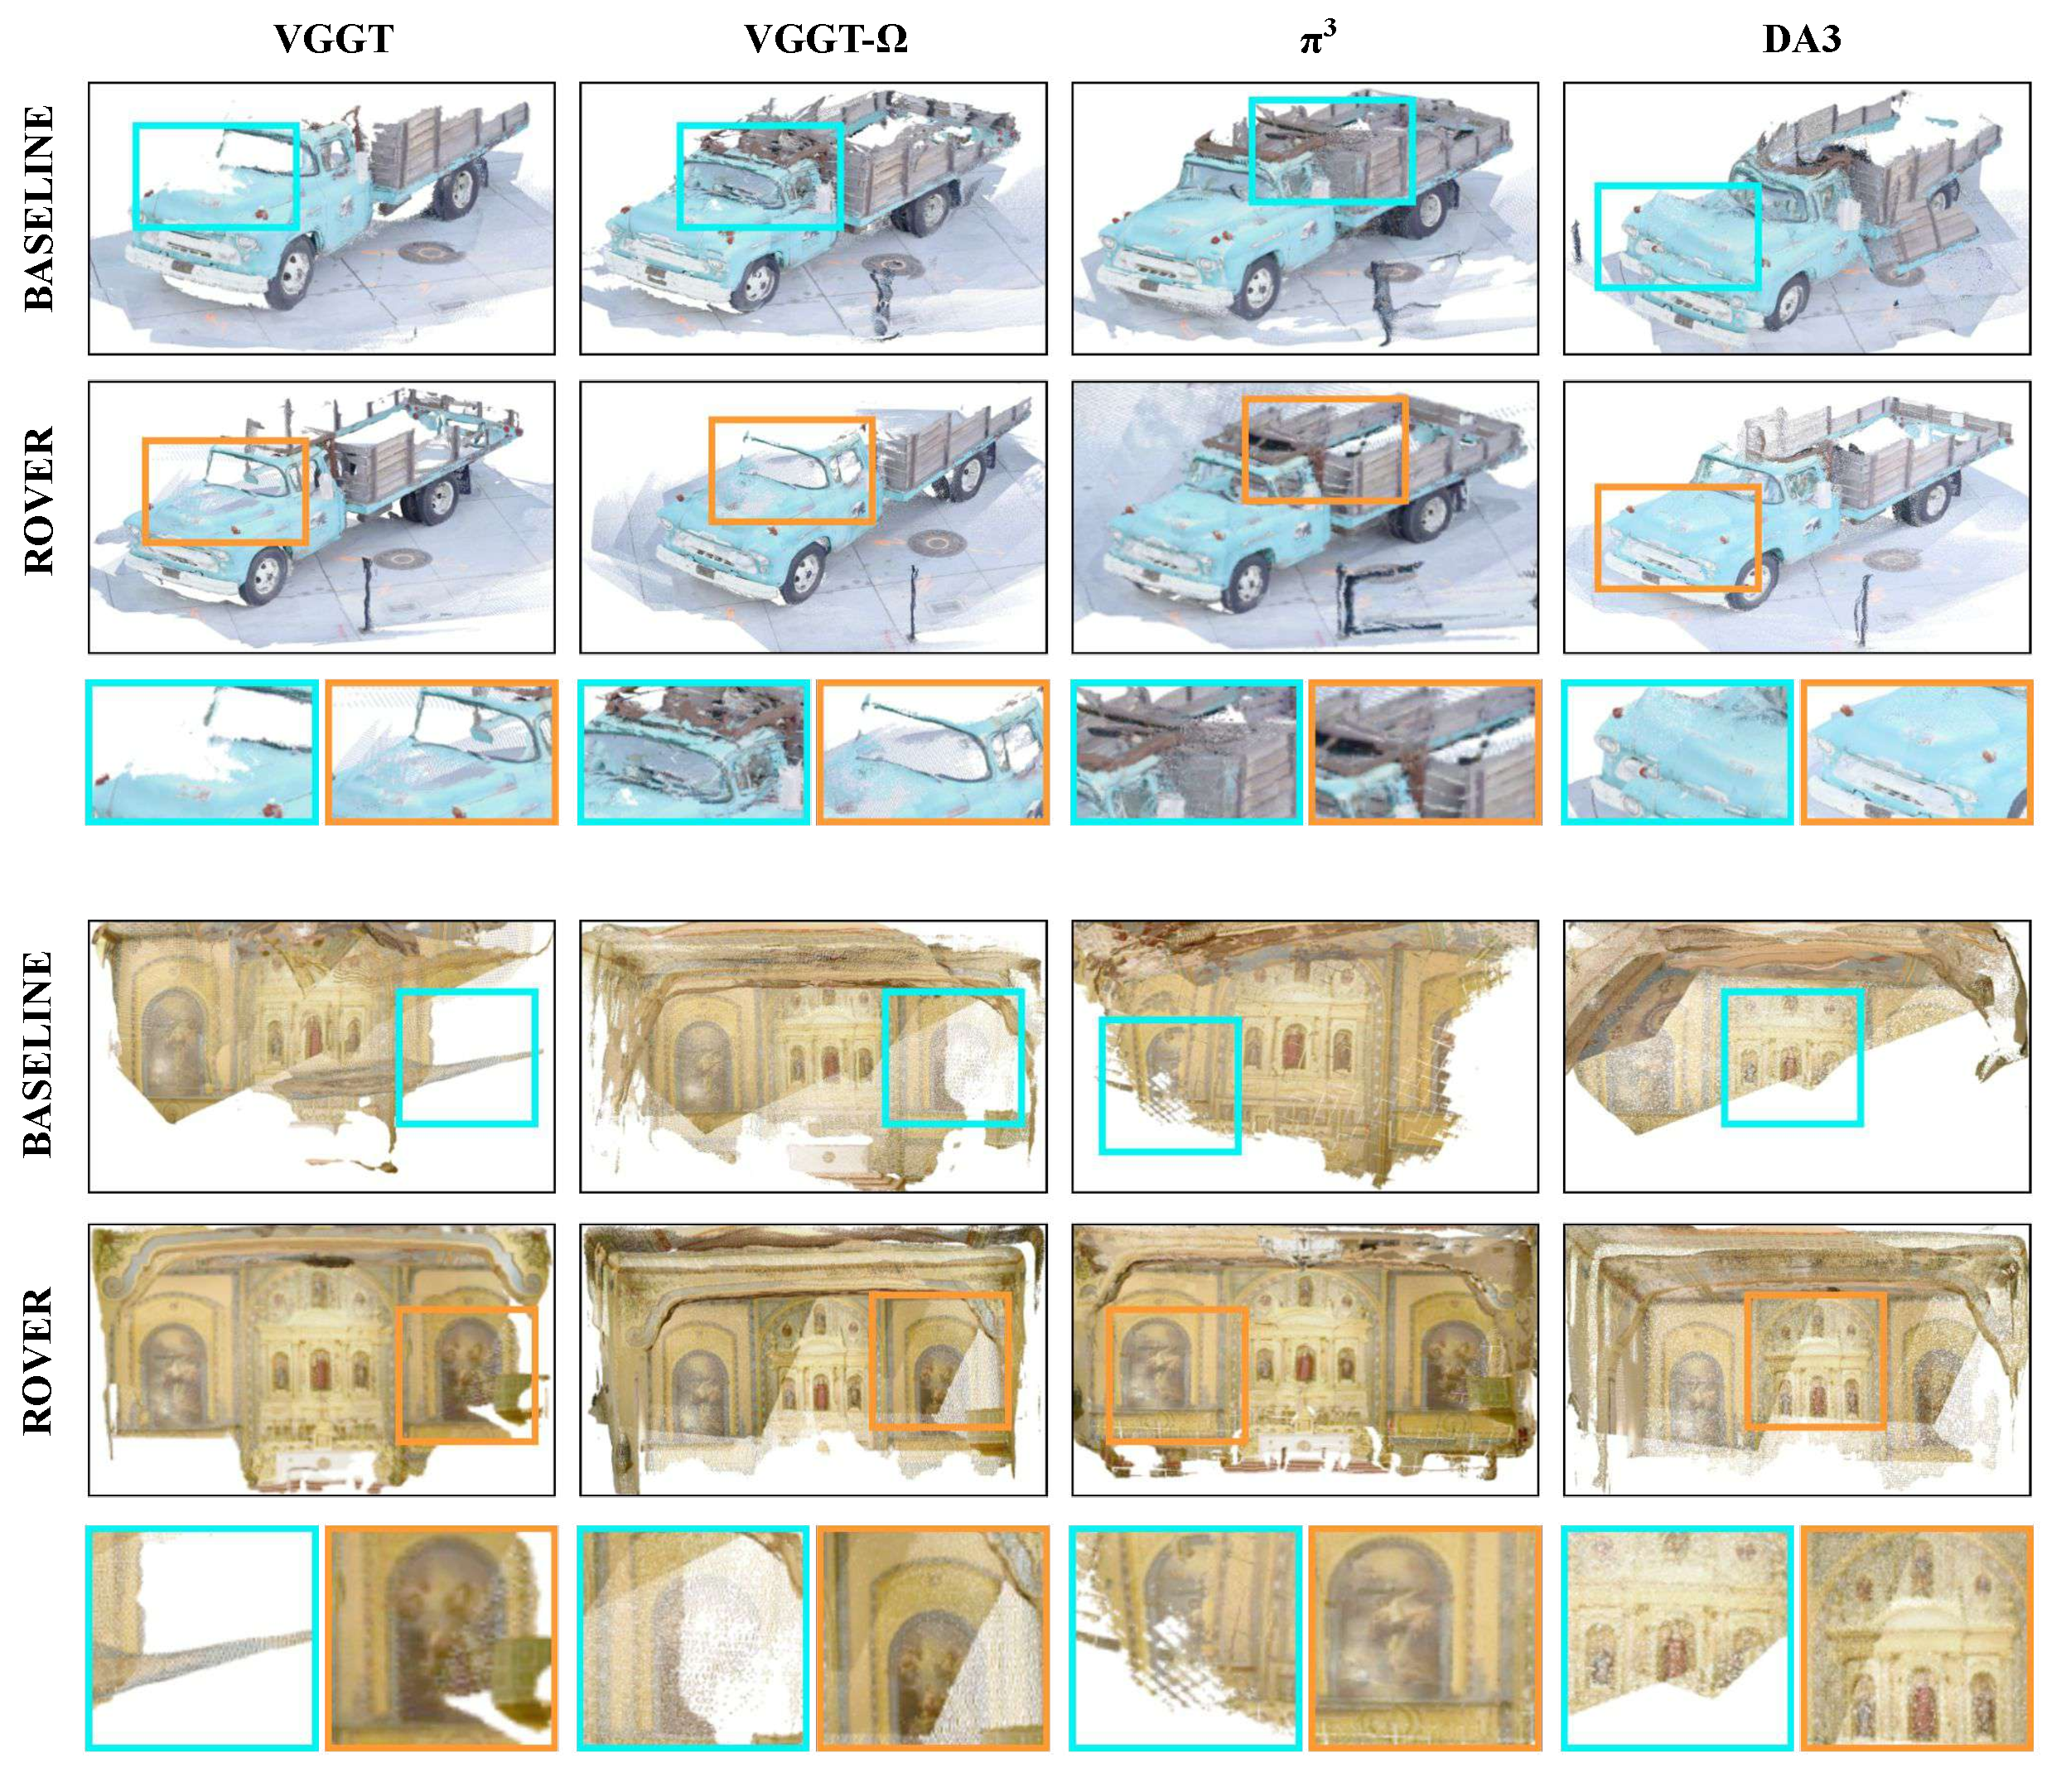
\includegraphics[width=\textwidth]{supplementary_figures/pointcloud_comparisons/supplementary_fig_1.pdf}
\caption{\textbf{Qualitative comparison on the Tanks \& Temples dataset} (Truck and Church scenes). Point cloud reconstructions across VGGT, VGGT-$\Omega$, $\pi^3$, and DA3 comparing baseline and ROVER.}
\label{fig:pc_tanks_and_temples}

\vspace{4mm}

% --- Dataset 2 (Part 1): 7-Scenes (Office) ---
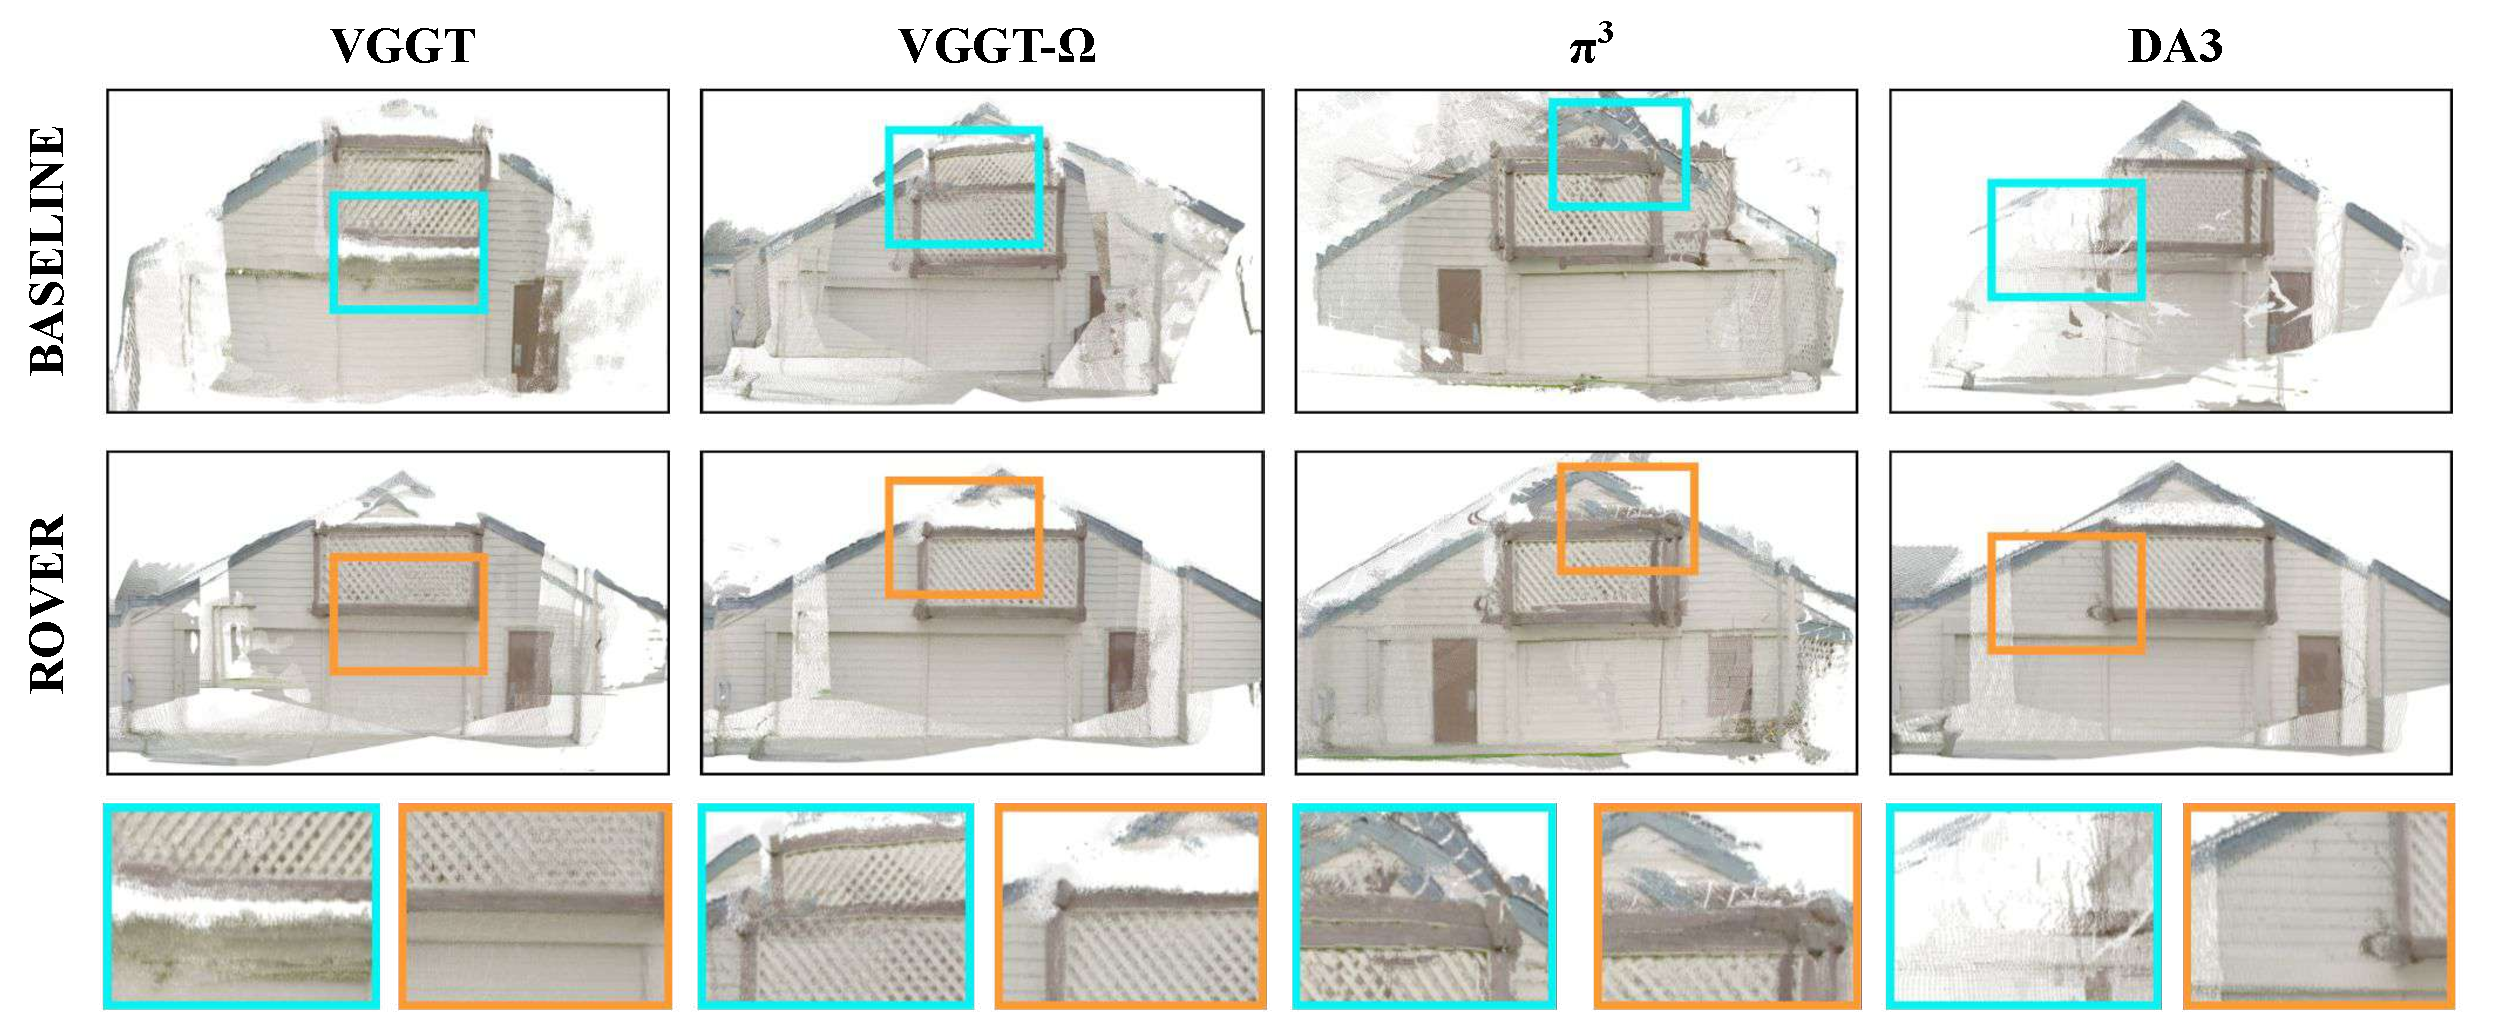
\includegraphics[width=\textwidth]{supplementary_figures/pointcloud_comparisons/supplementary_fig_2.1.pdf}
\caption{\textbf{Qualitative comparison on the Barn scene} from Tanks \& Temples dataset . Reconstruction comparisons across baseline and ROVER settings.}
\label{fig:pc_tnt_barn}

\end{figure*}


% \clearpage % Pushes the next figure onto its own new page

% =========================================================================
% PAGE 2: 7-Scenes (Kitchen)
% =========================================================================
\begin{figure*}[!t]
\centering

% --- Dataset 2 (Part 2): 7-Scenes (Kitchen) ---
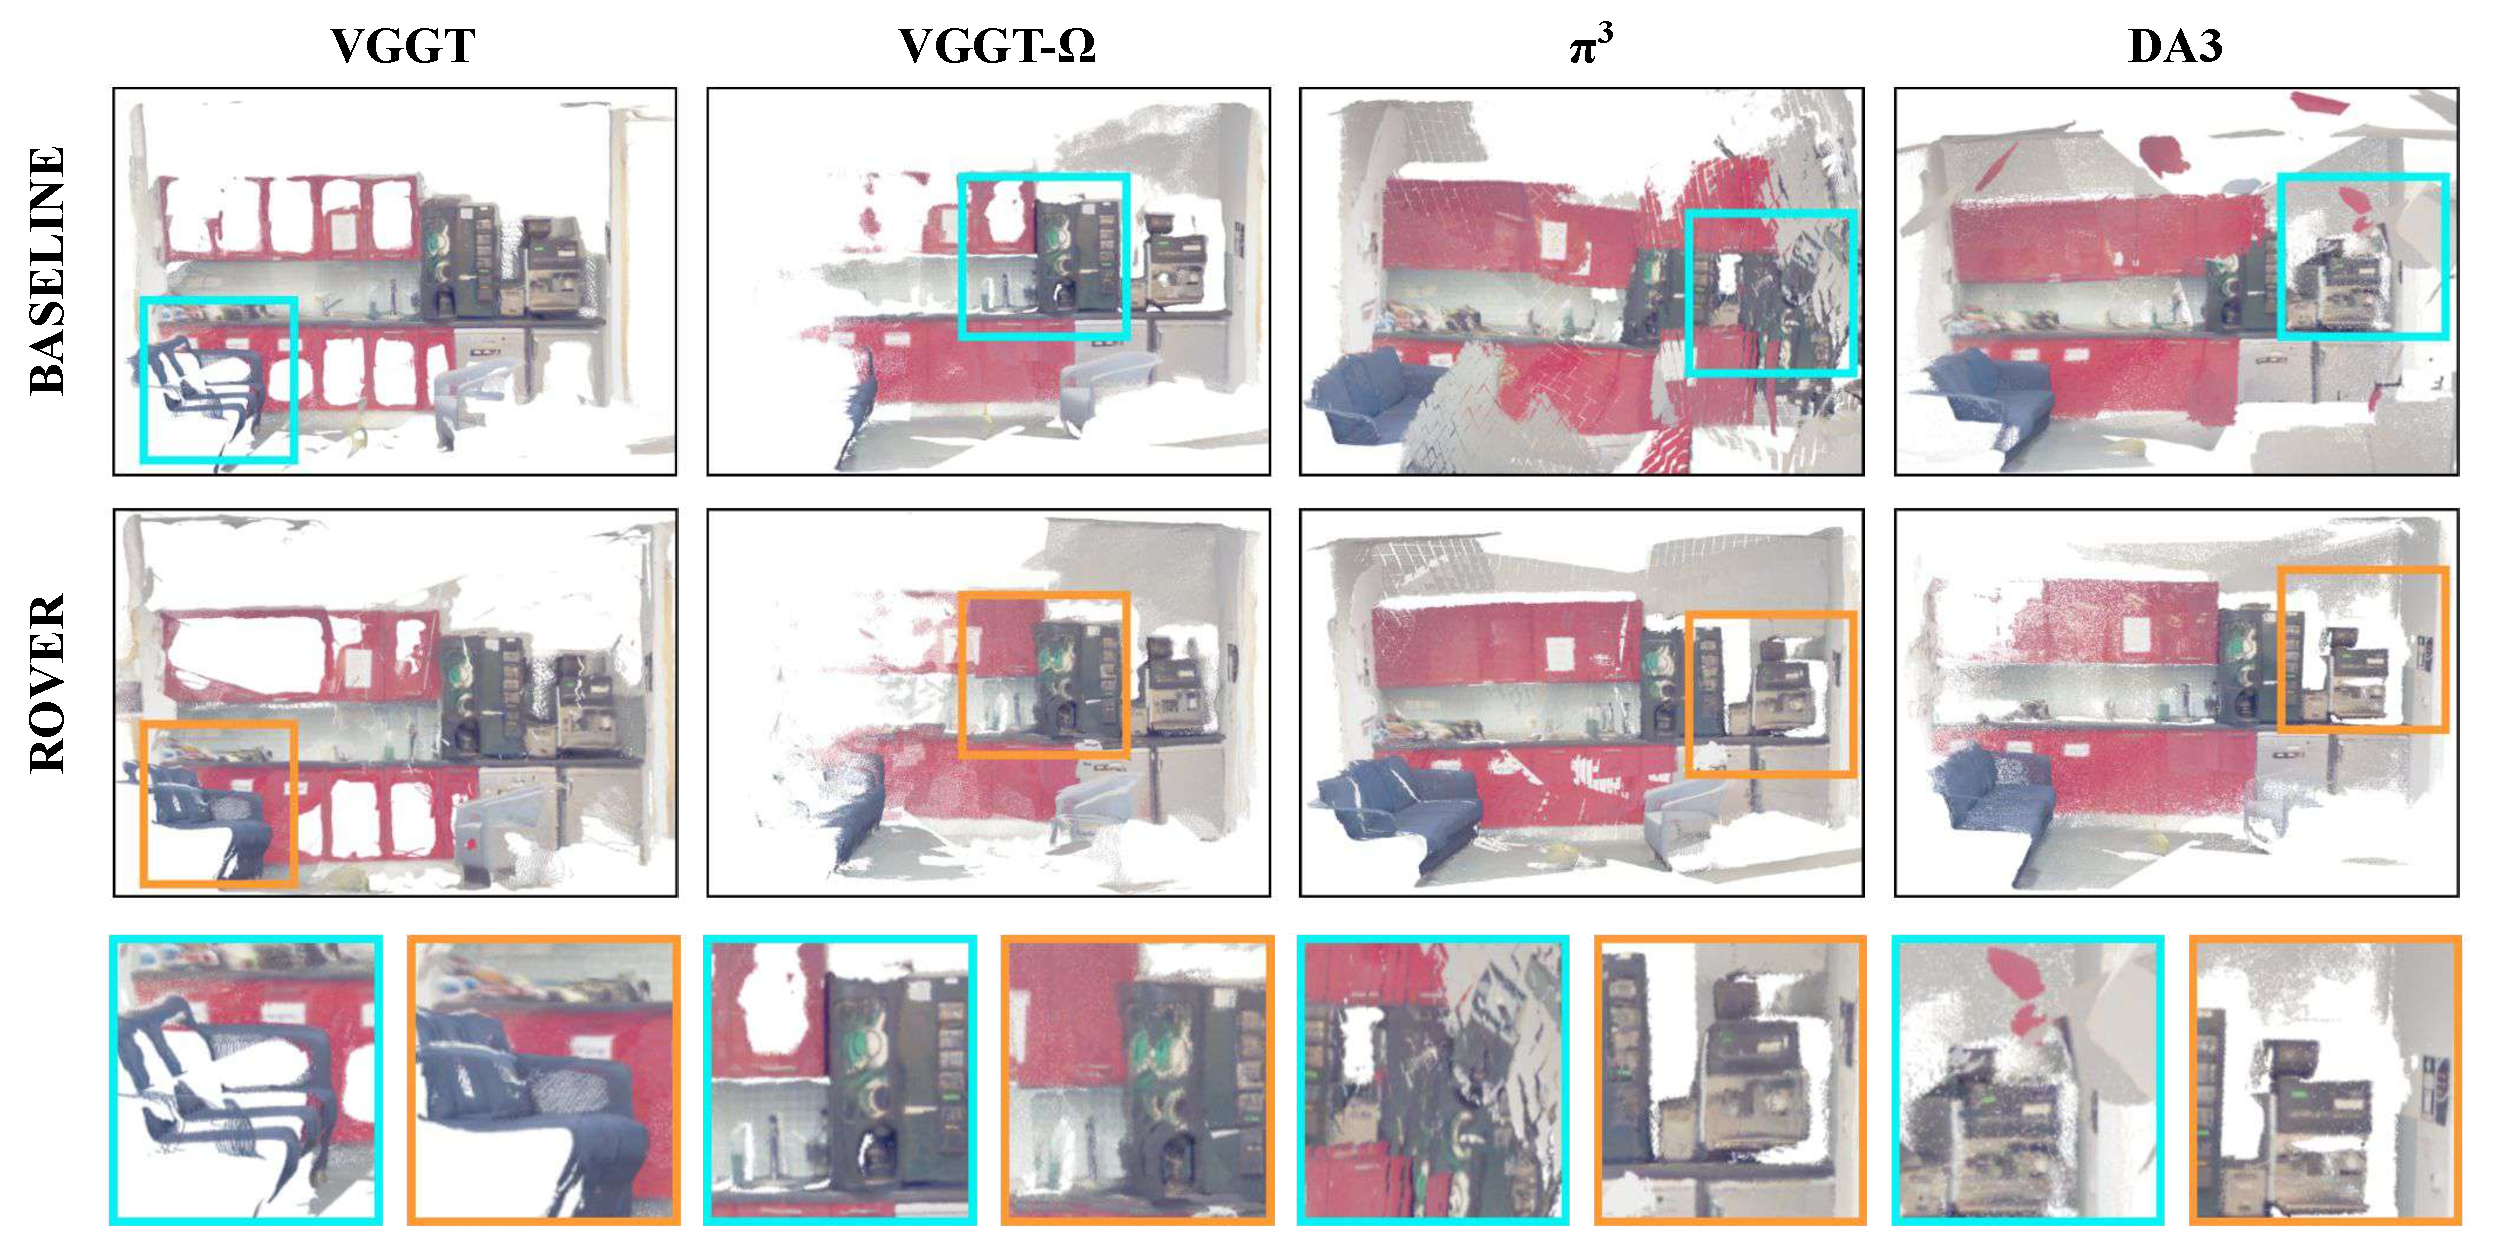
\includegraphics[width=0.97\textwidth]{supplementary_figures/pointcloud_comparisons/supplementary_fig_2.2.pdf}
\caption{\textbf{Qualitative comparison on the 7-Scenes dataset (Red Kitchen scene)}. Close-up comparisons showing geometric alignment and wall boundary recovery under ROVER.}
\label{fig:pc_7scenes_kitchen}

\end{figure*}
%%%%%%%%%%%%%%%%%%%%%%%%%%%%%%%%%%%%%%%%%%%%%%%

% \begin{figure*}[h]
% \centering
% 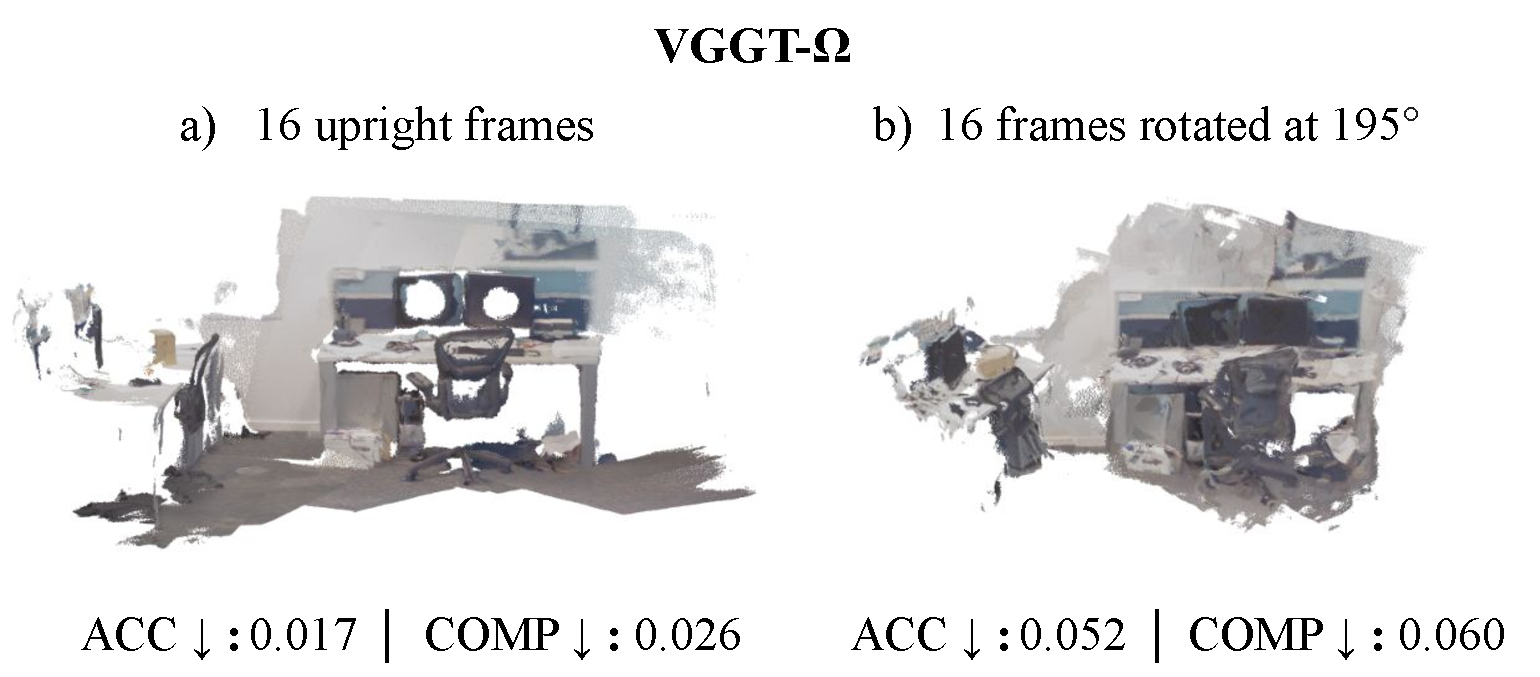
\includegraphics[width=0.86\textwidth]{Figures/pc_comparison.pdf}
% \caption{\textbf{Comparison between upright inputs (left) and inputs rotated by 195$^\circ$ (right).} The reconstructed point cloud degrades even when the same rotation is applied consistently to all input images.}
% \label{fig:all_rot}
% \end{figure*}


\begin{figure}[H]
\centering
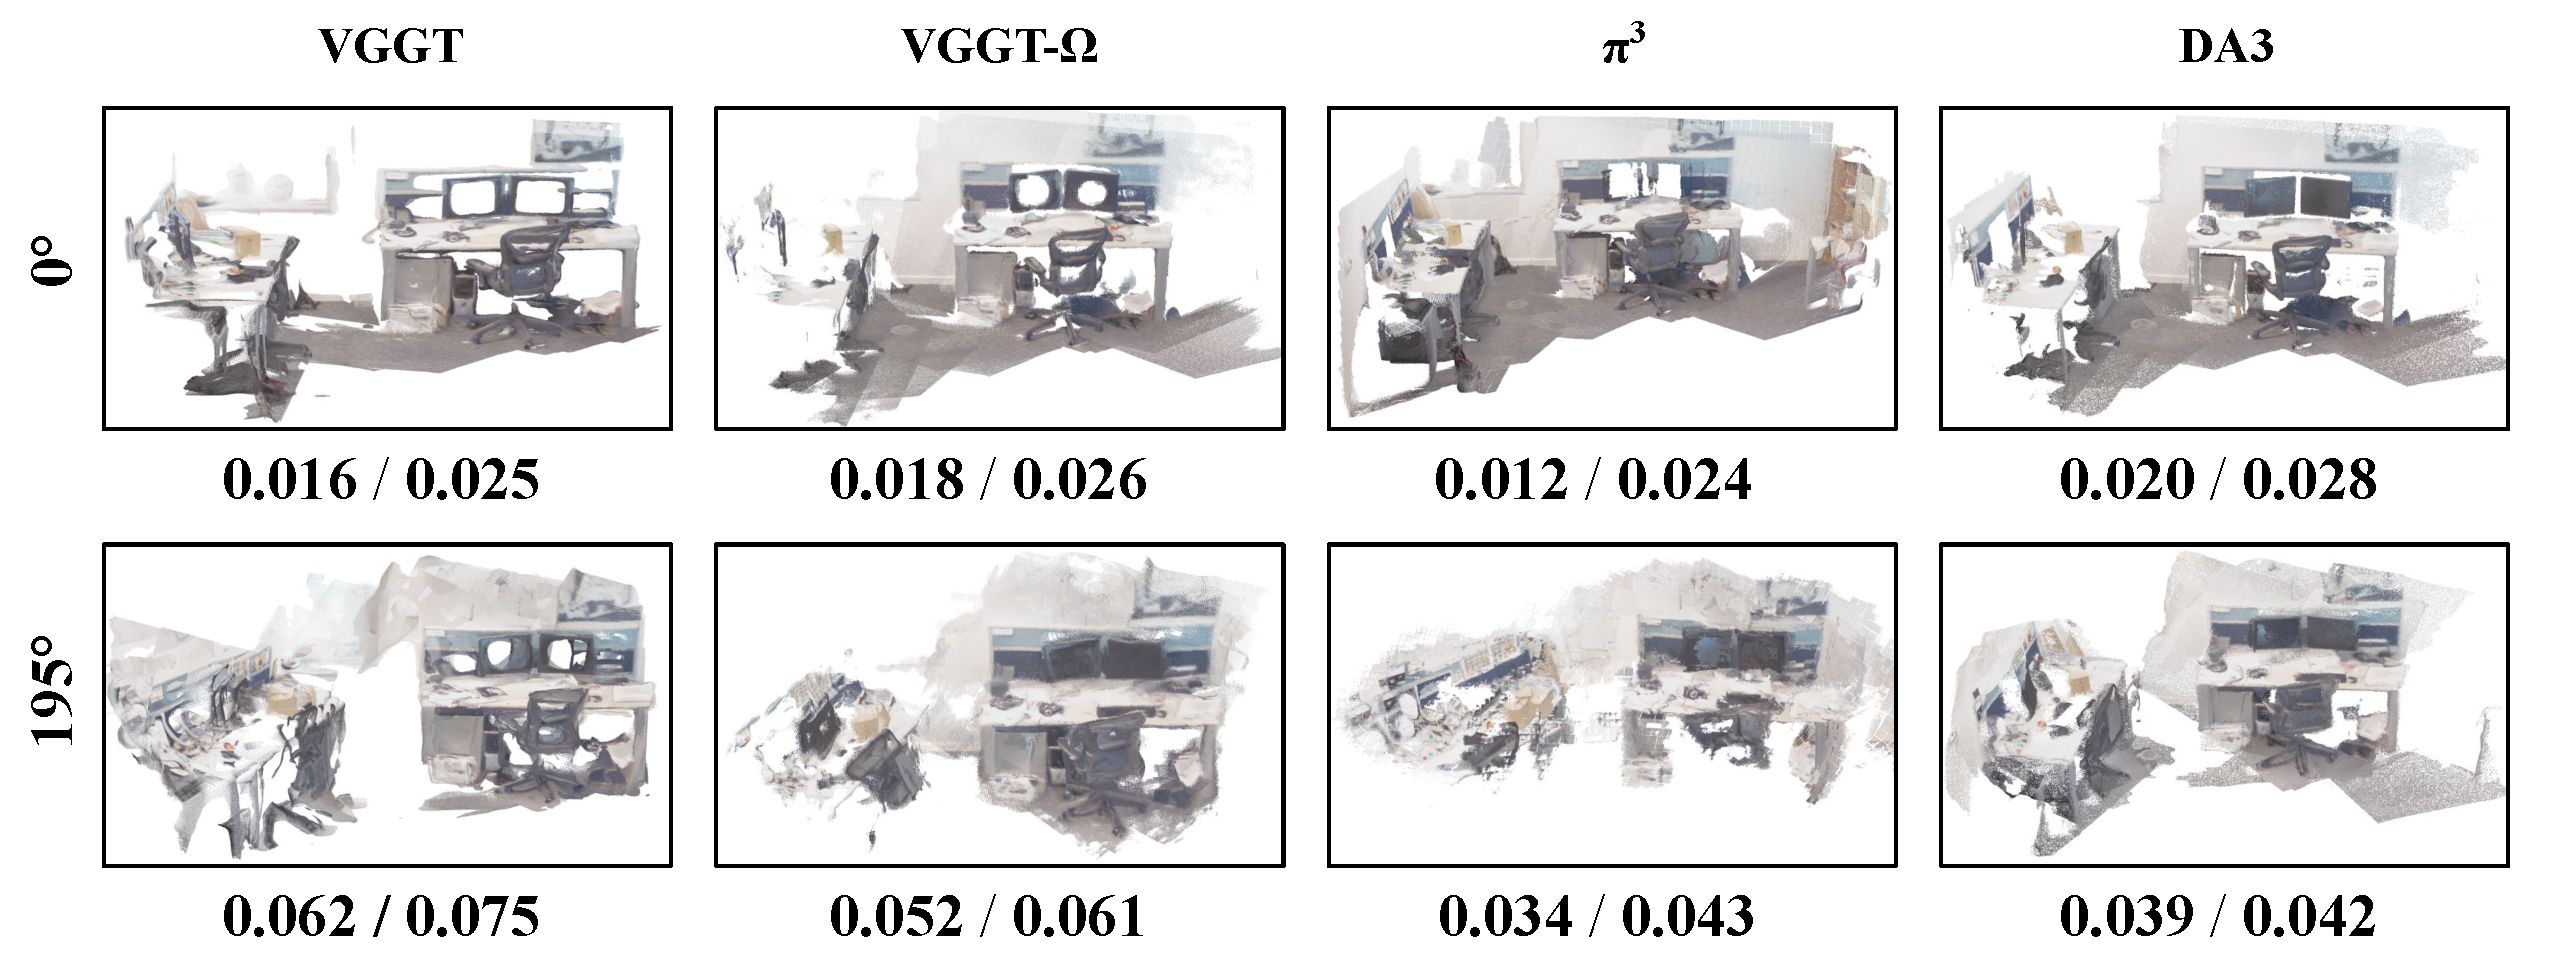
\includegraphics[width=\linewidth]{supplementary_figures/rotation_pc_comparison.pdf}
\caption{\textbf{Degradation under uniform roll on ETH3D (\emph{office}).} Point cloud reconstructions comparing clean upright views ($0^\circ$, top row) with sequences where every input view is rotated identically by $195^\circ$ (bottom row). Numbers denote Accuracy (Acc $\downarrow$) / Completeness (Comp $\downarrow$) in meters relative to ground truth . Degradation occurs despite identical relative poses between views, confirming reliance on an absolute upright prior.}
\label{fig:uniform_rotation_office}
\end{figure}

\section{Sensitivity to Yaw Rotations}
\label{sec:pose_yaw}
We additionally evaluate sensitivity to camera rotations about the yaw axis on NRGB-D, 7-Scenes, and Tanks\&Temples in~\Cref{tab:yaw_metrics}. Following the evaluation protocol described in~\Cref{sec:experimental_setup}, we evaluate the four non-zero rotation levels, with selected views independently assigned yaw perturbations from $[-20^\circ,+20^\circ]$. Large perturbation across yaw will lead to change in viewpoint of the scene which is not a manisfestation of UprightBias thus we restrict the evaluation to limited perturbation.  The corresponding camera poses are perturbed and new views are rendered using~\Cref{sec:rendering_based_rotation}. Overall, yaw perturbations introduce moderate degradation, particularly on Tanks\&Temples. For example, $\pi^3$ decreases from $0.721$ to $0.667$ N.C., while MapAnything decreases from $0.627$ to $0.592$ N.C. and from $94.53$ to $92.57$ AUC$_{30}$. 
\begin{table}[h]
\centering
\caption{Point-map (N.C., $\uparrow$) and pose (AUC$_{30}$, $\uparrow$) accuracy for upright inputs and inputs rotated about the yaw axis, on NRGBD, 7-Scenes, and Tanks\&Temples.}
\label{tab:yaw_metrics}
\small
\setlength{\tabcolsep}{3.5pt}
\resizebox{\linewidth}{!}{%
\begin{tabular}{l *{3}{cccc}}
\toprule
 & \multicolumn{4}{c}{\textbf{NRGBD}}
 & \multicolumn{4}{c}{\textbf{7-Scenes}}
 & \multicolumn{4}{c}{\textbf{Tanks\&Temples}} \\
\cmidrule(lr){2-5} \cmidrule(lr){6-9} \cmidrule(lr){10-13}

 & \multicolumn{2}{c}{N.C. $\uparrow$}
 & \multicolumn{2}{c}{AUC$_{30}$ $\uparrow$}
 & \multicolumn{2}{c}{N.C. $\uparrow$}
 & \multicolumn{2}{c}{AUC$_{30}$ $\uparrow$}
 & \multicolumn{2}{c}{N.C. $\uparrow$}
 & \multicolumn{2}{c}{AUC$_{30}$ $\uparrow$} \\
\cmidrule(lr){2-3} \cmidrule(lr){4-5}
\cmidrule(lr){6-7} \cmidrule(lr){8-9}
\cmidrule(lr){10-11} \cmidrule(lr){12-13}

\textbf{Method}
& Upright & Rotated & Upright & Rotated
& Upright & Rotated & Upright & Rotated
& Upright & Rotated & Upright & Rotated \\
\midrule

VGGT
& \dd{0.795}{0.030} & \dd{0.788}{0.010}
& \dd{98.65}{0.86} & \dd{97.59}{0.82}
& \dd{0.659}{0.033} & \dd{0.665}{0.006}
& \dd{85.80}{9.53} & \dd{84.44}{2.25}
& \dd{0.685}{0.042} & \dd{0.659}{0.032}
& \dd{94.18}{9.62} & \dd{93.33}{1.63} \\
\addlinespace[3pt]

VGGT-$\Omega$
& \dd{0.825}{0.048} & \dd{0.825}{0.008}
& \dd{99.10}{0.72} & \dd{98.46}{0.63}
& \dd{0.672}{0.040} & \dd{0.679}{0.006}
& \dd{89.35}{5.07} & \dd{87.78}{1.58}
& \dd{0.669}{0.080} & \dd{0.657}{0.023}
& \dd{93.27}{13.12} & \dd{93.52}{0.99} \\
\addlinespace[3pt]

$\pi^3$
& \dd{0.817}{0.066} & \dd{0.808}{0.011}
& \dd{96.17}{2.97} & \dd{95.42}{0.82}
& \dd{0.674}{0.041} & \dd{0.685}{0.008}
& \dd{87.54}{6.31} & \dd{85.94}{1.74}
& \dd{0.721}{0.059} & \dd{0.667}{0.040}
& \dd{97.76}{0.63} & \dd{97.17}{1.30} \\
\addlinespace[3pt]

MapA.
& \dd{0.739}{0.057} & \dd{0.716}{0.017}
& \dd{93.11}{5.13} & \dd{91.59}{1.54}
& \dd{0.623}{0.046} & \dd{0.636}{0.013}
& \dd{76.26}{12.07} & \dd{73.28}{3.17}
& \dd{0.627}{0.052} & \dd{0.592}{0.033}
& \dd{94.53}{0.98} & \dd{92.57}{1.79} \\
\addlinespace[3pt]

DA3
& \dd{0.819}{0.037} & \dd{0.808}{0.014}
& \dd{99.75}{0.38} & \dd{99.53}{0.25}
& \dd{0.676}{0.032} & \dd{0.684}{0.007}
& \dd{88.10}{7.73} & \dd{88.55}{1.48}
& \dd{0.674}{0.051} & \dd{0.661}{0.030}
& \dd{98.58}{2.11} & \dd{98.74}{1.36} \\

\bottomrule
\end{tabular}%
}
\end{table}

\section{The RotMV Dataset}
  \label{sec:rotmv_dataset}
  
  As discussed in \cref{sec:method}, existing multi-view datasets consist predominantly of clean, upright images. Consequently, evaluations on these datasets are
  performed by introducing synthetic camera roll using the controlled rotation synthesis described in \cref{sec:rendering_based_rotation}
  (\cref{alg:rotation_generation}). We present a novel benchmark consisting of seven real-world scenes (\textit{chairs}, \textit{foosball-table}, \textit{building},
  \textit{rooftop}, \textit{room}, \textit{statue}, and \textit{table-tennis}). We capture each scene using a camera ($4.84\,\text{mm}$, $f/1.8$, $12\,\text{MP}$,
  $4096\times3072$ resolution). Each scene is imaged from $16$ fixed viewpoints, and at each viewpoint, the camera is rolled in-plane through $12$ orientations
  spanning a full $360^\circ$ (in $30^\circ$ increments), resulting in $192$ images per scene.
 
  For each viewpoint, we estimate the base camera pose from the upright ($0^\circ$) image using VGGT~\citep{wang2025vggt}. The poses corresponding to the remaining $11$
  roll angles are then derived from this base pose by applying the corresponding in-plane rotation to the camera orientation, while keeping the camera center and viewing
  direction unchanged. Thus, pose estimation is performed only for the upright image at each viewpoint, and the poses for the other roll angles are constructed
  analytically. This enables a robust evaluation of each method under realistic in-plane camera roll, while keeping the underlying scene geometry and viewpoint fixed.

  We show example images from our dataset in Figures \Cref{fig:grid_foosball} and \Cref{fig:grids_chairs_rooftop}.


% =========================================================================
% PAGE 1: Foosball Table (Bottom of Page G-5)
% =========================================================================
\begin{figure}[!htb]
\centering
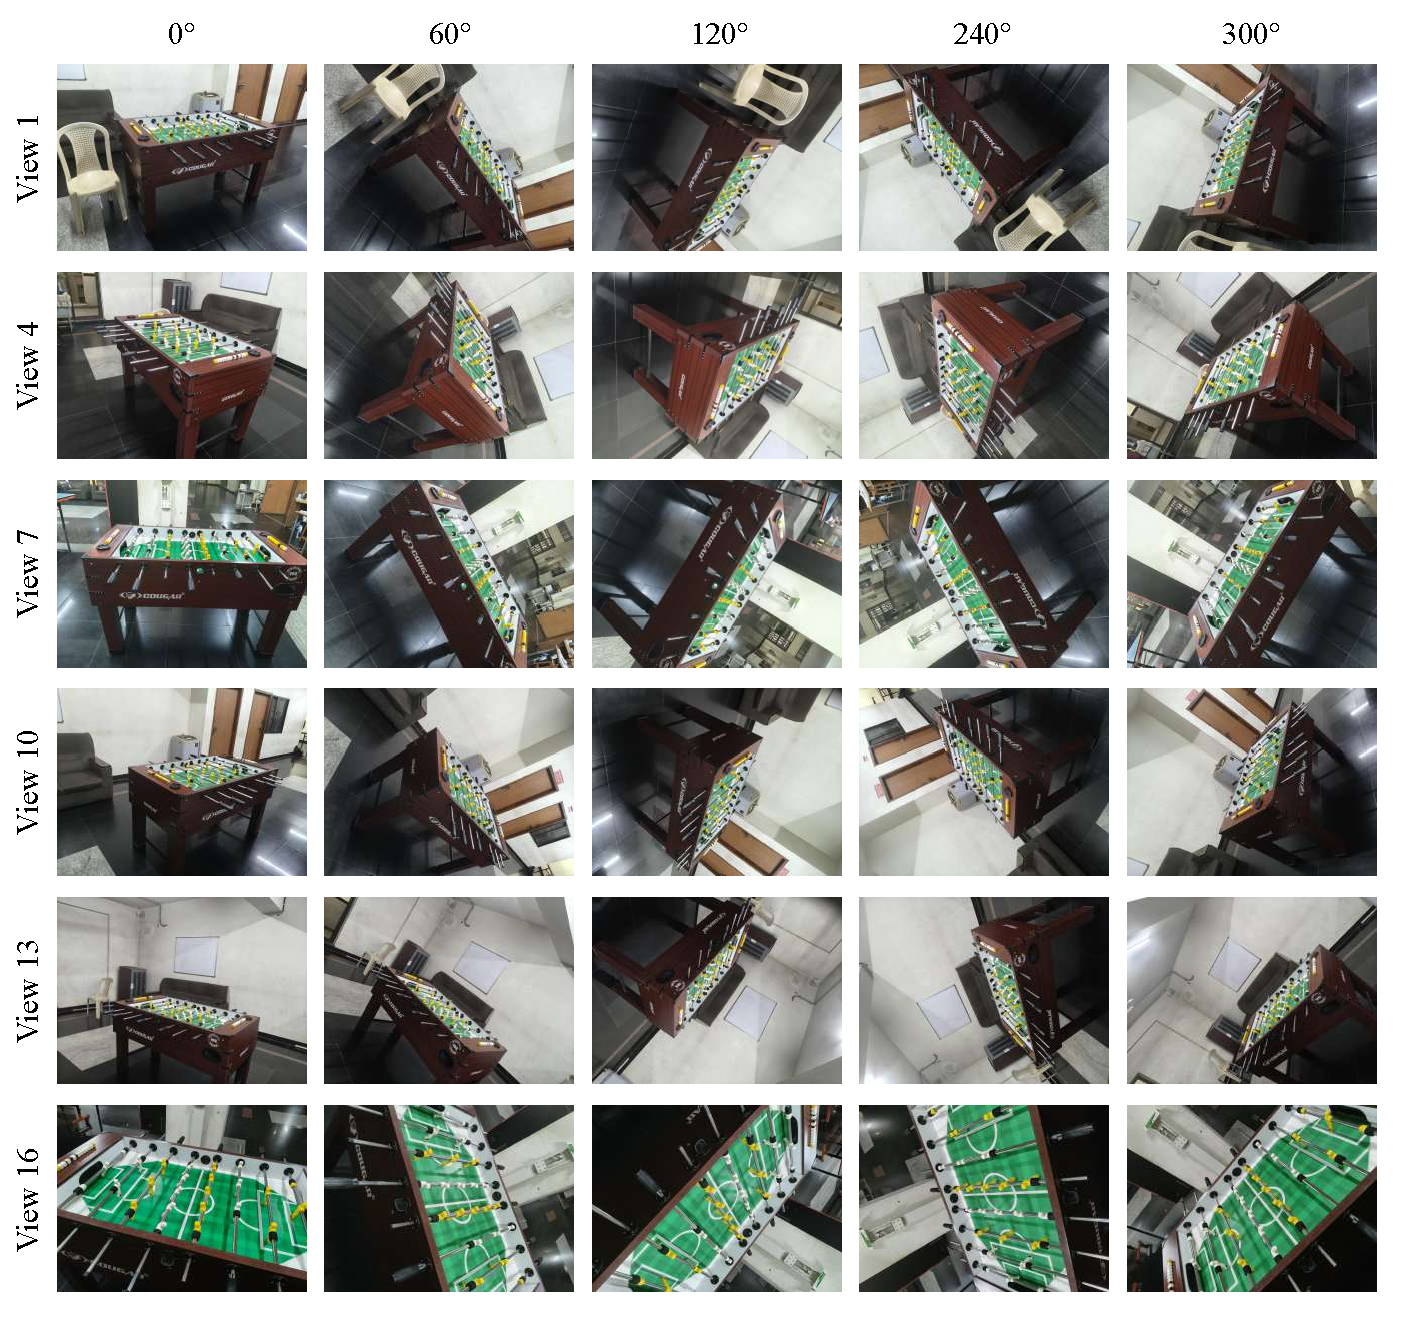
\includegraphics[
    height=0.55\textheight,
    keepaspectratio
]{Figures/captured_supplementary/foosball_compressed.pdf}
\vspace{1mm}
\caption{\textbf{RotMV dataset roll sweeps: Foosball Table (Indoor).}
Sampled views (rows) across in-plane roll angles
($\theta \in [0^\circ, 300^\circ]$, columns).}
\label{fig:grid_foosball}
\end{figure}

% \clearpage

% =========================================================================
% PAGE 2: Chairs & Rooftop
% =========================================================================
\begin{figure}[tbp]
\centering
\vspace*{-6mm}

\begin{subfigure}[tbp]{\textwidth}
    \centering
    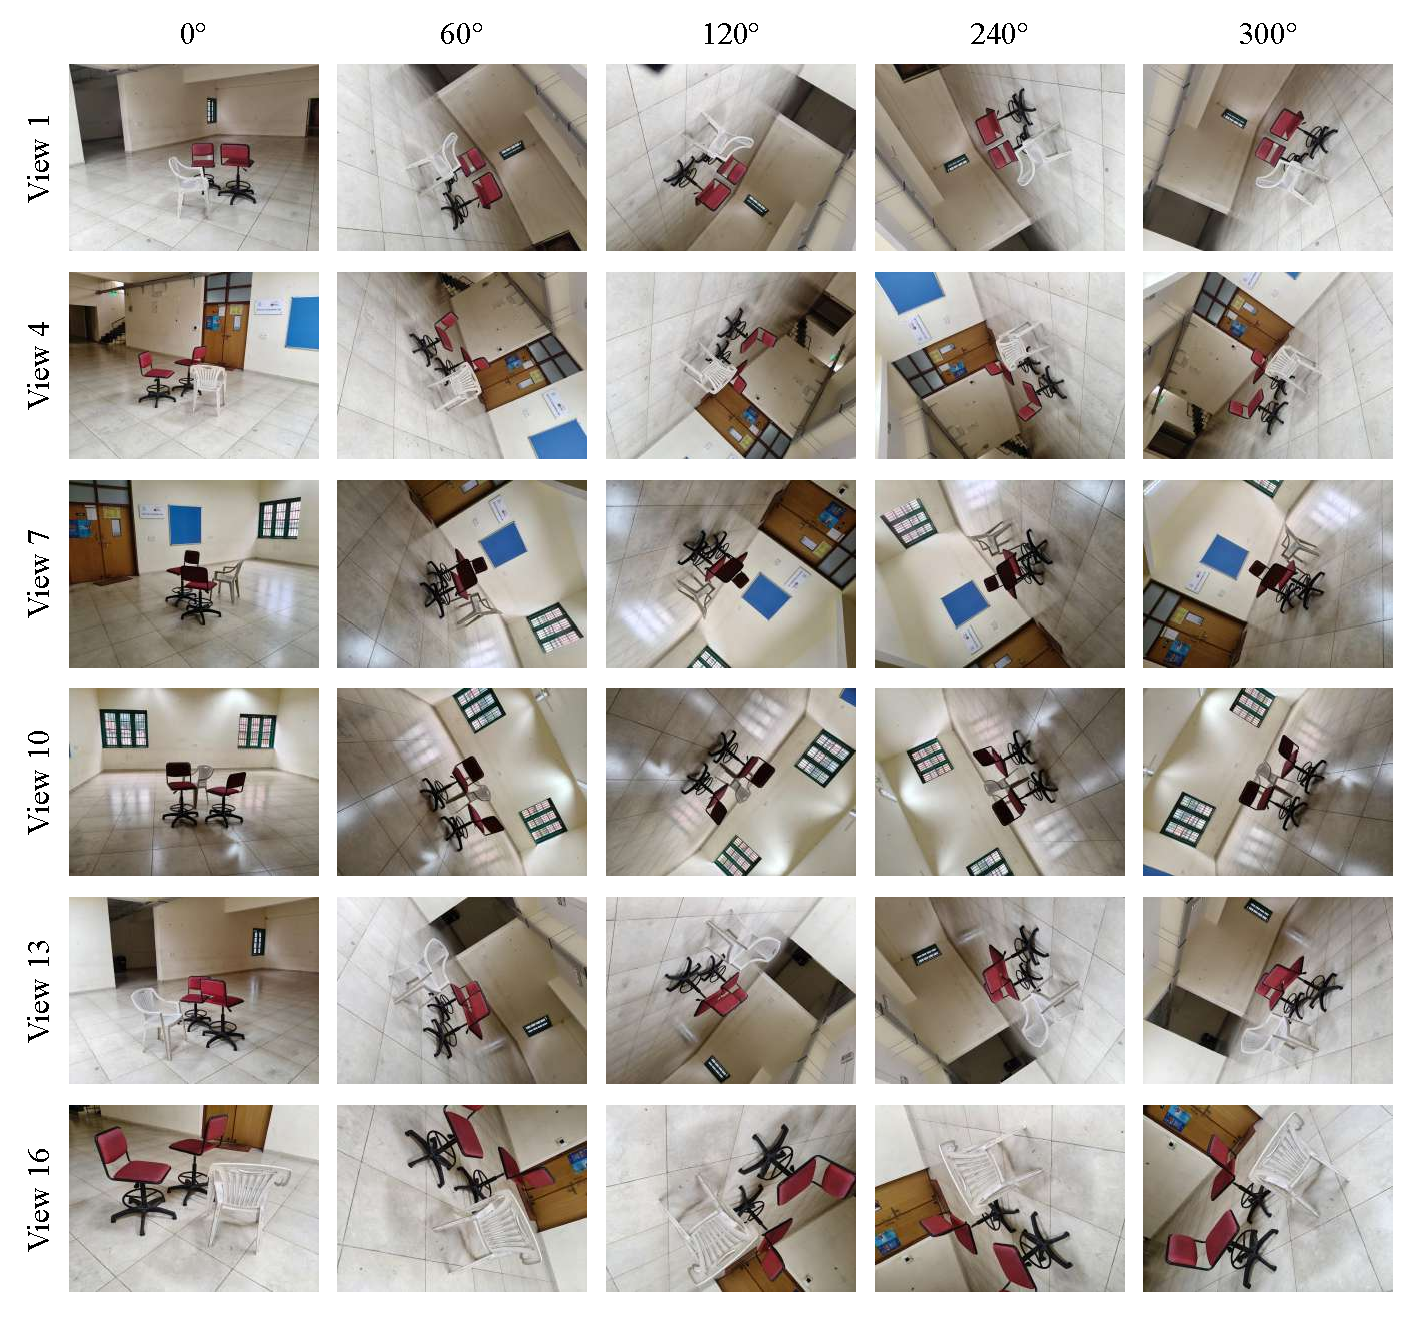
\includegraphics[
        height=0.45\textheight,
        keepaspectratio
    ]{Figures/captured_supplementary/chairs_compressed.pdf}
    \caption{Chairs (Indoor)}
    \label{fig:grid_chairs}
\end{subfigure}

\vspace{2mm}

\begin{subfigure}[tbp]{\textwidth}
    \centering
    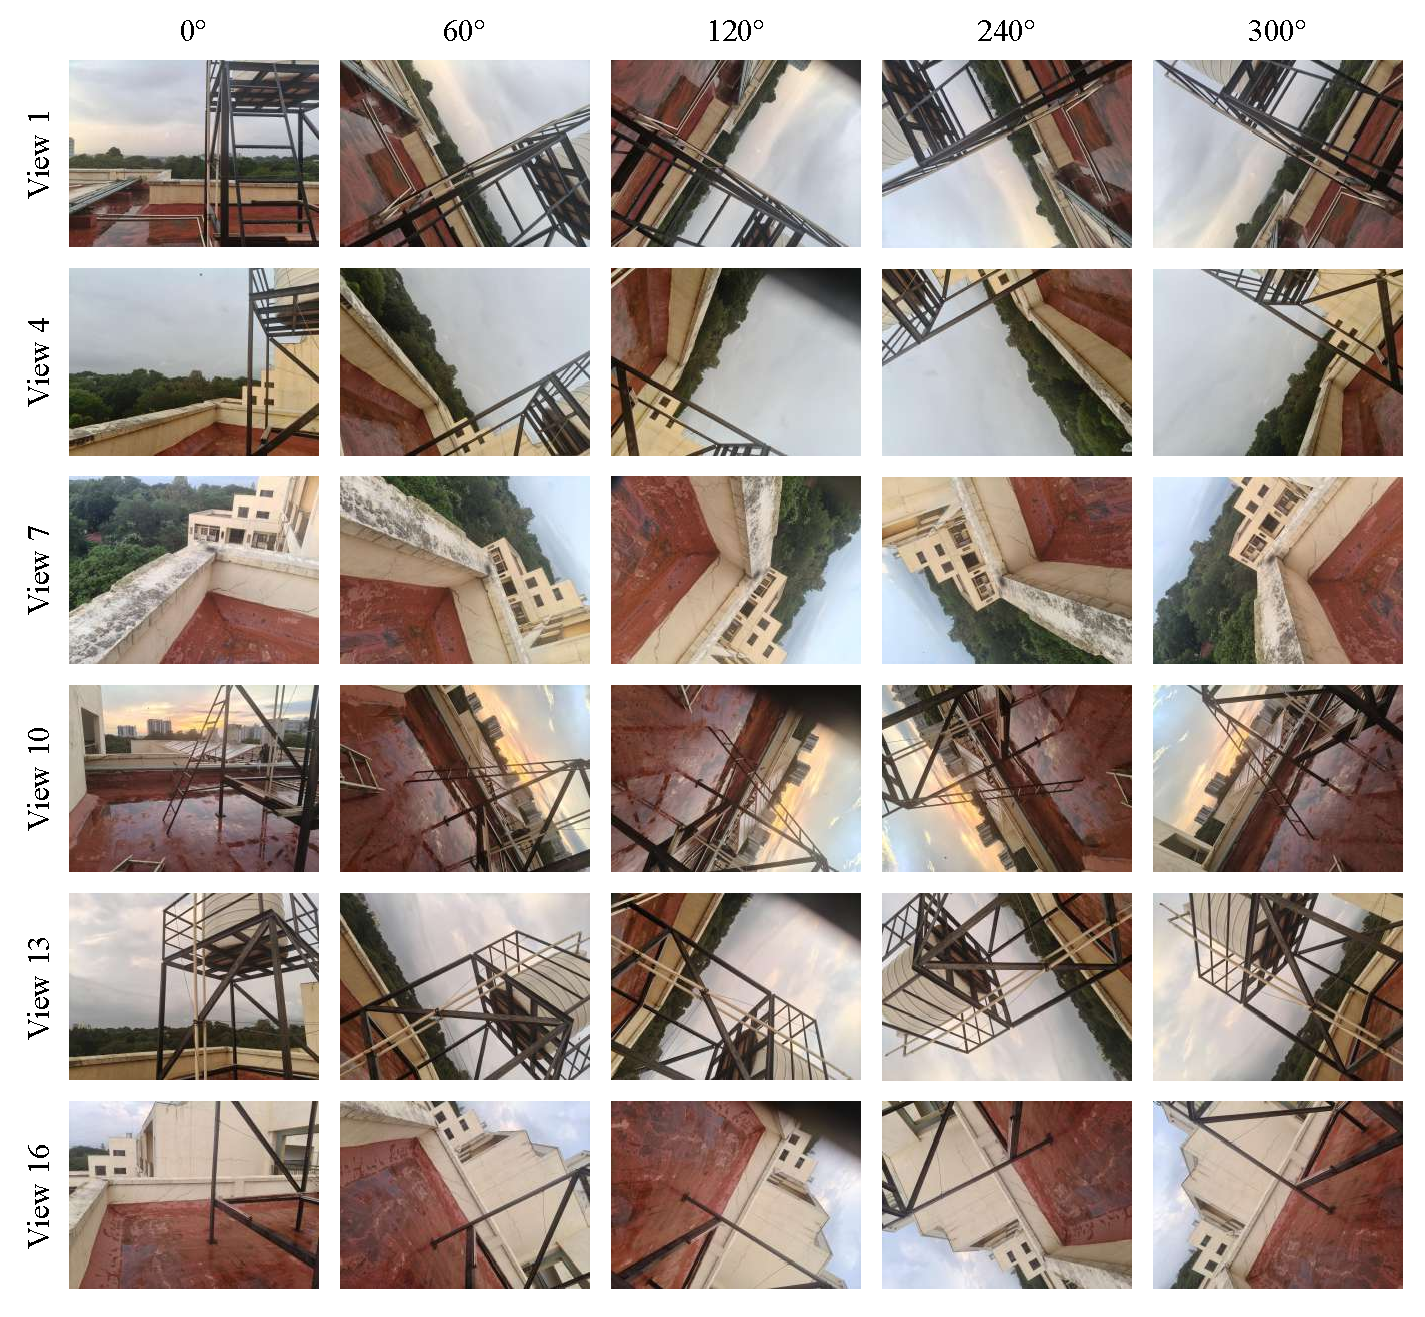
\includegraphics[
        height=0.45\textheight,
        keepaspectratio
    ]{Figures/captured_supplementary/rooftop_compressed.pdf}
    \caption{Rooftop (Outdoor)}
    \label{fig:grid_rooftop}
\end{subfigure}

\vspace{1mm}
\caption{\textbf{RotMV dataset roll sweeps: Chairs and Rooftop.}
Sampled views (rows) across in-plane roll angles
($\theta \in [0^\circ, 300^\circ]$, columns).}
\label{fig:grids_chairs_rooftop}
\end{figure}

% \clearpage
% \clearpage
% % =========================================================================
% % PAGE 1: Indoor Scenes (Foosball Table & Chairs)
% % =========================================================================
% \begin{figure*}[p]
% \centering
% \vspace*{-6mm} % Offsets float centering to utilize top margin

% % --- Top Grid: Foosball Table ---
% \begin{subfigure}[b]{\textwidth}
%   \centering
%   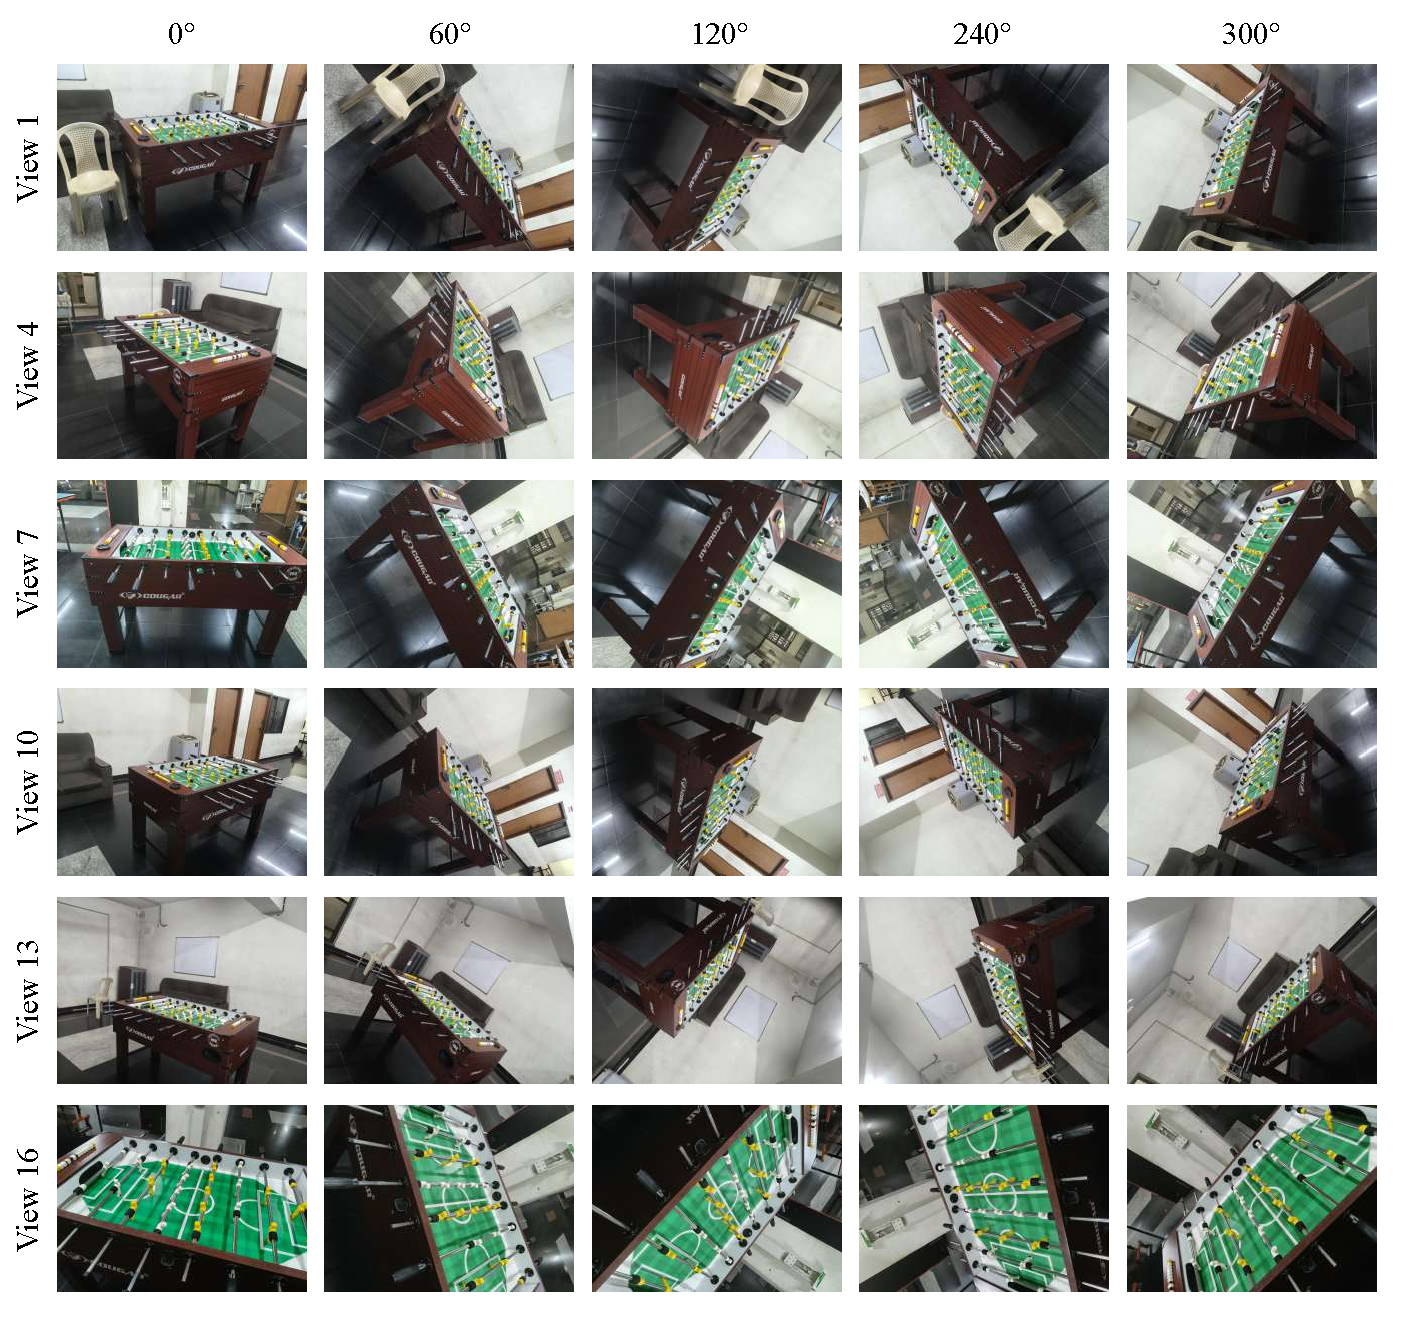
\includegraphics[height=0.47\textheight,keepaspectratio]{Figures/captured_supplementary/foosball_compressed.pdf}
%   \caption{Foosball Table}
%   \label{fig:grid_foosball}
% \end{subfigure}

% \vspace{2mm}

% % --- Bottom Grid: Chairs ---
% \begin{subfigure}[b]{\textwidth}
%   \centering
%   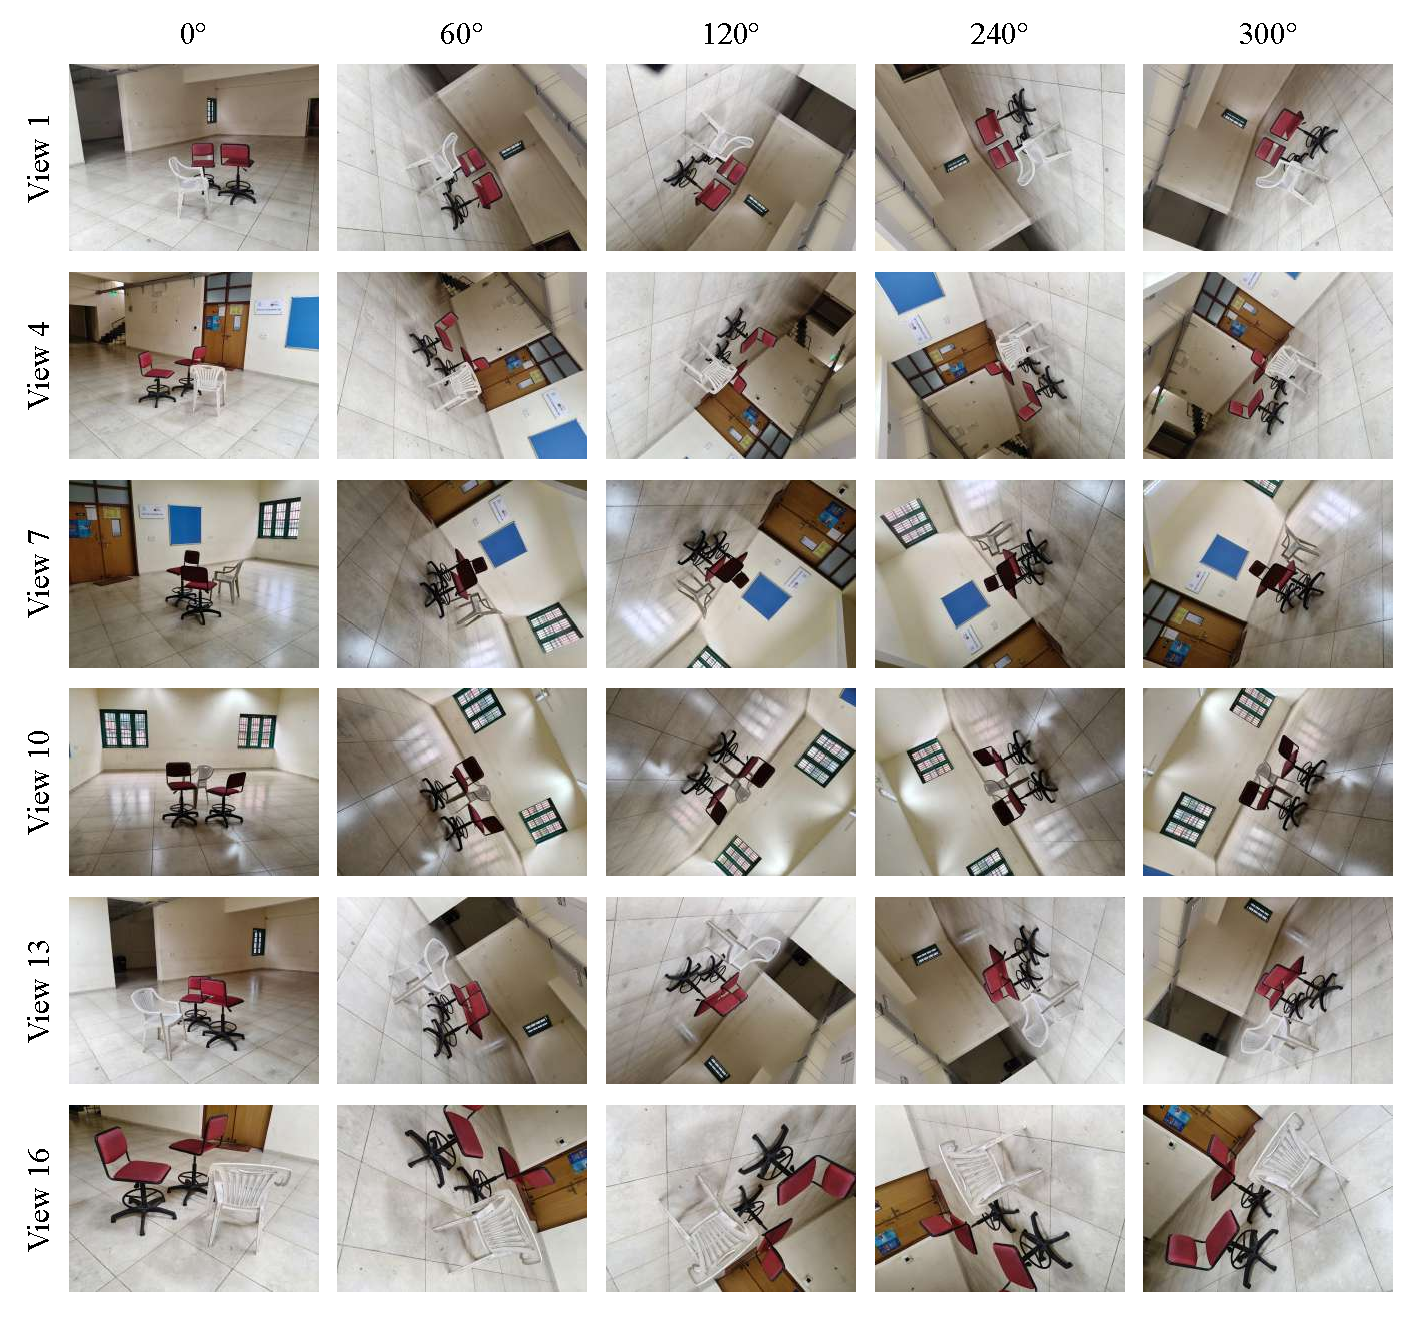
\includegraphics[height=0.48\textheight,keepaspectratio]{Figures/captured_supplementary/chairs_compressed.pdf}
%   \caption{Chairs}
%   \label{fig:grid_chairs}
% \end{subfigure}

% \vspace{1mm}
% \caption{\textbf{ROTMV dataset roll sweeps (Indoor).} Sampled views (rows) across in-plane roll angles ($0^\circ$- $300^\circ$, columns).}
% \label{fig:grids_indoor}
% \end{figure*}


% \clearpage
% % =========================================================================
% % PAGE 2: Outdoor Scenes (Building & Rooftop)
% % =========================================================================
% \begin{figure*}[p]
% \centering
% \vspace*{-6mm} % Offsets float centering to utilize top margin

% % --- Top Grid: Building ---
% % \begin{subfigure}[b]{\textwidth}
% %   \centering
% %   \includegraphics[height=0.47\textheight,keepaspectratio]{Figures/captured_supplementary/building_compressed.pdf}
% %   \caption{Building}
% %   \label{fig:grid_building}
% % \end{subfigure}

% \vspace{-4mm}

% % --- Bottom Grid: Rooftop ---
% \begin{subfigure}[b]{\textwidth}
%   \centering
%   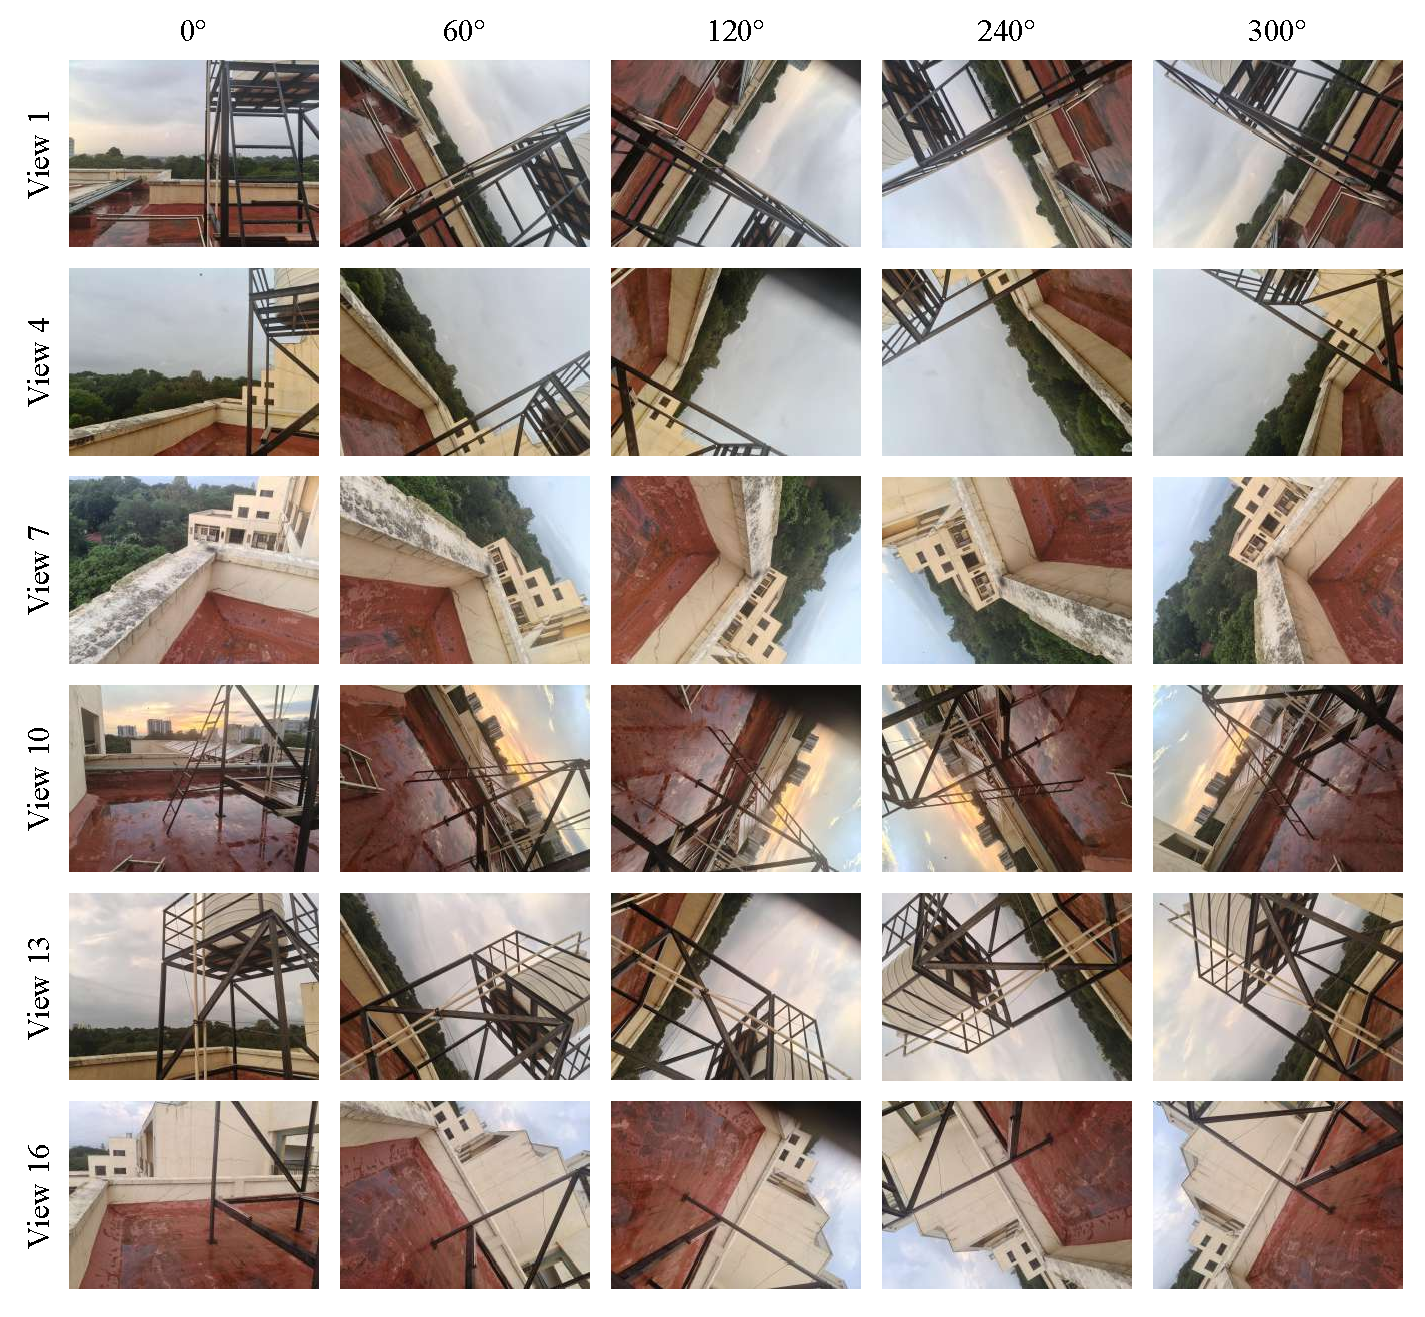
\includegraphics[height=0.47\textheight,keepaspectratio]{Figures/captured_supplementary/rooftop_compressed.pdf}
%   \caption{Rooftop}
%   \label{fig:grid_rooftop}
% \end{subfigure}

% \vspace{1mm}
% \caption{\textbf{ROTMV dataset roll sweeps (Outdoor).} Sampled views (rows) across in-plane roll angles ($0^\circ$- $300^\circ$, columns).}
% \label{fig:grids_outdoor}
% \end{figure*}




\section{Visual Quality Assessment and Rejection Statistics}
\label{sec:image_statistics}
% We render rotated images as described in the algorithm in ~\cref{alg:rotation_generation}. We compare the artifacts produced without and with Difix3D denoising step in ~\Cref{fig:denoise-examples-1} and \Cref{fig:denoise-examples-2}. We observe reconstruction through 3DGS with dense set of images (for ex.: DTU, Mip-NeRF 360) results in good reconstruction, where VisualQuality-R1\citep{wu2026visualquality} outputs a score of $\geq 4.0$ on a scale of $[0-5]$. Therefore, we run Difix3D Denoising only for images generated from the other sparse datasets. After this step, we filter images with artifacts using VisualQuality-R1 pipeline where we pass the rotated image and it's 0° counterpart along with a prompt to provide a quality score in the range $[0-5]$. Thereafter, we manually filter the images to filter out reconstruction with obvious artifacts. We provide the statistics for the generated and filtered images in ~\cref{tab:img_stats}. Additionally, we provide example images from the quality filtering pipeline in ~\cref{fig:quality-filtering}

  We render rotated images as described in \cref{alg:rotation_generation}. To reduce rendering artifacts, we use only the single-step diffusion denoiser (Difix)
  from Difix3D+~\citep{wu2025difix3d}, applied independently to each rendered view as a post-processing step. We compare renders without and with
  this denoising step in \Cref{fig:denoise-examples-1} and \ref{fig:denoise-examples-2}. We observe that 3DGS reconstructions from dense image sets (e.g., DTU and
  Mip-NeRF 360) already yield high-quality renders, for which VisualQuality-R1~\citep{wu2026visualquality} outputs a score of $\geq 4.0$ on a scale of $[0, 5]$.
  Therefore, we apply the Difix denoiser only to images rendered from the remaining, sparser datasets. We then filter images with artifacts using VisualQuality-R1,
  passing each rotated image together with its $0^\circ$ counterpart and a prompt asking for a quality score in the range $[0, 5]$. Finally, we manually remove any
  remaining renders with obvious artifacts. Statistics for the generated and filtered images are given in \cref{tab:img_stats}, and example images from the quality
  filtering pipeline are shown in \cref{fig:quality-filtering}.

  
\begin{table}[tbp]
\centering
\small
\caption{Statistics of VLM (VisualQuality-R1) based and manual rejection during dataset curation using controlled rotation synthesis.}
\label{tab:img_stats}

\resizebox{0.9\linewidth}{!}{%
% \begin{tabular}{lccccc}
% \toprule
% Dataset & Initial images & Rejected by VQ-R1 & Manually reviewed & Manually rejected & Final \\
% \midrule
% Tanks\&Temples & 1{,}802 & 1{,}552 & 250 & 45 & 205 \\
% 7-Scenes       & 4{,}300 & 3{,}950 & 350 & 28 & 322 \\
% NRGBD          & 1{,}101 & 661   & 440 & 67 & 373 \\
% \bottomrule
% \end{tabular}%
% }
\begin{tabular}{lcccc}
\toprule
Dataset & Initial images & Rejected by VQ-R1 & Manually rejected & Final \\
\midrule
Tanks\&Temples & 43{,}248 & 37{,}248 & 1{,}080 & 4{,}920 \\
% 7\text{-}Scenes & 103{,}200 & 94{,}800 & 672 & 7{,}728 \\
NRGBD & 26{,}424 & 15{,}864 & 1{,}608 & 8{,}952 \\
ETH3D          & 10{,}896 & 9550    & 534 & 812 \\
% ETH3d after removing office dataset
\bottomrule
\end{tabular}%
}


\end{table}

% Make figure captions use the same size as the figure labels.
\captionsetup[figure]{font=small}

% ============================================================
% Denoising qualitative examples — page 1
% ============================================================

\begin{figure}[h]
\centering
\small

% \begin{tabular}{ccc}
% \textbf{Reference} &
% \textbf{Rotated (pre-denoise)} &
% \textbf{Denoised (ours)} \\[4pt]

% \includegraphics[width=0.30\linewidth]
% {supplementary_figures/difix3d_pics/eth3d_courtyard_345_0_ref.jpg} &
% \includegraphics[width=0.30\linewidth]
% {supplementary_figures/difix3d_pics/eth3d_courtyard_345_0_raw.jpg} &
% \includegraphics[width=0.30\linewidth]
% {supplementary_figures/difix3d_pics/eth3d_courtyard_345_0_denoised.jpg} \\

% \multicolumn{3}{c}
% {eth3d / courtyard / 345$^\circ$, score 4.25} \\[4pt]


% \includegraphics[width=0.30\linewidth]
% {supplementary_figures/difix3d_pics/eth3d_pipes_345_1_ref.jpg} &
% \includegraphics[width=0.30\linewidth]
% {supplementary_figures/difix3d_pics/eth3d_pipes_345_1_raw.jpg} &
% \includegraphics[width=0.30\linewidth]
% {supplementary_figures/difix3d_pics/eth3d_pipes_345_1_denoised.jpg} \\

% \multicolumn{3}{c}
% {eth3d / pipes / 345$^\circ$, score 4.25} \\[4pt]


% \includegraphics[width=0.30\linewidth]
% {supplementary_figures/difix3d_pics/eth3d_electro_330_2_ref.jpg} &
% \includegraphics[width=0.30\linewidth]
% {supplementary_figures/difix3d_pics/eth3d_electro_330_2_raw.jpg} &
% \includegraphics[width=0.30\linewidth]
% {supplementary_figures/difix3d_pics/eth3d_electro_330_2_denoised.jpg} \\

% \multicolumn{3}{c}
% {eth3d / electro / 330$^\circ$, score 4.20} \\[4pt]


% \includegraphics[width=0.30\linewidth]
% {supplementary_figures/difix3d_pics/eth3d_electro_60_3_ref.jpg} &
% \includegraphics[width=0.30\linewidth]
% {supplementary_figures/difix3d_pics/eth3d_electro_60_3_raw.jpg} &
% \includegraphics[width=0.30\linewidth]
% {supplementary_figures/difix3d_pics/eth3d_electro_60_3_denoised.jpg} \\

% \multicolumn{3}{c}
% {eth3d / electro / 60$^\circ$, score 3.80} \\[4pt]


% \includegraphics[width=0.30\linewidth]
% {supplementary_figures/difix3d_pics/eth3d_pipes_60_4_ref.jpg} &
% \includegraphics[width=0.30\linewidth]
% {supplementary_figures/difix3d_pics/eth3d_pipes_60_4_raw.jpg} &
% \includegraphics[width=0.30\linewidth]
% {supplementary_figures/difix3d_pics/eth3d_pipes_60_4_denoised.jpg} \\

% \multicolumn{3}{c}
% {eth3d / pipes / 60$^\circ$, score 3.80} \\[4pt]

% \end{tabular}
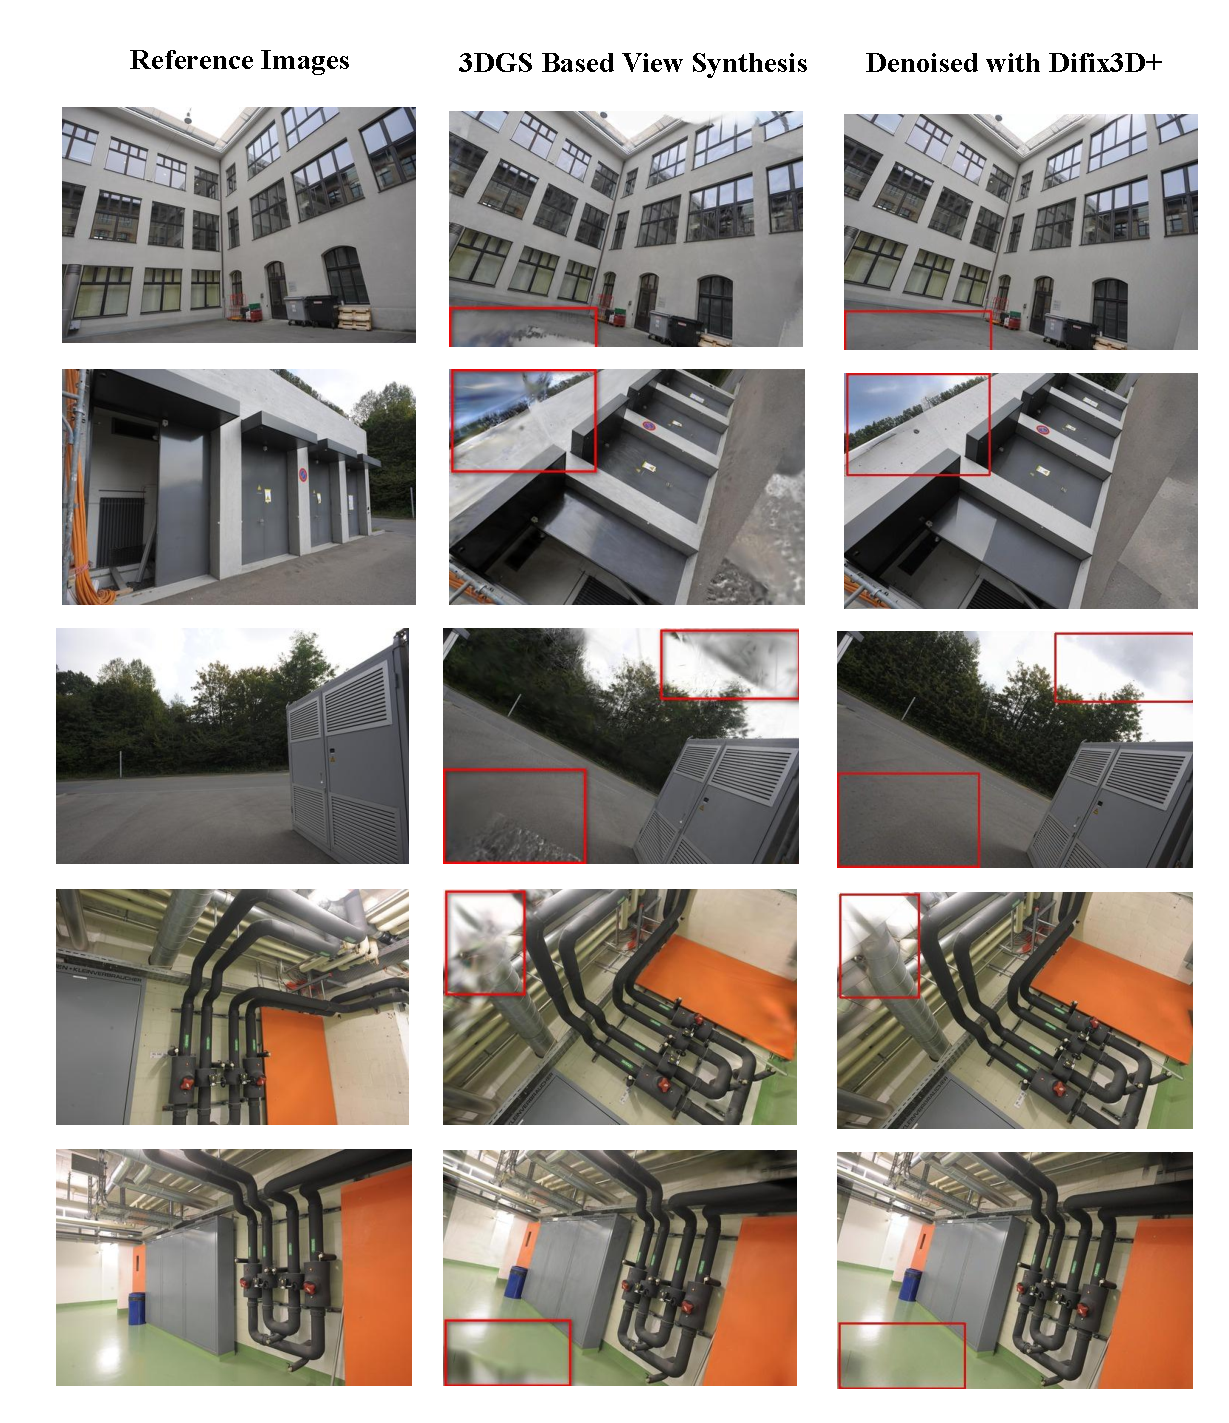
\includegraphics[width=0.98\linewidth,height=0.88\textheight,keepaspectratio]{supplementary_figures/difix3d_examples/difix-1-1.pdf}
\caption{\textbf{Effect of Difix denoising on 3DGS-based rotated view synthesis.} Reference images (left), 3DGS-synthesized views (middle), and their denoised counterparts (right), shown for the \textit{Courtyard}, \textit{Electro} and \textit{Pipes}  scenes from ETH3D. Red boxes mark artifacts in the synthesized views, with corresponding regions in the denoised views to indicate that the artifacts are removed or reduced.}
\label{fig:denoise-examples-1}

\end{figure}


% ============================================================
% Denoising qualitative examples — page 2
% ============================================================

\begin{figure}[h]
% \ContinuedFloat
\centering
\small

% \begin{tabular}{ccc}
% \textbf{Reference} &
% \textbf{Rotated (pre-denoise)} &
% \textbf{Denoised (ours)} \\[4pt]

% \includegraphics[width=0.30\linewidth]
% {supplementary_figures/difix3d_pics/tnt_Meetingroom_roll_15_5_ref.jpg} &
% \includegraphics[width=0.30\linewidth]
% {supplementary_figures/difix3d_pics/tnt_Meetingroom_roll_15_5_raw.jpg} &
% \includegraphics[width=0.30\linewidth]
% {supplementary_figures/difix3d_pics/tnt_Meetingroom_roll_15_5_denoised.jpg} \\

% \multicolumn{3}{c}
% {tnt / Meetingroom / roll 15$^\circ$, score 4.20} \\[4pt]


% \includegraphics[width=0.30\linewidth]
% {supplementary_figures/difix3d_pics/tnt_Meetingroom_roll_15_6_ref.jpg} &
% \includegraphics[width=0.30\linewidth]
% {supplementary_figures/difix3d_pics/tnt_Meetingroom_roll_15_6_raw.jpg} &
% \includegraphics[width=0.30\linewidth]
% {supplementary_figures/difix3d_pics/tnt_Meetingroom_roll_),15_6_denoised.jpg} \\

% \multicolumn{3}{c}
% {tnt / Meetingroom / roll 15$^\circ$, score 4.20} \\[4pt]


% \includegraphics[width=0.30\linewidth]
% {supplementary_figures/difix3d_pics/tnt_Church_roll_15_7_ref.jpg} &
% \includegraphics[width=0.30\linewidth]
% {supplementary_figures/difix3d_pics/tnt_Church_roll_15_7_raw.jpg} &
% \includegraphics[width=0.30\linewidth]
% {supplementary_figures/difix3d_pics/tnt_Church_roll_15_7_denoised.jpg} \\

% \multicolumn{3}{c}
% {tnt / Church / roll 15$^\circ$, score 4.00} \\[4pt]


% \includegraphics[width=0.30\linewidth]
% {supplementary_figures/difix3d_pics/tnt_Church_roll_15_8_ref.jpg} &
% \includegraphics[width=0.30\linewidth]
% {supplementary_figures/difix3d_pics/tnt_Church_roll_15_8_raw.jpg} &
% \includegraphics[width=0.30\linewidth]
% {supplementary_figures/difix3d_pics/tnt_Church_roll_15_8_denoised.jpg} \\

% \multicolumn{3}{c}
% {tnt / Church / roll 15$^\circ$, score 4.00} \\[4pt]

% \end{tabular}
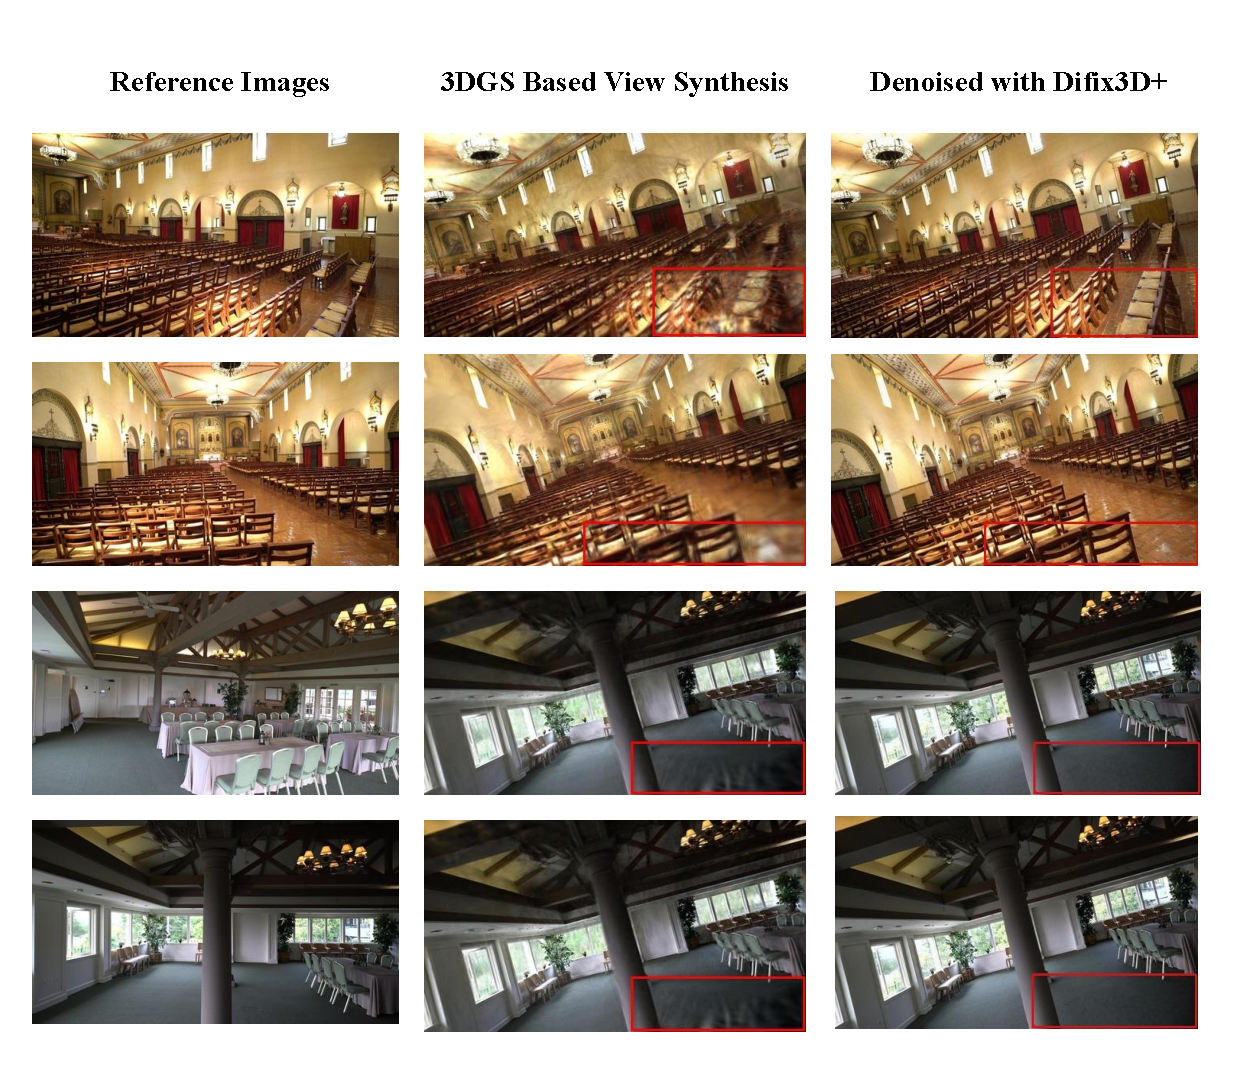
\includegraphics[width=0.98\linewidth,height=0.88\textheight,keepaspectratio]{supplementary_figures/difix3d_examples/difix-2-1.pdf}
\caption{\textbf{Effect of Difix3D denoising on 3DGS-based rotated view synthesis.} Reference images (left), 3DGS-synthesized views (middle), and their denoised counterparts (right), shown for the \textit{Church} and \textit{Meetingroom} scenes from Tanks and Temples. Red boxes mark artifacts in the synthesized views, with corresponding regions in the denoised views to indicate that the artifacts are removed or reduced.}
\label{fig:denoise-examples-2}

\end{figure}

\begin{figure}[!htb]
    \centering
    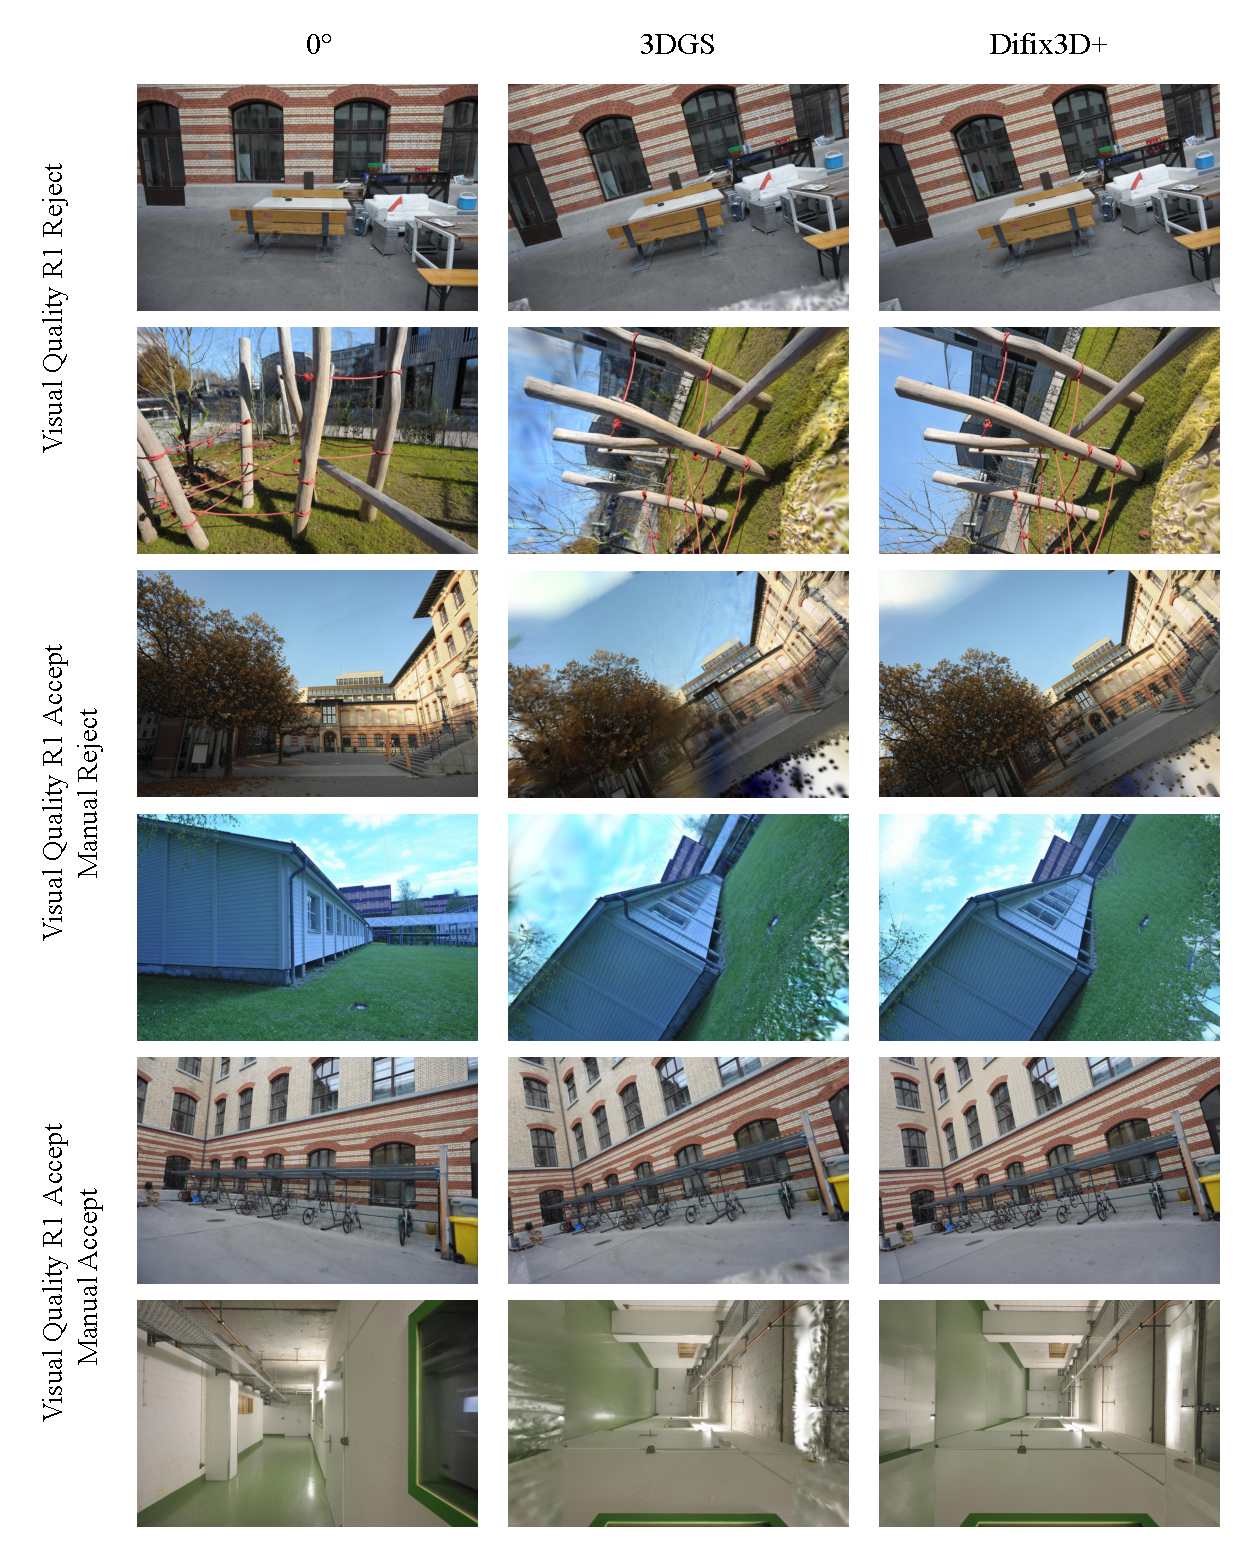
\includegraphics[width=\linewidth,height=0.9\textheight,keepaspectratio]{supplementary_figures/Section_H/SectionH.pdf}
    \caption{Qualitative examples of the quality filtering pipeline across reference ($0^\circ$), raw 3DGS, and Difix-denoised views, showing automated rejections (top), manual rejections (middle), and accepted views (bottom).}
    \label{fig:quality-filtering}
\end{figure}

\section{Failure Case}
\Cref{tab:office_pose} reports pose and point-cloud metrics on ETH3D on the scene \emph{office}. Across other scenes, variance-based roll correction recovers the upright prior and improves the reconstruction, but the \emph{office} scene is a consistent failure case: correction degrades \emph{every} metric for \emph{every} model relative to the baseline. ATE increases uniformly (e.g., $0.040$ to $0.095$ for VGGT-$\Omega$), and both Tacc@30 and Racc@30 fall sharply (e.g., $98.39$ to $63.72$ and $100.00$ to $81.57$ for DA3).

We attribute this failure to rotation to symmetry failure and primarily rotation in pitch and yaw.\Cref{fig:office_failure_qualitative} qualitatively compares the original upright ($0^\circ$) views with the ROVER-corrected views obtained from the corresponding rotated inputs.

\begin{table}[tbp]
\centering
\setlength{\tabcolsep}{3pt}
\caption{Pose estimation results on the ETH3D \emph{office} scene.}
\label{tab:office_pose}
\begin{tabular}{lcccccc}
\toprule
\multirow{2}{*}{Model} & \multicolumn{2}{c}{ATE $\downarrow$} & \multicolumn{2}{c}{Tacc@30 $\uparrow$} & \multicolumn{2}{c}{Racc@30 $\uparrow$} \\
\cmidrule(lr){2-3} \cmidrule(lr){4-5} \cmidrule(lr){6-7}
 & Base & Ours & Base & Ours & Base & Ours \\
\midrule
DA3           & \textbf{0.049} & 0.265 & \textbf{98.39} & 63.72 & \textbf{100.00} & 81.57 \\
MapA          & \textbf{0.236} & 0.313 & \textbf{25.89} & 19.41 & \textbf{92.68}  & 66.75 \\
$\pi^3$       & \textbf{0.208} & 0.326 & \textbf{54.63} & 33.56 & \textbf{92.68}  & 56.40 \\
VGGT          & \textbf{0.157} & 0.241 & \textbf{77.38} & 57.05 & \textbf{92.68}  & 69.49 \\
VGGT-$\Omega$ & \textbf{0.040} & 0.095 & \textbf{96.18} & 86.54 & \textbf{100.00} & 87.50 \\
\bottomrule
\end{tabular}
\end{table}
\raggedbottom
\begin{figure}[H]
    \centering
    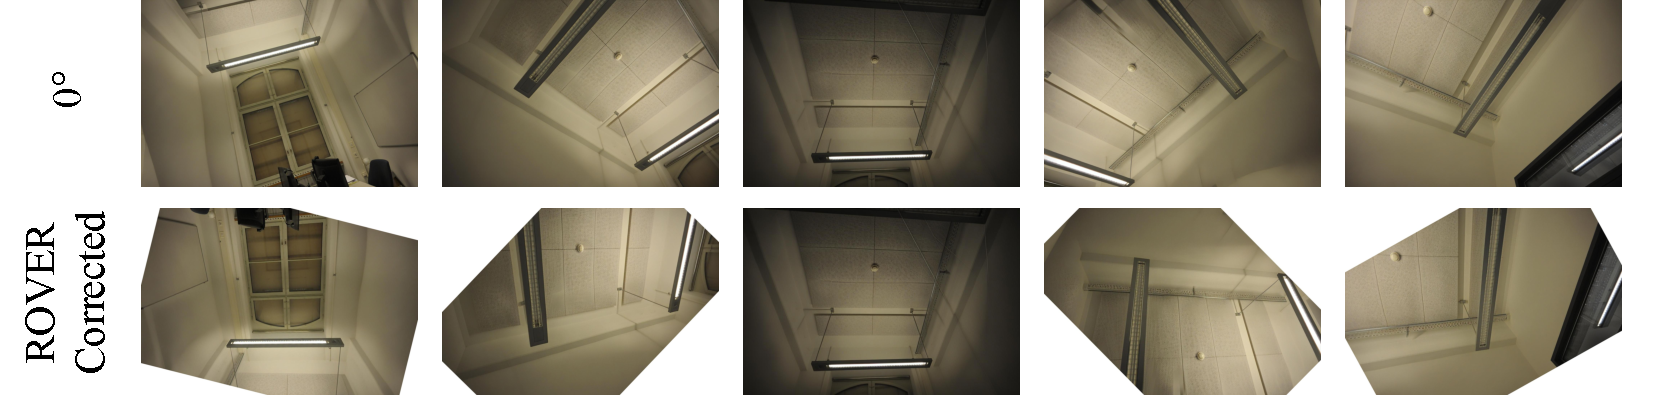
\includegraphics[width=\linewidth, keepaspectratio]{supplementary_figures/eth3d_failcases.pdf}
    \caption{Qualitative failure on the ETH3D \emph{office} scene. Steep upward pitch and ceiling symmetries cause ROVER to introduce spurious corrective rotations to already-upright ($0^\circ$) views.}
    \label{fig:office_failure_qualitative}
\end{figure}

\section{Evaluation Criteria}
\flushbottom
\label{sec:eval_criteria}

Following the protocol described in ~\Cref{sec:algorithm} to generate multi-view scenes with random rotation across frames. We follow the evaluation protocol from \cite{wang2025pi} and evaluate camera pose and point cloud for each rotation configuration set.

\paragraph{Ground-truth pose under roll.}
Let $R$ and $t$ be the $SO(3)$ ground truth rotation matrix and translation vector respectively for a frame. For a roll of $\theta$ about the optical axis, let $\mathbf{R}_z(\theta)$ be the $SO(3)$ rotation matrix about the $z-$axis. Then, under a roll of $\theta$, the world-to-camera pose $[\mathbf{R} \mid \mathbf{t}]$ becomes
$\hat{\mathbf{R}} = \mathbf{R}_z(\theta)\mathbf{R}$ and
$\hat{\mathbf{t}} = \mathbf{R}_z(\theta)\mathbf{t}$. The camera centre
is unchanged,
%
\begin{equation}
-\hat{\mathbf{R}}^{\top}\hat{\mathbf{t}}
= -\mathbf{R}^{\top}\mathbf{R}_z(\theta)^{\top}
   \mathbf{R}_z(\theta)\,\mathbf{t}
= -\mathbf{R}^{\top}\mathbf{t} ,
\label{eq:centre-invariance}
\end{equation}
%
so the ground-truth trajectory is identical to the upright one for
every rotation budget $k$ and angle assignment; the reported ATE
degradation reflects the predicted trajectory alone. Relative
rotations, by contrast, are genuinely re-oriented, so rotation related metrics
are evaluated against altered targets.

\paragraph{Ground-truth geometry under roll.}
Some datasets like ETH3D and DTU provide ground-truth geometry only for the upright
($0^{\circ}$) configuration. Since the scene itself is unchanged by
the roll, we adjust the \emph{support} of the ground truth rather than
its content: the ground-truth depth map $\mathbf{D}$ is rotated in the
image plane, $\hat{\mathbf{D}} = \mathbf{R}_z(\theta)\mathbf{D}$,
regions falling outside the frame after rotation are masked out, and
the remaining pixels are unprojected to 3D using the rotated camera
$[\hat{\mathbf{R}} \mid \hat{\mathbf{t}}]$. This yields the ground-truth
point cloud restricted to the region actually visible in the rotated
view, so that predictions are never penalised for geometry outside the
rolled frustum.

For datasets without ground-truth geometry (Mip-NeRF 360,
RotMV) we take the model's own upright
reconstruction $\hat{\mathbf{P}}_0$ as reference and report the
post-alignment discrepancy of each rotated reconstruction
$\hat{\mathbf{P}}_k$ against it. For our hand-captured dataset no
ground-truth poses are available; we run VGGT on the upright capture
to obtain reference poses and derive the ground truth for each rotated
configuration by composing these with the known roll matrices as in
\eqref{eq:centre-invariance}. These two protocols measure degradation
relative to the model's own upright output rather than absolute
accuracy; our absolute-ground-truth results on 7-Scenes, NRGB-D, ETH3D
and DTU establish the corresponding absolute claims.

\paragraph{Alignment.}
Feed-forward predictions are defined only up to a global similarity
transform. For pose metrics we align the predicted camera centres to
the ground-truth centres with Umeyama. For point
cloud metrics we apply Umeyama followed by ICP to align the predicted
point cloud to the ground truth, following the protocol of
$\pi^3$. All metrics are computed after
alignment.


\paragraph{Pose metrics.}
Let $\mathbf{T}_i, \hat{\mathbf{T}}_i \in SE(3)$ denote the
ground-truth and predicted extrinsics of view $i$, with camera
centres $\mathbf{C}_i, \hat{\mathbf{C}}_i$. After a $\mathrm{Sim}(3)$
trajectory alignment the absolute
trajectory error is
%
\begin{equation}
\mathrm{ATE} = \Big(\tfrac{1}{N}\textstyle\sum_{i=1}^{N}
\big\|\mathbf{C}_i - \hat{\mathbf{C}}_i\big\|_2^2\Big)^{1/2}.
\end{equation}
%
For each of the $\binom{N}{2}$ image pairs $(i,j)$ we form the
relative pose $\Delta\mathbf{T}_{ij} = \mathbf{T}_j\mathbf{T}_i^{-1}$
(and $\Delta\hat{\mathbf{T}}_{ij}$ analogously from
$\hat{\mathbf{T}}_i,\hat{\mathbf{T}}_j$), decomposed into rotation
$\Delta\mathbf{R}_{ij}$ and translation $\mathbf{t}_{ij}$. The
relative rotation error is the geodesic distance
%
\begin{equation}
e^{R}_{ij} = \arccos\!\left(\frac{\mathrm{Tr}\big(\Delta\mathbf{R}_{ij}^{\top}\Delta\hat{\mathbf{R}}_{ij}\big) - 1}{2}\right),
\end{equation}
%
and the relative translation error is the undirected angle between
translation directions (antipodal directions are equivalent, since
scale and sign are unobservable per pair),
%
\begin{equation}
e^{T}_{ij} = \arccos\!\left(\frac{\big|\mathbf{t}_{ij}^{\top}\hat{\mathbf{t}}_{ij}\big|}{\|\mathbf{t}_{ij}\|\,\|\hat{\mathbf{t}}_{ij}\|}\right).
\end{equation}
%

The reported percentages are obtained by thresholding these per-pair errors: $\mathrm{RAcc}_{\tau}$ and $\mathrm{TAcc}_{\tau}$ (Relative Rotation/Translation Accuracy) are the fraction of pairs whose error falls below an angular tolerance $\tau$,
$$\mathrm{RAcc}_{\tau} = \frac{100}{\binom{N}{2}}\sum_{i<j} \mathbbm{1}\left[e^{R}_{ij} < \tau\right], \qquad \mathrm{TAcc}_{\tau} = \frac{100}{\binom{N}{2}}\sum_{i<j} \mathbbm{1}\left[e^{T}_{ij} < \tau\right],$$
reported as percentages; we use $\tau=30^{\circ}$ in the  tables.
The reported AUC uses the \emph{joint} per-pair error
$e^{RT}_{ij} = \max\!\left(e^{R}_{ij}, e^{T}_{ij}\right)$, thresholded
exactly as $\mathrm{RAcc}_\tau$/$\mathrm{TAcc}_\tau$ above,
%
\begin{equation}
\mathrm{Acc}^{\mathrm{joint}}_\tau = \frac{100}{\binom{N}{2}}\sum_{i<j}
\mathbbm{1}\left[e^{RT}_{ij} < \tau\right].
\end{equation}
%
$\mathrm{AUC@}\tau_{\max}$ is the mean of this joint accuracy over
every integer-degree threshold up to $\tau_{\max}$ — a discrete
Riemann-sum approximation, at $1^{\circ}$ resolution, of the area
under the accuracy-vs-threshold curve on $[0^{\circ}, \tau_{\max}]$,
normalised so a perfect predictor scores $100$:
%
\begin{equation}
\mathrm{AUC@}\tau_{\max} = \frac{1}{\tau_{\max}}
\sum_{\tau=1}^{\tau_{\max}} \mathrm{Acc}^{\mathrm{joint}}_\tau .
\end{equation}
%
We report $\mathrm{AUC@30}$ (i.e. $\tau_{\max}=30^{\circ}$) in the
main tables.

\paragraph{Point cloud metrics.}
Following evaluation protocol of $\pi^3$\citep{wang2025pi}, predicted point
maps are aligned to the ground truth with a closed-form
$\mathrm{Sim}(3)$ transform (Umeyama), computed directly from the
pixel-wise correspondence between predicted and ground-truth point
maps, then refined with point-to-point ICP (correspondence threshold
$0.1$--$1.0\,\mathrm{m}$, scaled to each dataset's depth range). Let
$\mathcal{P}$ denote the resulting aligned predicted point cloud and
$\mathcal{Q}$ the ground truth. Accuracy and completeness are the
mean one-sided nearest-neighbour distances,
%
\begin{align}
\mathrm{Acc} &= \tfrac{1}{|\mathcal{P}|}\textstyle\sum_{\mathbf{p}\in\mathcal{P}}
\min_{\mathbf{q}\in\mathcal{Q}}\|\mathbf{p}-\mathbf{q}\|_2 ,
\\[2pt]
\mathrm{Comp} &= \tfrac{1}{|\mathcal{Q}|}\textstyle\sum_{\mathbf{q}\in\mathcal{Q}}
\min_{\mathbf{p}\in\mathcal{P}}\|\mathbf{p}-\mathbf{q}\|_2 ,
\end{align}
%
and their average is the well known Chamfer distance.
Normal consistency (N.C.) is likewise two-sided, averaging the mean absolute
alignment of surface normals at nearest-neighbour correspondences in
each direction,
%
\begin{align}
\mathrm{NC}_1 &= \tfrac{1}{|\mathcal{P}|}\textstyle\sum_{\mathbf{p}\in\mathcal{P}}
\big|\mathbf{n}_{\mathbf{p}} \cdot \mathbf{n}_{\mathrm{nn}_{\mathcal{Q}}(\mathbf{p})}\big| ,
\\[2pt]
\mathrm{NC}_2 &= \tfrac{1}{|\mathcal{Q}|}\textstyle\sum_{\mathbf{q}\in\mathcal{Q}}
\big|\mathbf{n}_{\mathbf{q}} \cdot \mathbf{n}_{\mathrm{nn}_{\mathcal{P}}(\mathbf{q})}\big| ,
\end{align}
%
where $\mathrm{nn}_{\mathcal{X}}(\mathbf{v}) = \arg\min_{\mathbf{x}\in\mathcal{X}}\|\mathbf{v}-\mathbf{x}\|_2$
denotes the nearest neighbour of $\mathbf{v}$ in point set $\mathcal{X}$ (reusing the
correspondences already computed for Acc/Comp above), and $\mathbf{n}_{(\cdot)}$
denotes the surface normal estimated at each point from its local neighbourhood.
We report
\begin{equation}
\mathrm{NC} = \tfrac{1}{2}(\mathrm{NC}_1 + \mathrm{NC}_2) \in [0,1],
\end{equation}
with $\mathrm{NC}=1$ indicating perfectly consistent surface orientation between
prediction and ground truth, and $\mathrm{NC}=0$ indicating orthogonal (maximally
inconsistent) surfaces.



\section{Training Data re-balancing}
\label{sec:training_data_rebalancing}

\Cref{tab:training_data} presents a comprehensive audit of 
the training corpora of all evaluated models. Datasets used by these models are CO3D\citep{co3dv1,reizenstein21co3dv2}, ScanNet/ScanNet++\citep{dai2017scannet, yeshwanthliu2023scannetpp}, MegaDepth\citep{MegaDepthLi18}, DL3DV-10K\citep{ling2024dl3dv}, ARKitScenes\citep{baruch2021arkitscenes}, Mapillary\citep{MapillaryPlanetScaleDepth}, HyperSim\citep{roberts:2021Hypersim}, Habitat/Replica\citep{ramakrishnan2021hm3dhabitat}, Virtual KITTI\citep{gaidon2016virtualkitti2}, BlendedMVS\citep{yao2020blendedmvs}, WildRGB-D\citep{xia2024wildrgbd}, PointOdyssey\citep{zheng2023pointoddessey}, Taskonomy\citep{taskonomy2018}, Waymo Open\cite{Sun_2020_CVPRwaymoopen}, MegaSynth\cite{jiang2024megasynth}, MVS-Synth\citep{DeepMVSSynth}, UnrealStereo4K\citep{zhang2018unrealstereo}, MatrixCity\citep{li2023matrixcity}, Aria Series\citep{pan2023ariadigitaltwin, banerjee2024ariaHOT3D, ma2024arianymeriadataset, lv2024ariaeverydayactivities}, Dynamic Replica\citep{karaev2023dynamicreplicastereo}, Spring\citep{mehl2023springdataset}, Structured3D\citep{Structured3Ddataset}, Cityscapes\cite{cordts2016cityscapes}, GTA-SfM\citep{cao2020longgtasfm}, Kubric\citep{greff2021kubricdataset}, TartanAir\citep{tartanair2020iros} and Mid-Air \citep{Fonder2019MidAir} datasets. Across \textbf{27} datasets spanning indoor RGB-D scans, outdoor photo collections, driving sequences, and synthetic renderings, the overwhelming majority are upright by construction with each model trained on between 10 and 19 fully upright datasets and at most 2 partially aligned ones. This confirms that UprightBias is a data-driven phenomenon: feed-forward models inadvertently absorb a strong canonical orientation prior simply by virtue of what their training data looks like.
\begin{table}[t]
\centering
\caption{Training datasets used by each feed-forward geometric model and their upright alignment status. \checkmark~=~fully upright; $\sim$~=~partially upright The overwhelming majority of training data across all models is upright by construction}
\label{tab:training_data}
\small
\resizebox{\linewidth}{!}{
\begin{tabular}{llccccccc}
\toprule
\textbf{Dataset} & 
\textbf{Capture Modality} & 
\textbf{Upright} & 
\textbf{VGGT} & 
\textbf{VGGT-$\Omega$} & 
\textbf{DA3} & 
\textbf{MapA.} & 
\textbf{$\pi^3$} \\
\midrule
CO3D               & Handheld object-centric video      & \checkmark & \checkmark & \checkmark & \checkmark &            & \checkmark \\
ScanNet / ScanNet++  & Handheld RGB-D indoor scan         & \checkmark & \checkmark & \checkmark & \checkmark & \checkmark & \checkmark \\
MegaDepth            & Internet landmark photography      & \checkmark & \checkmark & \checkmark & \checkmark & \checkmark & \checkmark \\
DL3DV-10K            & Scene-level video                  & \checkmark & \checkmark & \checkmark & \checkmark & \checkmark &            \\
ARKitScenes          & iPad indoor capture                & \checkmark &            & \checkmark & \checkmark &            & \checkmark \\
Mapillary            & Street-level vehicle camera        & \checkmark & \checkmark & \checkmark &            & \checkmark &            \\
HyperSim             & Synthetic indoor rendering         & \checkmark & \checkmark & \checkmark & \checkmark &            & \checkmark \\
Habitat / Replica    & Simulated indoor environments      & \checkmark & \checkmark & \checkmark & \checkmark &            & \checkmark \\
Virtual KITTI        & Driving simulation                 & \checkmark & \checkmark & \checkmark & \checkmark &            &            \\
BlendedMVS           & SfM outdoor/indoor photos          & \checkmark & \checkmark &            & \checkmark & \checkmark & \checkmark \\
WildRGB-D            & In-the-wild RGBD video             & \checkmark & \checkmark & \checkmark & \checkmark &            & \checkmark \\
PointOdyssey         & Synthetic ground-level motion      & \checkmark & \checkmark & \checkmark & \checkmark &            &            \\
Taskonomy            & Indoor scene photography           & \checkmark &            & \checkmark & \checkmark &            & \checkmark \\
Waymo Open               & Autonomous driving cameras         & \checkmark &            & \checkmark & \checkmark &            &            \\
MegaSynth            & Synthetic scene rendering          & \checkmark &            & \checkmark & \checkmark &            &            \\
MVS-Synth            & Synthetic multi-view stereo        & \checkmark & \checkmark & \checkmark & \checkmark & \checkmark &            \\
UnrealStereo4K       & Synthetic indoor/outdoor           & \checkmark &            & \checkmark & \checkmark & \checkmark &            \\
MatrixCity           & Synthetic city aerial/ground       & \checkmark &            &            & \checkmark &            & \checkmark \\
Aria Series          & Egocentric wearable capture        & \checkmark & \checkmark & \checkmark &            & \checkmark &            \\
Dynamic Replica      & Synthetic dynamic indoor           & \checkmark &            & \checkmark &            & \checkmark &            \\
Spring               & Synthetic outdoor driving          & \checkmark &            &            &            & \checkmark &            \\
Structured3D         & Synthetic indoor rendering         & \checkmark &            &            & \checkmark &            &            \\
Cityscapes           & Driving forward-facing camera      & \checkmark &            &            & \checkmark &            &            \\
GTA-SfM              & Game engine driving scenes         & \checkmark &            &            &            &            & \checkmark \\
\midrule
Kubric               & Synthetic random viewpoints        & $\sim$     & \checkmark &            &            &            &            \\
TartanAir            & Drone and aerial simulation        & $\sim$     &            & \checkmark & \checkmark &            & \checkmark \\
Mid-Air              & Drone aerial footage               & $\sim$     &            & \checkmark &            &            & \checkmark \\
\midrule
\multicolumn{2}{l}{\textbf{Fully upright datasets used}} 
& & \textbf{13} & \textbf{18} & \textbf{19} & \textbf{10} & \textbf{11} \\
\multicolumn{2}{l}{\textbf{Partially upright datasets used}} 
& & \textbf{1} & \textbf{2} & \textbf{1} & \textbf{0} & \textbf{2} \\
\bottomrule
\end{tabular}
}
\end{table}
To investigate if re-balancing the training data and finetuning the model recovers the performance we fine-tune $\pi^3$ on a re-balanced version of the DTU training set 
augmented with randomly rotated multi-view sequences, and evaluate 
on the DTU test set under the same rotated-input protocol used 
throughout the paper. Tables~\Cref{tab:pointmap_pi3_variants_dtu} 
and~\Cref{tab:pose_pi3_variants_dtu} report point-map and camera 
pose metrics respectively for the pretrained and fine-tuned models 
across four test scenes. The results do not support the re-balancing hypothesis. 
Fine-tuning yields inconsistent changes, consistent with the feature-distortion risk discussed in \Cref{sec:ROVER_detail}\citep{kumar2022finetuningchallenges, tang2020longchallenges, kang2019decouplingtrainingdata3}. More specifically fine-tuning on rotated data disrupts the DINOv2-derived visual representations that $\pi^3$ relies on, as the rotated fine-tuning distribution diverges from the DINOv2 pretraining distribution. 

% \newcommand{\result}[2]{%
%   \makecell{#1\\[-2pt]{\scriptsize $\pm$#2}}%
% }

% \newcommand{\bestresult}[2]{%
%   \makecell{\bfseries #1\\[-2pt]{\scriptsize $\mathbf{\pm #2}$}}%
% }

% \begin{table}[H]
% \centering
% \caption{
% DTU test-scene point-cloud metrics for the $\pi^3$ backbone.
% Results are reported as mean $\pm$ standard deviation over 50 rotation
% sets per scene. PT denotes pretrained, PT+VC applies DINOv2 variance
% correction, and FT denotes finetuning (v2). Best results are bold.
% }
% \label{tab:pointmap_pi3_variants_dtu}

% \setlength{\tabcolsep}{4.2pt}
% \renewcommand{\arraystretch}{1.12}
% \small

% \begin{tabular}{l ccc ccc ccc}
% \toprule
% \multirow{2}{*}{Scene}
% & \multicolumn{3}{c}{Accuracy $\downarrow$}
% & \multicolumn{3}{c}{Completeness $\downarrow$}
% & \multicolumn{3}{c}{Normal Consistency $\uparrow$} \\
% \cmidrule(lr){2-4}
% \cmidrule(lr){5-7}
% \cmidrule(lr){8-10}
% & PT & PT+VC(Ours) & FT
% & PT & PT+VC(Ours) & FT
% & PT & PT+VC(Ours) & FT \\
% \midrule    

% scan1
% & \result{0.923}{0.311}
% & \bestresult{0.797}{0.269}
% & \result{2.251}{0.279}
% & \result{0.902}{0.281}
% & \bestresult{0.828}{0.238}
% & \result{1.347}{0.161}
% & \result{0.646}{0.009}
% & \result{0.643}{0.007}
% & \bestresult{0.652}{0.006}
% \\

% scan10
% & \result{5.701}{6.254}
% & \result{5.044}{5.790}
% & \bestresult{4.340}{1.000}
% & \result{4.463}{9.323}
% & \bestresult{3.511}{6.707}
% & \result{4.057}{0.704}
% & \result{0.655}{0.020}
% & \result{0.652}{0.022}
% & \bestresult{0.681}{0.013}
% \\

% scan118
% & \result{3.384}{2.605}
% & \result{1.841}{1.423}
% & \bestresult{1.467}{0.272}
% & \result{5.969}{9.243}
% & \result{3.183}{7.865}
% & \bestresult{1.493}{0.286}
% & \result{0.593}{0.039}
% & \bestresult{0.610}{0.028}
% & \result{0.608}{0.004}
% \\

% scan77
% & \bestresult{5.962}{1.011}
% & \result{6.149}{1.069}
% & \result{7.931}{1.186}
% & \bestresult{6.658}{1.894}
% & \result{6.938}{1.831}
% & \result{12.447}{2.721}
% & \result{0.622}{0.010}
% & \bestresult{0.628}{0.012}
% & \result{0.607}{0.007}
% \\

% \bottomrule
% \end{tabular}
% \end{table}

%%%%%%%%%%%%%%%%%%%%%%%%%%%%%%%%%%%%%%%%%%%%%%%%%%%%%%%%%%%%%%%%%%%%%%%%%%%%%%%%%%%%%%%%%%%%%%%%%%%%%%%%%%%%%%%%%%%%%%%%%%%%%%%%%%%%%%%%%%%%%%%%%%%%%%%%%%%%%%%%%%%%%%%%%%%%%%%%%%%%%%%%%%%%%%%%%%%%%%%%%%%%%%%%%%%%%%%%%%%%%%%%%%%%%%%%%%%%%%%%

\newcommand{\result}[2]{%
  \makecell{#1\\[-2pt]{\scriptsize $\pm$#2}}%
}

\newcommand{\bestresult}[2]{%
  \makecell{\bfseries #1\\[-2pt]{\scriptsize $\mathbf{\pm #2}$}}%
}

\begin{table}[H]
\centering
\caption{
DTU test-scene point-cloud metrics for the $\pi^3$ backbone finetuning with rebalanced dataset.
Results are reported as mean $\pm$ standard deviation over 50 rotation
sets per scene. We compare the pretrained model with the finetuned
model.
}
\label{tab:pointmap_pi3_variants_dtu}

\setlength{\tabcolsep}{4.2pt}
\renewcommand{\arraystretch}{1.12}
\small

\begin{tabular}{l cc cc cc}
\toprule
\multirow{2}{*}{Scene}
& \multicolumn{2}{c}{Accuracy $\downarrow$}
& \multicolumn{2}{c}{Completeness $\downarrow$}
& \multicolumn{2}{c}{Normal Consistency $\uparrow$} \\
\cmidrule(lr){2-3}
\cmidrule(lr){4-5}
\cmidrule(lr){6-7}
& Pretrained & Finetuned
& Pretrained & Finetuned
& Pretrained & Finetuned \\
\midrule    

scan1
& \bestresult{0.923}{0.311}
& \result{2.251}{0.279}
& \bestresult{0.902}{0.281}
& \result{1.347}{0.161}
& \result{0.646}{0.009}
& \bestresult{0.652}{0.006}
\\

scan10
& \result{5.701}{6.254}
& \bestresult{4.340}{1.000}
& \result{4.463}{9.323}
& \bestresult{4.057}{0.704}
& \result{0.655}{0.020}
& \bestresult{0.681}{0.013}
\\

scan118
& \result{3.384}{2.605}
& \bestresult{1.467}{0.272}
& \result{5.969}{9.243}
& \bestresult{1.493}{0.286}
& \result{0.593}{0.039}
& \bestresult{0.608}{0.004}
\\

scan77
& \bestresult{5.962}{1.011}
& \result{7.931}{1.186}
& \bestresult{6.658}{1.894}
& \result{12.447}{2.721}
& \bestresult{0.622}{0.010}
& \result{0.607}{0.007}
\\

\bottomrule
\end{tabular}
\end{table}
% \begin{table}[H]
% \centering

% % Local result-cell definitions
% \def\result#1#2{%
%   \makecell{#1\\[-2pt]{\scriptsize $\pm$#2}}%
% }
% \def\bestresult#1#2{%
%   \makecell{\bfseries #1\\[-2pt]{\scriptsize $\mathbf{\pm #2}$}}%
% }

% \caption{
% DTU test-scene pose metrics for the $\pi^3$ backbone.
% Results are reported as mean $\pm$ standard deviation over 50 rotation
% sets per scene. PT denotes pretrained, PT+VC applies DINOv2 variance
% correction, and FT denotes finetuning (v2). Best results are bold.
% }
% \label{tab:pose_pi3_variants_dtu}

% \setlength{\tabcolsep}{7pt}
% \renewcommand{\arraystretch}{1.12}
% \small

% \begin{tabular}{l ccc ccc}
% \toprule
% \multirow{2}{*}{Scene}
% & \multicolumn{3}{c}{ATE $\downarrow$}
% & \multicolumn{3}{c}{AUC@30 $\uparrow$} \\
% \cmidrule(lr){2-4}
% \cmidrule(lr){5-7}
% & PT & PT+VC(Ours) & FT
% & PT & PT+VC(Ours) & FT \\
% \midrule

% scan1
% & \result{9.161}{3.658}
% & \bestresult{6.805}{2.481}
% & \result{10.550}{3.293}
% & \result{94.832}{2.343}
% & \bestresult{96.351}{1.534}
% & \result{94.073}{1.927}
% \\

% scan10
% & \result{72.433}{77.302}
% & \result{64.940}{61.045}
% & \bestresult{34.919}{4.356}
% & \result{77.543}{18.736}
% & \bestresult{78.684}{13.282}
% & \result{61.702}{3.774}
% \\

% scan118
% & \result{79.647}{88.556}
% & \result{37.851}{65.303}
% & \bestresult{17.696}{3.658}
% & \result{81.022}{17.060}
% & \bestresult{90.468}{5.708}
% & \result{86.688}{3.347}
% \\

% scan77
% & \result{49.597}{41.676}
% & \bestresult{39.541}{43.088}
% & \result{206.479}{64.354}
% & \result{77.976}{12.527}
% & \bestresult{84.647}{6.890}
% & \result{26.733}{9.703}
% \\

% \bottomrule
% \end{tabular}
% \end{table}


%%%%%%%%%%%%%%%%%%%%%%%%%%%%%%%%%%%%%%%%%%%%%%%%%%%%%%%%%%%%%%%%%%%%%%%%%%%%%%%%%%%%%%%%%%%%%%%%%%%%%%%%%%%%%%%%%%%%%%


\begin{table}[tbp]
\centering

% Local result-cell definitions
\def\result#1#2{%
  \makecell{#1\\[-2pt]{\scriptsize $\pm$#2}}%
}
\def\bestresult#1#2{%
  \makecell{\bfseries #1\\[-2pt]{\scriptsize $\mathbf{\pm #2}$}}%
}

\caption{
DTU test-scene pose metrics for the $\pi^3$ backbone finetuning with rebalanced dataset.
Results are reported as mean $\pm$ standard deviation over 50 rotation
sets per scene. We compare the pretrained model with the finetuned (v2)
model.
}
\label{tab:pose_pi3_variants_dtu}

\setlength{\tabcolsep}{7pt}
\renewcommand{\arraystretch}{1.12}
\small

\begin{tabular}{l cc cc}
\toprule
\multirow{2}{*}{Scene}
& \multicolumn{2}{c}{ATE $\downarrow$}
& \multicolumn{2}{c}{$\text{AUC}_{30}$ $\uparrow$} \\
\cmidrule(lr){2-3}
\cmidrule(lr){4-5}
& Pretrained & Finetuned
& Pretrained & Finetuned \\
\midrule

scan1
& \bestresult{9.161}{3.658}
& \result{10.550}{3.293}
& \bestresult{94.832}{2.343}
& \result{94.073}{1.927}
\\

scan10
& \result{72.433}{77.302}
& \bestresult{34.919}{4.356}
& \bestresult{77.543}{18.736}
& \result{61.702}{3.774}
\\

scan118
& \result{79.647}{88.556}
& \bestresult{17.696}{3.658}
& \result{81.022}{17.060}
& \bestresult{86.688}{3.347}
\\

scan77
& \bestresult{49.597}{41.676}
& \result{206.479}{64.354}
& \bestresult{77.976}{12.527}
& \result{26.733}{9.703}
\\

\bottomrule
\end{tabular}
\end{table}


\section{Outlier Detection using RobustVGGT}
\label{sec:outlier_detection_robustvggt}

% \section{Relational Feature and Attention-Based Rotation Identification}
% \label{sec:attentionbased_rotation_detection}

% In-plane frame rotations disrupt spatial feature correlations in feed-forward models, degrading camera pose estimation.
% Inspired by RobustVGGT~\citep{robustvggt}, we identify rotated frames in a zero-shot manner directly from internal network features. Specifically, we extract spatial patch tokens $\mathbf{X}_i \in \mathbb{R}^{P \times D}$ and multi-head query-key projections $\mathbf{Q}_i, \mathbf{K}_i \in \mathbb{R}^{H \times P \times d_k}$ from the first global self-attention layer across an $N$-frame sequence during a single forward pass.

% \subsection{Relational Representation Matrix}
% For each frame pair $(i, j)$, we evaluate inter-frame consistency through token similarity and global attention:
% \begin{equation}
% C_{i,j} = \frac{1}{P^2} \sum_{p,q=1}^{P} \frac{\langle \mathbf{X}_{i,p}, \mathbf{X}_{j,q} \rangle}{\|\mathbf{X}_{i,p}\|_2 \|\mathbf{X}_{j,q}\|_2}, \qquad
% A_{i,j} = \frac{1}{H P} \sum_{h=1}^{H} \sum_{p=1}^{P} \operatorname{Softmax}\left( \frac{\mathbf{Q}_{i,p}^{(h)} (\mathbf{K}_j^{(h)})^\top}{\sqrt{d_k}} \right).
% \end{equation}
% Both matrices are min-max normalized to $[0, 1]$ across all frame pairs using a small constant $\epsilon = 10^{-6}$ for numerical stability, yielding normalized matrices $\mathbf{C}'$ and $\mathbf{A}'$. We construct the joint symmetric affinity matrix as $\mathbf{M} = \frac{1}{2}(\mathbf{C}' + \mathbf{A}') \in \mathbb{R}^{N \times N}$.

% \subsection{Sequence-Level Rotation Detection}
% To detect orientation anomalies, we define a sequence reference profile $\mathbf{T} \in \mathbb{R}^N$ by taking the column-wise median across frames, $T_j = \operatorname{median}_{i}(M_{i,j})$, and compute each frame's mean absolute deviation:
% \begin{equation}
% d_i = \frac{1}{N} \sum_{j=1}^{N} |M_{i,j} - T_j|.
% \end{equation}
% Frames are sorted in descending order of deviation: $\mathbf{d}_{\text{sorted}} = [d_{\pi(1)}, \dots, d_{\pi(N)}]$. We partition the sequence under two orientation priors:
% \begin{itemize}
%     \item \textbf{Minority Rotation (Gap-Based):} Assuming rotated frames form an anomalous minority ($k \le \lfloor N/2 \rfloor$), the decision boundary is placed at the largest consecutive deviation drop:
%     \begin{equation}
%     k^* = \arg\max_{1 \le k \le \lfloor N/2 \rfloor} (d_{\pi(k)} - d_{\pi(k+1)}).
%     \end{equation}
%     The top $k^*$ frames $\{\pi(1), \dots, \pi(k^*)\}$ are classified as \textbf{rotated}, while the remaining $N - k^*$ frames are labeled as \textbf{upright}.

%     \item \textbf{Majority Rotation (Variance Minimization):} When rotated frames dominate, the reference profile $\mathbf{T}$ reflects the rotated orientation, making upright frames appear as high-deviation outliers. We partition the sequence into candidate upright frames $G_{\text{up}} = \{d_{\pi(1)}, \dots, d_{\pi(k)}\}$ and rotated frames $G_{\text{rot}} = \{d_{\pi(k+1)}, \dots, d_{\pi(N)}\}$. Sweeping $k \in [1, \min(8, N-1)]$, the optimal split $k^*$ minimizes the within-class variance:
%     \begin{equation}
%     \sigma^2_w(k) = \frac{k}{N} \sigma^2(G_{\text{up}}) + \frac{N - k}{N} \sigma^2(G_{\text{rot}}).
%     \end{equation}
%     The top $k^*$ frames are isolated as \textbf{upright}, and the remaining $N - k^*$ frames are classified as \textbf{rotated}.
% \end{itemize}

% \subsection{Sensitivity to the Rotation Prior}
% As shown in Table~\Cref{tab:rotation-prior}, detection is substantially more reliable when rotated frames form the minority (average Global F1 of $0.811$ vs.\ $0.543$ under the majority setting). Precision and recall both degrade when canonical reference frames become scarce, demonstrating the necessity of an upright reference anchor for unsupervised relational profiling.
A natural alternative to correcting rotated views is to detect and discard them. As noted in \cref{sec:ablation}, we evaluate this strategy using RobustVGGT~\citep{robustvggt}, which flags views that are inconsistent with the rest of the sequence and excludes them before reconstruction. Unlike ROVER, which estimates the orientation of each view independently, this approach relies on relations between views. Following  RobustVGGT , we identify rotated frames in a zero-shot manner directly from the model's internal feature representations. Specifically, we extract spatial patch tokens $\mathbf{X}_i \in \mathbb{R}^{N_p \times D_{\text{feat}}}$ and multi-head query-key projections $\mathbf{Q}_i, \mathbf{K}_i \in \mathbb{R}^{H \times N_p \times d_k}$ from the first global self-attention layer across an $N$-frame sequence during a single forward pass.

\subsection{Relational Representation Matrix}
For each frame pair $(i, j)$, we evaluate inter-frame consistency through token similarity and global attention:
\begin{equation}
S_{i,j} = \frac{1}{N_p^2} \sum_{u,v=1}^{N_p} \frac{\langle \mathbf{X}_{i,u}, \mathbf{X}_{j,v} \rangle}{\|\mathbf{X}_{i,u}\|_2 \|\mathbf{X}_{j,v}\|_2}, \qquad
A_{i,j} = \frac{1}{H N_p} \sum_{h=1}^{H} \sum_{u=1}^{N_p} \operatorname{Softmax}\left( \frac{\mathbf{Q}_{i,u}^{(h)} (\mathbf{K}_j^{(h)})^\top}{\sqrt{d_k}} \right).
\end{equation}
Both matrices are min-max normalized to $[0, 1]$ across all frame pairs using a small constant $\epsilon = 10^{-6}$ for numerical stability, yielding normalized matrices $\mathbf{S}'$ and $\mathbf{A}'$. We construct the joint symmetric affinity matrix as $\mathbf{W} = \frac{1}{2}(\mathbf{S}' + \mathbf{A}') \in \mathbb{R}^{N \times N}$.

\subsection{Sequence-Level Rotation Detection}
To detect orientation anomalies, we define a sequence reference profile $\mathbf{r} \in \mathbb{R}^N$ by taking the column-wise median across frames, $r_j = \operatorname{median}_{i}(W_{i,j})$, and compute each frame's mean absolute deviation:
\begin{equation}
d_i = \frac{1}{N} \sum_{j=1}^{N} |W_{i,j} - r_j|.
\end{equation}
Frames are sorted in descending order of deviation: $\mathbf{d}_{\text{sorted}} = [d_{\rho(1)}, \dots, d_{\rho(N)}]$. We partition the sequence under two orientation priors:

$\bullet$ \textbf{Minority Rotation (Gap-Based):} Assuming rotated frames form an anomalous minority ($s \le \lfloor N/2 \rfloor$), the decision boundary is placed at the largest consecutive deviation drop:
    \begin{equation}
    s^* = \arg\max_{1 \le s \le \lfloor N/2 \rfloor} (d_{\rho(s)} - d_{\rho(s+1)}).
    \end{equation}
    The top $s^*$ frames $\{\rho(1), \dots, \rho(s^*)\}$ are classified as \textbf{rotated}, while the remaining $N - s^*$ frames are labeled as \textbf{upright}.

$\bullet$ \textbf{Majority Rotation (Variance Minimization):} When rotated frames dominate, the reference profile $\mathbf{r}$ reflects the rotated orientation, making upright frames appear as high-deviation outliers. We partition the sequence into candidate upright frames $G_{\text{up}} = \{d_{\rho(1)}, \dots, d_{\rho(s)}\}$ and rotated frames $G_{\text{rot}} = \{d_{\rho(s+1)}, \dots, d_{\rho(N)}\}$. Sweeping $s \in [1, \min(8, N-1)]$, the optimal split $s^*$ minimizes the within-class variance:
    \begin{equation}
    \sigma^2_w(s) = \frac{s}{N} \sigma^2(G_{\text{up}}) + \frac{N - s}{N} \sigma^2(G_{\text{rot}}).
    \end{equation}
    The top $s^*$ frames are isolated as \textbf{upright}, and the remaining $N - s^*$ frames are classified as \textbf{rotated}.


\subsection{Sensitivity to the Rotation Prior}
As shown in Table~\Cref{tab:rotation-prior}, detection is substantially more reliable when rotated frames form the minority (average Global F1 of $0.811$ vs.\ $0.543$ under the majority setting). Precision and recall both degrade when canonical reference frames become scarce, demonstrating the necessity of an upright reference anchor for unsupervised image identification

\subsection{Limitations of RobustVGGT}
The approach described in RobustVGGT drops the anomalous frames and predicts a sparse point cloud. Further, it would predict cameras only for the chosen frames. The results in \Cref{tab:rotation-prior} highlight two limitations of rejection based approach in RobustVGGT for handling rotated frames. First, detection depends on upright frames serving as a reference, and becomes unreliable when such frames are scarce. Second, even perfect detection discards the rotated views, reducing coverage of the scene. ROVER avoids both: it estimates the orientation of each view from its own DINOv2 features, independent of the fraction of rotated views, and retains all views after canonicalization. This allows our approach to recover reconstruction quality.

% --- Table placed with [!b] so it anchors to the bottom of the page after Section N.3 ---
\begin{table}[h]
\centering
\caption{Rotation detection performance under minority and majority rotated settings.}
\label{tab:rotation-prior}

\setlength{\tabcolsep}{3.5pt}
\renewcommand{\arraystretch}{0.95}

{\scriptsize
\begin{tabular}{c l ccc ccc}
\toprule
& & \multicolumn{3}{c}{\textbf{Minority Rotated}} & \multicolumn{3}{c}{\textbf{Majority Rotated}} \\
\cmidrule(lr){3-5} \cmidrule(lr){6-8}
\textbf{Dataset} & \textbf{Model} & \textbf{Prec.} $\uparrow$ & \textbf{Rec.} $\uparrow$ & \textbf{F1} $\uparrow$ & \textbf{Prec.} $\uparrow$ & \textbf{Rec.} $\uparrow$ & \textbf{F1} $\uparrow$ \\
\midrule
\multirow{3}{*}{DTU}
& VGGT          & 0.9180 & 0.8127 & 0.8621 & 0.3676 & 0.3452 & 0.3560 \\
& VGGT-$\Omega$ & 0.9144 & 0.8012 & 0.8541 & 0.5239 & 0.4179 & 0.4649 \\
& $\pi^3$           & 0.9067 & 0.8024 & 0.8514 & 0.4168 & 0.3726 & 0.3935 \\
\midrule
\multirow{3}{*}{ETH3D}
& VGGT          & 0.7673 & 0.6183 & 0.6848 & 0.3699 & 0.2847 & 0.3217 \\
& VGGT-$\Omega$ & 0.7604 & 0.6135 & 0.6791 & 0.3608 & 0.3017 & 0.3286 \\
& $\pi^3$           & 0.7545 & 0.6413 & 0.6933 & 0.4014 & 0.6423 & 0.4941 \\
\midrule
\multirow{3}{*}{Mip-NeRF 360}
& VGGT          & 0.9442 & 0.8844 & 0.9133 & 0.8756 & 0.8368 & 0.8558 \\
& VGGT-$\Omega$ & 0.9075 & 0.8394 & 0.8721 & 0.8895 & 0.7655 & 0.8228 \\
& $\pi^3$           & 0.9121 & 0.8594 & 0.8849 & 0.8906 & 0.8130 & 0.8500 \\
\midrule
\textbf{Average} & & \textbf{0.865} & \textbf{0.764} & \textbf{0.811} & \textbf{0.566} & \textbf{0.531} & \textbf{0.543} \\
\bottomrule
\end{tabular}
}
\end{table}


% \subsection{Overview \& Motivation}
% When feed forward models encounter mixed-orientation frames (where in-plane rotations are introduced to individual frames), the out-of-distribution rotation disrupts spatial feature correlation, causing severe pose estimation errors and trajectory drifts.

% To resolve this, we test a self-supervised method to identify rotated frames directly from the network's internal features inspired by RobustVGGT\citep{robustvggt}. By extracting intermediate tokens and query-key attention maps from the global aggregator blocks during a single forward pass, we construct an $N \times N$ relational representation matrix to profile sequence-level orientation patterns. We analyze two clustering algorithms corresponding to two distinct priors:
% \begin{enumerate}
%     \item \textbf{Minority Rotation Detection:} Assumes that upright frames dominate the sequence and rotated frames represent the minority anomaly.
%     \item \textbf{Majority Rotation Detection:} Assumes that rotated frames form the majority of the sequence and upright frames represent the minority anomaly.
% \end{enumerate}

% \subsection{Relational Representation Matrix Construction}
% For a sequence of $N$ image frames, the algorithm extracts intermediate representations from the initial global self-attention layer to capture:
% \begin{itemize}
%     \item \textbf{Token Representations ($\mathbf{X}$):} Let $\mathbf{X}_i \in \mathbb{R}^{P \times D}$ be the spatial patch tokens for frame $i$, where $P$ is the number of tokens per image and $D$ is the feature dimension.
%     \item \textbf{Attention Query ($\mathbf{Q}$) and Key ($\mathbf{K}$) Projections:} Let $\mathbf{Q}_i \in \mathbb{R}^{H \times P \times d_k}$ and $\mathbf{K}_i \in \mathbb{R}^{H \times P \times d_k}$ represent the query and key maps, where $H$ is the number of attention heads.
% \end{itemize}

% For each frame $i$ acting as an ``anchor,'' we compute its relationship to all other frames $j \in [1, N]$ using two normalized metrics:

% \subsubsection{Spatial Token Cosine Similarity Matrix ($C$)}
% For an anchor frame $i$, the spatial similarity vector relative to frame $j$ is computed by taking the average pairwise cosine similarity between their spatial patch features:
% \begin{equation}
% C_{i,j} = \frac{1}{P^2} \sum_{p=1}^{P} \sum_{q=1}^{P} \frac{\langle \mathbf{X}_{i,p}, \mathbf{X}_{j,q} \rangle}{\|\mathbf{X}_{i,p}\|_2 \|\mathbf{X}_{j,q}\|_2}
% \end{equation}
% The raw similarities are then min-max normalized across all frames to establish a range of $[0, 1]$:
% \begin{equation}
% C'_{i,j} = \frac{C_{i,j} - \min_{k} C_{i,k}}{\max_{k} C_{i,k} - \min_{k} C_{i,k} + \epsilon}
% \end{equation}

% \subsubsection{Cross-Image Attention Matrix ($A$)}
% The attention weight assigned by anchor frame $i$ to target frame $j$ is computed from the softmax probabilities of the dot-product attention queries:
% \begin{equation}
% A_{i,j} = \frac{1}{H \cdot P} \sum_{h=1}^{H} \sum_{p=1}^{P} \operatorname{Softmax}\left( \frac{\mathbf{Q}_{i,p}^{(h)} (\mathbf{K}_j^{(h)})^T}{\sqrt{d_k}} \right)
% \end{equation}
% Similarly, the attention scores are min-max normalized:
% \begin{equation}
% A'_{i,j} = \frac{A_{i,j} - \min_{k} A_{i,k}}{\max_{k} A_{i,k} - \min_{k} A_{i,k} + \epsilon}
% \end{equation}

% \subsubsection{Combined Relational Matrix ($M$)}
% To capture both semantic feature similarity and receptive-field attention, we build the final symmetric relational matrix $M \in \mathbb{R}^{N \times N}$:
% \begin{equation}
% M_{i,j} = 0.5 \cdot C'_{i,j} + 0.5 \cdot A'_{i,j}
% \end{equation}


% \subsection{Detection Algorithms}
% Both algorithms convert the relational matrix $M$ into a 1D sequence deviation score. First, they construct a sequence-level ``median template profile'' representing the typical relational behavior of the sequence:
% \begin{equation}
% \mathbf{T} = \operatorname{median}(M, \text{axis}=0)
% \end{equation}
% The absolute deviation of each frame $i$ from the template is computed as:
% \begin{equation}
% d_i = \frac{1}{N} \sum_{j=1}^{N} |M_{i,j} - \mathbf{T}_j|
% \end{equation}
% Frames are then sorted by descending deviation score: $\mathbf{d}_{\text{sorted}} = [d_{\pi(1)}, d_{\pi(2)}, \dots, d_{\pi(N)}]$ where $d_{\pi(1)} \ge d_{\pi(2)} \dots \ge d_{\pi(N)}$.

% \subsubsection{Method A: Gap-Based Minority Clustering}
% This method assumes that \textbf{rotated frames are the minority anomaly}, exhibiting unusually high deviations ($d_i$) relative to the upright template profile.
% \begin{enumerate}
%     \item The differences (gaps) between consecutive sorted deviations are calculated:
%     \begin{equation}
%     g_k = d_{\pi(k)} - d_{\pi(k+1)}, \quad \text{for } k \in [1, N-1]
%     \end{equation}
%     \item Under the minority constraint, no more than half of the frames can be rotated. The search window is restricted to:
%     \begin{equation}
%     k \in \left[1, \left\lfloor \frac{N-1}{2} \right\rfloor\right]
%     \end{equation}
%     \item The cluster boundary is defined at the rank index that maximizes the gap:
%     \begin{equation}
%     k^* = \arg\max_{k} g_k
%     \end{equation}
%     \item The frames corresponding to indices $\{\pi(1), \dots, \pi(k^*)\}$ are classified as \textbf{rotated}.
% \end{enumerate}

% \subsubsection{Method B: Otsu-Style Variance Minimization}
% This method assumes that \textbf{rotated frames are the majority}, and upright frames are the anomalous minority. In this scenario, the template profile $\mathbf{T}$ represents rotated frames, making the upright frames appear as high-deviation anomalies.
% \begin{enumerate}
%     \item A threshold index $k$ is swept from $1$ to $\min(8, N-1)$ to partition the sorted deviations into two groups: an upright group $G_{\text{up}} = \{d_{\pi(1)}, \dots, d_{\pi(k)}\}$ and a rotated group $G_{\text{rot}} = \{d_{\pi(k+1)}, \dots, d_{\pi(N)}\}$.
%     \item For each split, we calculate the within-class variance:
%     \begin{equation}
%     \sigma^2_w(k) = \frac{k}{N} \sigma^2(G_{\text{up}}) + \frac{N - k}{N} \sigma^2(G_{\text{rot}})
%     \end{equation}
%     \item The optimal partition index is chosen to minimize this within-class variance:
%     \begin{equation}
%     k^* =z \arg\min_{k} \sigma^2_w(k)
%     \end{equation}
%     \item The frames $\{\pi(1), \dots, \pi(k^*)\}$ are isolated as \textbf{upright}, and the remaining $N - k^*$ frames are classified as \textbf{rotated}.
% \end{enumerate}
% \subsection{Sensitivity to the Rotation Prior}

% Table~\Cref{tab:rotation-prior} compares rotation detection performance
% when rotated frames constitute the minority versus the majority of the
% sequence. The method performs substantially better in the
% minority-rotated setting, with average Global F1 decreasing from
% $0.811$ to $0.543$ when rotated frames become the majority. Both
% precision and recall also degrade, indicating reduced reliability in
% identifying the minority orientation.



% \begin{table}[t]
% \centering
% \caption{Rotation detection performance under minority- and
% majority-rotated settings.}
% \label{tab:rotation-prior}

% \setlength{\tabcolsep}{2.5pt}
% \renewcommand{\arraystretch}{0.9}

% {\scriptsize
% \begin{tabular}{c l ccc ccc}
% \toprule

% & &
% \multicolumn{3}{c}{\textbf{Minority Rotated}} &
% \multicolumn{3}{c}{\textbf{Majority Rotated}} \\

% \cmidrule(lr){3-5}
% \cmidrule(lr){6-8}

% \textbf{Dataset}
% & \textbf{Model}
% & \textbf{Prec.} $\uparrow$
% & \textbf{Rec.} $\uparrow$
% & \textbf{F1} $\uparrow$
% & \textbf{Prec.} $\uparrow$
% & \textbf{Rec.} $\uparrow$
% & \textbf{F1} $\uparrow$ \\

% \midrule

% \multirow{3}{*}{DTU}
% & VGGT
% & 0.9180 & 0.8127 & 0.8621
% & 0.3676 & 0.3452 & 0.3560 \\

% & VGGT-$\Omega$
% & 0.9144 & 0.8012 & 0.8541
% & 0.5239 & 0.4179 & 0.4649 \\

% & PI3
% & 0.9067 & 0.8024 & 0.8514
% & 0.4168 & 0.3726 & 0.3935 \\

% \midrule

% \multirow{3}{*}{ETH3D}
% & VGGT
% & 0.7673 & 0.6183 & 0.6848
% & 0.3699 & 0.2847 & 0.3217 \\

% & VGGT-$\Omega$
% & 0.7604 & 0.6135 & 0.6791
% & 0.3608 & 0.3017 & 0.3286 \\
% 